% !Mode:: "TeX:UTF-8"
% !TEX program = xelatex

\documentclass[bachelor,openany,oneside,AutoFakeBold=true]{buaathesis}

% 伪代码
\usepackage{algorithm}
\usepackage{algorithmic}
\usepackage{placeins}
\usepackage{bookmark}

% 参考文献
\usepackage{gbt7714}
% 参考文献输出方式，numerical为按照出现顺序，super为上角标，authoryear为按照作者姓名和年份
\citestyle{super}
% \citestyle{numerical}
% \citestyle{authoryear}

\begin{document}

% 用户信息
\include{data/com_info}
% !Mode:: "TeX:UTF-8"

% 班级
\class{220611}

% 学号
\studentID{22371240}

% 单位代码
\unicode{10006}

% 论文时间，用于首页
\thesisdate{2026}{5}


% 任务书信息
% !Mode:: "TeX:UTF-8"
% 任务书中的信息
%% 原始资料及设计要求
\assignReq
{1．查阅深度学习框架测试、模糊测试、向量检索等相关中英文文献。}
{2．以PyTorch模糊测试场景为背景，分析测试用例、日志与覆盖率数据特点。}
{3．设计测试用例管理与分析系统，完成用例存储、检索与分析。}
{4．系统采用前后端分离架构，支持候选边界条件分析与结果展示。}
{5．论文撰写符合本科毕业设计规范，提交软件、论文及相关材料。}
%% 工作内容
\assignWork
{1．完成课题调研与需求分析，明确系统目标与技术路线。}
{2．完成测试数据处理流程设计，实现日志解析与特征提取。}
{3．实现用例管理与分析功能，包括语义检索、故障辅助定位与候选边界条件分析。}
{4．完成系统前后端开发与集成，实现列表展示、详情分析与可视化。}
{5．搭建实验环境，基于真实测试数据开展实验并分析结果。}
{6．完成论文撰写、修改定稿及答辩准备工作。}
%% 参考文献
\assignRef
{[1] Pei K, Cao Y, Yang J, et al. DeepXplore:}
{\hspace*{1.8em}Automated Whitebox Testing of Deep Learning Systems[C]. SOSP, 2017.}
{[2] Xie X, Ma L, Juefei-Xu F, et al. DeepHunter:}
{\hspace*{1.8em}A Coverage-Guided Fuzz Testing Framework for DNNs[C]. ISSTA, 2019.}
{[3] Ernst M D, Perkins J H, Guo P J, et al. The Daikon System:}
{\hspace*{1.8em}Dynamic Detection of Likely Invariants[J]. Sci. Comput. Program., 2007.}
{[4] Lewis P, Perez E, Piktus A, et al. Retrieval-Augmented Generation}
{\hspace*{1.8em}for Knowledge-Intensive NLP Tasks[C]. NeurIPS, 2020.}


% 封面、任务书、声明
\maketitle

% 前言部分（摘要、目录）：使用Roman大写罗马数字页码，单独编页码
\frontmatter
\pagestyle{abstractstyle}
% 摘要
% !Mode:: "TeX:UTF-8"

% 中英文摘要
\begin{cabstract}

本论文围绕PyTorch深度学习框架模糊测试结果的管理与分析问题展开研究。
模糊测试可以生成大量包含边界参数、算子组合和崩溃日志的测试用例，
但这些数据在后续使用中仍存在测试产物统一管理不便、
用例价值难以直观分析、
崩溃故障线索和边界信息不易整合等问题。
针对上述问题，论文设计并实现了一套结合语义检索和大语言模型（LLM）的
模糊测试数据管理与分析系统。论文主要工作如下：

1. 针对模糊测试产物类型较多、统一管理不便的问题，
设计并实现了测试数据管理功能。
系统对测试脚本结构、执行状态、覆盖贡献数据、崩溃日志和语义向量进行统一关联，
支持测试用例导入、列表查询、条件筛选、详情查看和相似用例召回，
并通过结构化元数据和语义向量的协同存储维护测试用例之间的关联关系，
为后续数据分析和故障分析提供基础。

2. 针对用例价值分布和补充测试方向难以直观分析的问题，
设计并实现了数据分析和用例效能评估功能。
系统基于覆盖效能指数（Coverage Efficiency Index, CEI）模型，
综合考虑单个测试用例的分支覆盖贡献和加权计算成本，
并通过动态百分位阈值筛选低收益用例。
系统还在前端展示覆盖缺口、测试用例多样性分布和用例效能排行，
并提供低效用例筛选和候选补盲测试脚本生成功能，
用于辅助用户了解测试集覆盖情况和用例价值分布。

3. 针对崩溃用例中故障线索和候选边界信息不易整合分析的问题，
设计并实现了故障分析功能。
系统围绕单个崩溃用例提供故障辅助定位、相似用例查看、
候选边界条件提示和边界对比展示等功能。
同时，系统基于检索增强生成（Retrieval-Augmented Generation, RAG）方法，
整理相似用例、运行信息和候选边界信息，
生成辅助诊断报告和候选补盲测试脚本，
为用户复查崩溃原因和补充测试提供参考。

\end{cabstract}

\begin{eabstract}

This thesis studies the management and analysis of fuzzing outputs
for the PyTorch deep learning framework.
Fuzz testing can generate many test cases with boundary parameters,
unusual operator combinations along with their crash logs.
In practice, however, the resulting artifacts cannot be reused directly
in later analysis: the heterogeneous outputs are hard to keep under one schema,
the value of each case is not obvious to a reader,
and crash clues and boundary information are difficult to integrate.
To address these problems,
this thesis designs and implements a fuzzing data management and analysis system
combined with semantic retrieval and large language models (LLMs).
The main work is as follows:

1. For data management,
the thesis builds a dedicated module that handles the heterogeneous nature
of fuzzing artifacts and brings them under a single workflow.
The system associates test script structures, execution status,
coverage contribution data, crash logs, and semantic vectors in a unified way.
It supports test case import, list query, conditional filtering,
detail view, and similar-case retrieval,
and maintains relations between test cases through the coordinated storage
of structured metadata and semantic vectors,
providing a basis for later data analysis and fault analysis.

2. For data analysis,
data analysis and case efficiency evaluation functions are designed and implemented.
The system focuses on case value distribution
as well as where additional testing should be added.
A Coverage Efficiency Index (CEI) model is introduced.
For each case the model balances the branch coverage gained
against the weighted computational cost of running it,
so that low-benefit cases can be filtered out with a dynamic percentile threshold.
On the front end the system displays coverage gaps and the distribution of
case diversity, together with rankings of case efficiency.
Filtering of low-benefit cases and drafting of gap-filling test scripts
are exposed as separate operations,
giving users a clearer picture of coverage status
and of how case value is distributed across the suite.

3. For fault analysis,
a fault analysis function is designed and implemented
to integrate crash clues and candidate boundary information in failed cases.
For each crashed case, users can request localization assistance,
browse similar historical cases, inspect candidate boundary-condition hints,
or compare boundary parameters side by side.
It also uses Retrieval-Augmented Generation (RAG)
to organize similar cases, runtime information, and candidate boundary information,
and generates auxiliary diagnostic reports
and candidate gap-filling test scripts.
These functions provide references for users to review crash causes
and design additional tests.

\end{eabstract}
% 目录
\tableofcontents

% 正文部分（从第一章 绪论 开始）：使用Arabic阿拉伯数字页码，从第1页连续编排
\mainmatter
\pagestyle{mainmatter}

% 正文
% !Mode:: "TeX:UTF-8"
\chapter{绪论}

\section{课题背景}

\subsection{深度学习框架的工程地位与安全隐患}

深度学习（Deep Learning, DL）框架在当前人工智能技术栈中承担底层基础设施的角色。
以PyTorch和TensorFlow为代表的主流框架，向下屏蔽异构计算硬件的物理特性与内存分配机制，
向上提供高度封装的数学算子（Operator）库与自动微分接口。
这种分层封装降低了大规模神经网络的开发门槛。
然而，框架自身已演进为由数百万行代码构成的超大型系统软件，
其内部潜伏的逻辑缺陷也在持续积累\cite{ref_dl_testing}。

与传统应用软件直接抛出异常中断不同，DL框架的缺陷往往具有隐蔽性。
在处理特定边界条件的张量维度组合或执行混合精度计算时，
底层算子可能在正向传播或梯度计算过程中产生微小的数值截断误差。
这种偏差在运行时通常不会触发系统级警告。
上层神经网络在包含逻辑错误的框架上静默完成训练后，
会将偏差以权重的形式吸收为模型自身的隐性缺陷\cite{ref_dl_safety}。
一旦此类缺陷被部署至安全关键场景——如自动驾驶的环境感知模块或医疗影像的病灶识别系统——将引发系统漏检与误判。
此外，框架底层的内存越界或缓冲区溢出漏洞也存在被攻击者利用的风险。
攻击者可通过构造包含畸形张量的计算图（Computation Graph）触发非法内存访问，
进而威胁云端算力集群的数据安全\cite{ref_dl_vulnerability}。

\subsection{模糊测试的引入与测试数据管理瓶颈}

针对上述框架深层逻辑异常，
传统基于人工编写固定输入的单元测试方法难以覆盖框架庞大的输入空间。
该空间涵盖多变的数据类型、任意的张量维度以及数百种算子的嵌套拓扑组合。
因此，学术界与工业界广泛引入了模糊测试（Fuzzing）技术\cite{ref_fuzzing_survey}。
该技术通过自动化算法高频生成包含畸形参数或极端边界状态的测试输入，
持续送入待测框架执行，以主动探索深层代码段中的潜在漏洞。

然而，高度自动化的变异引擎在连续运行期间会产出规模庞大的非结构化测试产物。
这些产物包含两部分：一是测试用例本身，
其形态为包含随机生成的高维算子组合与属性配置的代码脚本；
二是运行时产生的报错日志，
此类日志交织着应用层调用栈回溯、底层C++执行引擎的异常断点以及显卡架构的内存转储信息。
在分布式算力支持下，全天候运行的测试工具每日可产生数十万个独立脚本及数十吉字节的日志文本。
这种数据体量的膨胀与结构的无序，使得后续漏洞溯源与效能评估面临以下三方面核心痛点。

其一，缺陷回溯与根因定位存在检索困境。
系统每日捕获的数百次崩溃警告中，表层大量报错往往由底层少数几个相同漏洞引起。
传统基于关键字匹配的文本检索工具在面对包含跨语言调用、变量名随机变异的崩溃日志时，
特征匹配精度受到严重制约。
同时，底层计算引擎对指令调度的高度封装，
使得异常堆栈难以自动映射至应用层的具体触发算子，
拉长了从根因定位到缺陷修复的周期\cite{ref_fault_localization}。

其二，测试用例多样性缺乏有效的评估手段。
模糊测试的有效性依赖于生成算法对输入空间的探索广度。
变异引擎在实际运行中容易陷入局部最优状态，反复生成拓扑结构雷同的代码逻辑。
针对包含节点属性与复杂边连接关系的高维计算图数据，
传统关系型数据库与基础统计图表难以对其分布特征进行有效表征与度量\cite{ref_test_diversity}。

其三，测试效能分析的维度过于单一。
现阶段对框架模糊测试的评估常局限于"代码覆盖率"或"用例是否异常"等粗粒度标量指标。
这种模式在入库时剥离了计算图自身的深层语义特征，
且忽略了单个用例执行所消耗的时间与显存成本。
系统难以量化评估单体用例的投入产出比，也无法自动剥离低价值冗余用例\cite{ref_test_effectiveness}。
此外，现有工作流缺乏从历史失效测试集中提取算子盲区特征并将其转化为定向测试资产的闭环能力。

\section{国内外研究现状}

\subsection{深度学习框架模糊测试方法研究}

面向DL框架的模糊测试是近年来软件测试领域的研究热点。
Pei等人提出的DeepXplore\cite{ref_deepxplore}引入了神经元覆盖率的概念，
通过差分测试策略自动生成能够触发系统内部逻辑差异的测试输入，
为后续研究提供了理论基础。
Xie等人\cite{ref_deephunter}在此基础上提出了DeepHunter，
将变异策略从像素级扰动扩展至覆盖率引导的多层次变异机制。

在框架级别的测试方面，Wei等人提出的FreeFuzz\cite{ref_freefuzz}
从开源代码中自动提取API调用模式来构造测试用例，
以较低成本覆盖了PyTorch与TensorFlow的大量框架接口。
Deng等人\cite{ref_titanfuzz}进一步探索了利用大语言模型（Large Language Model, LLM）
生成框架测试用例的可行性，验证了LLM在理解框架API语义方面的潜力。
上述工作在用例自动化生成方面取得了重要进展，
但研究重心集中于变异策略与生成算法的优化，
对测试产物在生成之后的管理、归约与效能分析关注不足。
当生成端的产出规模持续膨胀时，管理端的滞后成为制约整体测试效能的瓶颈。

\subsection{测试数据管理与效能评估相关研究}

在测试用例管理领域，传统研究主要聚焦于用例优先级排序与用例约简两个方向。
Rothermel等人\cite{ref_tcp}提出了基于覆盖率的贪心排序策略，
通过优先执行覆盖新代码分支最多的用例来提升回归测试效率。
Harrold等人\cite{ref_tsm}研究了在维持覆盖率约束下的最小用例集选择问题。
这些方法在传统软件测试中已较为成熟。
但面对DL框架的测试产物时，其局限性较为明显：
传统方法处理的输入通常为标量参数或简单数据结构，
而DL测试用例的核心特征是高维计算图拓扑与多维嵌套的张量配置。
基于文本匹配或覆盖率向量的相似度计算方式，
难以捕捉此类数据的深层语义关联。

近年来，向量数据库（Vector Database）技术的发展
为高维非结构化数据的管理开辟了新的路径\cite{ref_milvus}。
以Milvus为代表的向量检索引擎支持对稠密浮点向量
执行近似最近邻（Approximate Nearest Neighbor, ANN）查询，
能够在亚秒级响应时间内完成百万级向量的相似度匹配。
将此类技术引入测试数据管理，
有望解决传统关键字检索在处理非结构化崩溃日志时精度不足的问题。
然而，将向量检索与结构化元数据存储协同应用于模糊测试数据管理的研究仍较为有限。

\subsection{大语言模型辅助软件测试研究现状}

LLM在软件工程领域的应用正受到广泛关注\cite{ref_llm_se}。
在代码生成方面，Codex\cite{ref_codex}与CodeLlama\cite{ref_codellama}等模型
展示了根据自然语言描述自动生成程序代码的能力。
在缺陷修复方面，多项研究表明LLM能够基于错误上下文生成候选修复补丁\cite{ref_llm_repair}。
这些工作为模糊测试中的用例生成与故障诊断提供了新的技术手段。

然而，通用LLM在处理垂直测试领域的任务时存在明确的局限。
脱离具体测试环境与历史运行数据，
模型在面对高度封装且语法专业的异常堆栈时，
容易产生"幻觉"（Hallucination）现象\cite{ref_llm_hallucination}。
其具体表现为虚构底层调度逻辑或推荐已废弃的参数配置。
为缓解这一问题，
检索增强生成（Retrieval-Augmented Generation, RAG）架构\cite{ref_rag}
通过在推理前从外部知识库中召回相关上下文来约束模型的输出边界，
在多个垂直领域中已取得积极效果。
但将RAG系统性地应用于DL框架的故障诊断与测试用例定向生成，
相关研究仍处于起步阶段。

\section{研究目标与主要工作}

本课题针对DL框架模糊测试产物在管理与分析环节的薄弱现状，
旨在设计并实现一套面向异构非结构化测试数据的智能管理与效能分析系统。
具体研究目标涵盖以下三个方面。

第一，构建跨模态关联映射的异构存储架构。
针对测试过程中产生的计算图脚本、异常崩溃日志及覆盖率元数据，
设计结构化元数据与高维语义向量的协同存储方案。
该方案旨在解决传统关系型数据库在处理高维语义数据时的性能瓶颈，
支撑具备语义感知能力的缺陷用例检索与归类。

第二，建立用例多样性监测与效能量化评估机制。
利用降维映射算法将高维计算图特征投射至低维平面，
实现对测试集空间探索广度的可视化监控。
同时，构建覆盖效能指数（Coverage Efficiency Index, CEI）评估模型，
量化单体用例对代码覆盖的贡献度与计算成本之比，
以此精准识别并过滤低价值冗余用例。

第三，实现基于语义增强的故障辅助诊断与闭环补盲。
整合RAG技术与LLM的推理能力，构建具备项目环境感知的辅助诊断助手。
此外，通过动态识别算子覆盖缺口驱动LLM定向生成测试脚本，
形成"特征分析—覆盖度评估—定向生成"的智能化闭环反馈流程。

本文的主要工作包括：
设计并实现自动化日志解析与双路向量化数据流水线；
部署MySQL与Milvus协同的异构混合存储底座；
开发基于深度优先搜索（Depth-First Search, DFS）拓扑回溯的故障溯源定位引擎；
提出并实现双空间Daikon故障边界定界算法；
构建基于主成分分析（Principal Component Analysis, PCA）的测试集多样性降维监测机制与CEI效能量化模型；
集成基于RAG架构的智能诊断助手与算子缺口靶向补盲模块；
在插桩编译的PyTorch环境中完成千例规模的物理对照实验，验证了系统的工程有效性。

\section{论文组织结构}

本文共分为六章，各章内容安排如下。

第一章为绪论。
本章阐述课题的研究背景与工程痛点，梳理国内外相关研究现状，明确研究目标与主要工作内容。

第二章介绍相关技术与理论基础。
本章对DL框架结构、模糊测试技术、语义编码与向量检索方法、降维分析与不变量推断理论、RAG架构以及代码覆盖率采集技术进行阐述，为后续章节提供理论支撑。

第三章进行系统需求分析与总体架构设计。
本章明确系统的功能性与非功能性需求，阐述前后端分离的混合后端架构与异构双库存储方案的设计决策，给出系统功能模块的整体划分。

第四章详细描述系统的核心算法与模块设计。
本章涵盖日志解析引擎、DFS故障溯源定位引擎、双空间Daikon边界定界引擎、CEI效能评估模型、RAG诊断助手与闭环补盲机制的算法细节。

第五章展示系统的工程实现与功能界面。
本章介绍后端服务的关键接口实现、数据库表结构设计、各功能页面的交互逻辑以及底层物理执行沙箱的构建过程。

第六章设计并执行验证实验。
本章通过模拟实验与真实物理对照实验评估CEI筛选算法的有效性，验证Daikon边界定界引擎的准确性，并对系统整体性能指标进行分析。

最后为总结与展望，回顾本课题的主要成果，分析现有系统的不足并讨论后续改进方向。

% !Mode:: "TeX:UTF-8"
\chapter{相关技术与理论基础}

\section{深度学习框架与模糊测试技术}

\subsection{深度学习框架的体系结构}

当前主流DL框架普遍采用分层架构设计\cite{ref_pytorch_arch}。
以PyTorch为例，其体系结构自顶向下可划分为三个层次。
最上层是面向用户的Python前端接口，提供张量操作、自动微分以及神经网络模块的高级抽象。
中间层为计算图的中间表示（Intermediate Representation），
负责将用户定义的运算逻辑转化为有向无环图（Directed Acyclic Graph, DAG）结构，
其中节点对应算子调用，有向边描述数据的流向依赖关系。
最底层是C++实现的ATen张量计算库与CUDA核函数调度引擎，
直接操控GPU显存分配、并行线程调度与底层数值运算。

这种三层结构的设计使得框架接口简洁、执行效率高。
但同时也意味着，当底层ATen库中某个算子存在边界条件处理缺陷时，
错误会被上层抽象层层封装，
上层用户极难通过Python级别的堆栈信息追溯至真实的缺陷触发位置。
本课题所构建的故障溯源引擎正是针对这一跨层封装带来的定位困难而设计。

\subsection{模糊测试技术原理与分类}

Fuzzing的核心思想是通过自动化手段持续生成大量测试输入，
将其送入待测程序执行，并监控运行时的异常信号\cite{ref_fuzzing_art}。
依据输入的构造策略，Fuzzing可分为两大类别：
基于变异（Mutation-based）的方法从已有的种子输入出发，
通过随机翻转、插入或删除字节来派生新的测试用例\cite{ref_afl}；
基于生成（Generation-based）的方法则依据输入格式的语法规范或语义模型
从零构建符合特定约束的测试输入\cite{ref_grammar_fuzzing}。

面向DL框架的Fuzzing面临两项特有挑战。
其一，输入空间维度远高于传统软件：
测试用例不再是单一的二进制文件，而是包含多维张量属性、算子类型枚举及其拓扑组合的复合结构。
其二，"崩溃"的定义更为复杂：
除段错误与未捕获异常外，数值精度的静默偏离同样构成框架缺陷，
但此类异常不会触发操作系统信号，需要额外的差分预言机制进行检测\cite{ref_differential_testing}。
本课题的测试管理系统需要对上述异构崩溃产物统一归档并进行特征提取，
这对底层数据流水线的泛化能力提出了明确要求。

\section{文本语义表征与向量检索技术}

\subsection{基于孪生网络的预训练语义编码模型}

传统的词袋模型或TF-IDF方法将文本映射为稀疏高维向量，
无法捕捉词序与上下文语义信息\cite{ref_tfidf}。
Reimers等人提出的Sentence-BERT\cite{ref_sbert}
在预训练语言模型的基础上引入孪生网络（Siamese Network）结构，
通过对比学习目标使模型输出的句子级嵌入向量在语义空间中具备距离可度量性。
具体而言，两条输入文本分别经过共享参数的编码器后，
各自产出一个固定维度的稠密浮点向量，
余弦相似度即可直接反映两段文本的语义接近程度。

本课题选用all-MiniLM-L6-v2\cite{ref_minilm}作为具体的编码器实例。
该模型基于6层Transformer架构蒸馏而来，
输出维度为384维，在保持较高语义区分度的同时将推理延迟控制在毫秒级。
在本系统中，该模型被部署于数据摄入流水线的向量化环节，
负责将崩溃日志的报错堆栈文本编码为稠密语义向量，
为后续的相似缺陷检索与聚类分析提供数值基础。

\subsection{高维向量近似最近邻检索}

当向量集合的规模增长至百万级别时，
逐一计算查询向量与所有库中向量之间的距离将带来不可接受的延迟。
ANN检索通过牺牲少量精度来换取数量级的速度提升\cite{ref_ann_benchmark}。
Milvus\cite{ref_milvus_arch}是一款面向海量向量数据的开源检索引擎，
支持多种索引类型与距离度量方式。

本课题选用IVF\_FLAT（Inverted File Index with Flat quantization）作为主索引结构。
该索引首先通过聚类算法将向量空间划分为若干Voronoi单元，
查询时仅在距离查询点最近的若干单元内执行精确扫描，
从而将搜索范围从全量集合缩减至局部子集\cite{ref_ivf}。

向量间的距离度量采用余弦相似度。对于两个$d$维向量$\mathbf{a}$与$\mathbf{b}$，
其余弦相似度定义为：
\begin{equation}
\label{eq:cosine}
\text{sim}(\mathbf{a}, \mathbf{b}) = \frac{\sum_{i=1}^{d} a_i b_i}{\sqrt{\sum_{i=1}^{d} a_i^2} \cdot \sqrt{\sum_{i=1}^{d} b_i^2}}
\end{equation}
其中$a_i$与$b_i$分别为向量$\mathbf{a}$和$\mathbf{b}$的第$i$个分量。
该度量对向量的模长不敏感，仅关注方向一致性，
适用于本系统中长度不等的崩溃文本经编码后产生的语义向量之间的相似度计算。

\section{降维分析与不变量推断方法}

\subsection{主成分分析原理}

PCA是一种经典的线性降维方法\cite{ref_pca}，
其目标是将高维数据投射至低维子空间的同时保留最大方差信息。
给定$n$个$d$维样本构成的数据矩阵$\mathbf{X} \in \mathbb{R}^{n \times d}$（已中心化），
PCA首先计算样本协方差矩阵：
\begin{equation}
\label{eq:cov}
\mathbf{C} = \frac{1}{n-1}\mathbf{X}^{\top}\mathbf{X}
\end{equation}
其中$\mathbf{C} \in \mathbb{R}^{d \times d}$为对称半正定矩阵。
随后对$\mathbf{C}$执行特征值分解：
\begin{equation}
\label{eq:eigen}
\mathbf{C}\mathbf{v}_k = \lambda_k \mathbf{v}_k, \quad k = 1, 2, \ldots, d
\end{equation}
其中$\lambda_k$为第$k$个特征值，$\mathbf{v}_k$为对应的单位特征向量。
将特征值按降序排列后，取前$p$个特征向量构成投影矩阵$\mathbf{W} = [\mathbf{v}_1, \ldots, \mathbf{v}_p] \in \mathbb{R}^{d \times p}$。
原始数据通过$\mathbf{Y} = \mathbf{X}\mathbf{W}$即可降阶至$p$维表示。

本课题将384维的测试用例语义向量通过PCA降至2维平面坐标，
用于生成测试集多样性的空间分布散点图。
该降维结果为研究人员提供了对测试集探索广度的直观监测手段。

\subsection{Daikon动态不变量检测框架}

Daikon\cite{ref_daikon}是由Ernst等人提出的动态不变量检测工具。
其核心思想是：从程序多次执行的运行时轨迹中，
自动推断可能成立的程序不变量（Program Invariant）。
具体而言，Daikon在被观测程序的关键执行点采集变量的实际取值，
然后将这些取值序列与预定义的不变量模板库（如$x > 0$、$x = a \cdot y + b$、$x \in \{v_1, v_2, \ldots\}$等）进行匹配。
若某一模板在全部已观测轨迹上均成立，则将其报告为一条候选不变量。

本课题借鉴了Daikon的核心推断范式，但应用场景与经典用法存在本质差异。
经典Daikon面向的是单一程序的正常执行轨迹，
而本系统面对的是DL框架Fuzzing产物中"成功执行"与"崩溃触发"两组对照样本的参数空间。
系统从中推断出区分两组样本的数学边界条件，
将其作为算子输入参数的物理约束红线。
这一改造的具体算法设计将在第四章详细阐述。

\section{检索增强生成技术}

RAG架构\cite{ref_rag_survey}由检索器（Retriever）与生成器（Generator）两个核心组件构成。
当用户发起查询时，检索器首先从外部知识库中召回与查询语义相关的文档片段，
随后将这些片段作为上下文拼接至LLM的输入提示词中，
引导生成器在受约束的知识范围内产出回答。

这一架构相较于直接调用LLM具有两方面优势。
其一，通过外部知识注入减轻模型的参数记忆负担，降低Hallucination的发生概率。
其二，知识库可动态更新而无需重新训练模型权重，
使系统能够适应持续增长的领域数据\cite{ref_rag_knowledge}。

本课题在两个场景中集成RAG机制：
一是故障辅助诊断——以当前崩溃用例的语义向量召回历史相似案例，
为LLM提供具体的项目环境上下文；
二是算子缺口补盲——将识别出的未覆盖算子组合信息注入提示词，
驱动LLM生成具有针对性的测试脚本。
RAG在本系统中的具体集成方式将在第四章展开。

\section{代码覆盖率采集技术}

代码覆盖率是衡量测试完备程度的基础指标\cite{ref_coverage_survey}。
GNU工具链中的Gcov\cite{ref_gcov}是面向C/C++程序的覆盖率采集工具。
其工作原理分为三个阶段：
在编译阶段，通过向GCC传递\texttt{--coverage}选项，
编译器在源代码的每个基本块入口处插桩（Instrumentation）计数器指令，
同时生成记录源码结构信息的\texttt{.gcno}文件；
在执行阶段，程序运行时各计数器累加实际命中次数，
进程正常退出后将计数结果落盘为\texttt{.gcda}文件；
在分析阶段，Gcov读取\texttt{.gcno}与\texttt{.gcda}文件，
计算并输出每个源文件的行级与分支级覆盖率。

LCOV\cite{ref_lcov}是对Gcov输出的上层封装工具。
它支持对多次运行产生的覆盖率数据执行合并（Merge）与差集运算，
并可生成HTML格式的可视化覆盖率报告。
在本课题中，系统需要在插桩编译的PyTorch底层C++引擎上
逐条执行测试用例并采集对应的覆盖率增量数据。
LCOV的合并功能使系统能够追踪每条用例对全局覆盖率的边际贡献，
这一数据是计算CEI的必要输入。

\section{本章小结}

本章介绍了本课题涉及的核心技术与理论基础。
首先阐述了DL框架的分层体系结构与Fuzzing技术的基本原理，明确了待测对象与测试方法的技术特征。
随后介绍了Sentence-BERT语义编码模型与Milvus向量检索引擎的工作机制，为系统的语义检索能力提供了技术支撑。
在此基础上，说明了PCA降维方法与Daikon不变量推断的核心思想，为后续的多样性监测与边界定界奠定了理论依据。
最后概述了RAG架构与Gcov/LCOV覆盖率采集工具链，分别对应系统的智能诊断模块与效能评估模块的底层技术需求。
上述技术将在第四章中结合系统的具体算法设计进行深入阐释。

% !Mode:: "TeX:UTF-8"
\chapter{系统需求分析与总体设计}

\section{系统功能需求分析}

根据第一章对DL框架Fuzzing产物管理问题的分析，
本系统围绕测试产物的管理和分析来进行数据处理。
进入系统的数据主要来自Fuzzing工具生成的测试脚本、执行日志等；
经过解析、向量化和统计分析之后，
系统向开发者提供数据管理界面和分析结果。
CEI评分、故障关联分析结果、辅助诊断报告和候选补盲结果等也会在分析页面中展示。
具体的功能性需求如表\ref{tab:function_requirements}所示。

\begin{table}[htbp]
\centering
\caption{系统功能需求分析表}
\label{tab:function_requirements}
\footnotesize
\renewcommand{\arraystretch}{1.15}
\begin{tabularx}{\textwidth}{>{\raggedright\arraybackslash}p{0.8cm}>{\raggedright\arraybackslash}p{2.0cm}>{\raggedright\arraybackslash}p{2.6cm}>{\raggedright\arraybackslash}p{2.7cm}>{\raggedright\arraybackslash}X}
\toprule
编号 & 功能需求 & 输入 & 输出 & 补充说明 \\
\midrule
FR-1 & 测试数据接入与特征提取 & 测试脚本、日志文件、算子拓扑结构 & 结构化元数据、日志向量、结构向量 & 为检索、统计和后续分析提供基础数据。 \\
FR-2 & AI智能分析助手 & 自然语言问题、错误描述、历史用例库 & 相似历史用例、辅助诊断报告 & 帮助开发者理解当前崩溃与历史样本之间的关系。 \\
FR-3 & 用例详情故障定位 & 单条用例日志、错误类型、计算图拓扑 & 候选算子节点位置、初步分析结果 & 用于在用例详情中缩小错误位置排查范围。 \\
FR-4 & 测试集多样性监测 & 测试用例向量、执行状态、筛选条件 & PCA二维投影结果、分布展示数据 & 用于观察样本是否集中在少数算子组合附近。 \\
FR-5 & 测试效能评估与低价值数据清退 & 覆盖贡献、执行成本、测试用例元数据 & CEI评分、低收益用例标记、清退结果 & 为冗余用例识别和数据清退提供依据。 \\
FR-6 & 故障关联分析 & 召回样例、成功样本、崩溃样本参数 & 候选边界条件、参数差分、相关样例 & 用于分析参数组合差异与崩溃现象之间的关联。 \\
FR-7 & 覆盖分析与算子缺口补盲 & 覆盖数据、算子组合关系、覆盖缺口 & 覆盖不足算子衔接、候选补盲测试脚本 & 将覆盖缺口转化为后续测试输入的候选数据。 \\
\bottomrule
\end{tabularx}
\end{table}

\section{系统总体架构设计}

本系统采用分层架构，
按照职责划分，系统从下到上分为数据层、算法处理层、服务调度层和应用层四部分，
整体结构如图\ref{fig:system_architecture}所示。
这种划分使界面展示、业务请求、算法计算和数据管理分别由不同层次承担，
可以减少不同实现细节之间的耦合。

\begin{figure}[!htbp]
\centering
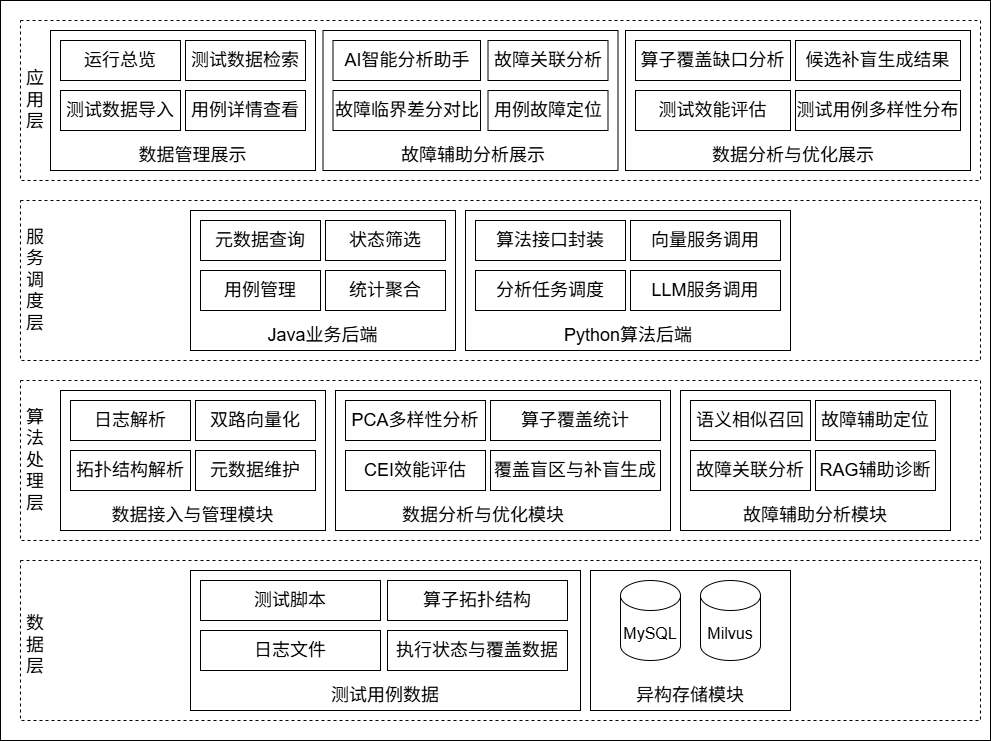
\includegraphics[width=0.85\textwidth]{figure/system_arc.png}
\caption{系统总体架构图}
\label{fig:system_architecture}
\end{figure}

数据层保存系统运行所需的数据资源，
分为测试用例数据和异构存储模块两部分。
测试用例数据由测试脚本、日志文件、算子拓扑结构、执行状态与覆盖数据等组成。
异构存储模块由MySQL和Milvus共同承担，
其中MySQL保存结构化元数据、状态字段和覆盖统计结果，
Milvus保存日志向量和结构向量，
两者共同实现条件查询、相似用例召回，以便后续分析。

算法处理层提供系统分析能力，
按照数据处理方向划分为数据接入与管理模块、数据分析与优化模块和故障辅助分析模块。
数据接入与管理模块负责日志解析、拓扑结构解析、双路向量化和元数据维护；
数据分析与优化模块负责PCA多样性分析、算子覆盖统计、CEI效能评估以及覆盖盲区与补盲生成；
故障辅助分析模块负责语义相似召回、故障辅助定位、故障关联分析和RAG辅助诊断。
这些算法能力根据上层请求被调用，
处理结果再经由服务调度层返回应用层展示。

服务调度层位于应用层和算法处理层之间，
负责接收前端请求、组织查询或分析流程，并把结果整理后返回。
这一层由Java业务后端和Python算法后端共同承担。
Java业务后端负责元数据查询、状态筛选、用例管理和统计聚合等业务请求；
Python算法后端负责算法接口封装、向量服务调用、分析任务调度和LLM服务调用。
具体到实现上，前端按接口类型选择后端：
常规业务查询、语义检索以及RAG问答请求都先走Java业务后端，
其中语义检索和RAG问答随后由Java转发到Python算法后端；
数据导入、覆盖分析、效能评估、多样性分析、故障关联分析以及候选补盲生成这类算法请求则直接调用Python算法后端。
这种划分让结构化业务查询和算法接口调用保持相对清晰的边界。

应用层面向开发者提供Web交互界面，
按照展示内容划分为数据管理展示、故障辅助分析展示和数据分析与优化展示三类。
数据管理展示包括运行总览、用例管理、测试数据检索、测试数据导入和用例详情查看，
主要用于监控系统运行状态、筛选检索和导入模糊测试用例，并管理测试用例数据。
故障辅助分析展示包括AI智能分析助手、故障关联分析、故障临界差分对比和用例故障定位，
主要用于呈现相似历史用例、候选算子节点、参数差分和辅助诊断报告。
数据分析与优化展示包括算子覆盖缺口分析、候选补盲生成结果、测试效能评估和测试用例多样性分布，
主要用于观察测试集覆盖、分布和用例效能。

\section{系统技术栈选型}
\label{sec:tech_stack}

基于系统的分层架构，本系统的技术栈选型围绕前端交互、业务调度、算法处理和数据存储四个方面展开。
相关选择主要由系统中的数据形态、算法依赖和展示需求决定。

前端采用Vue 3框架配合TypeScript开发。
本系统前端包含较多状态联动，
包括测试用例筛选条件、分页结果和详情面板等前端状态。
Vue 3的组合式API适合把这些逻辑拆成相对独立的状态单元。
TypeScript则用来约束接口返回的数据结构，
减少前后端字段变更带来的运行时错误。
UI组件库选用Element Plus，
它的表格、表单和对话框等组件能够覆盖管理系统的需求。
散点图和热力图渲染基于ECharts完成，
以满足管理界面中筛选、悬停和局部查看等交互需求。

业务后端层采用Java 17和Spring Boot 3框架。
这一层面对的是结构化业务数据和前端请求组织，
主要处理常规的业务查询和异常响应。
数据访问层使用Spring Data JPA/Hibernate作为ORM工具，
通过实体类映射\texttt{test\_case\_metadata}表，
常规查询由Repository接口派生方法完成，
统计类的结果则使用Repository中的原生SQL聚合查询。
这一层同时作为部分算法能力的代理入口，
主要转发语义检索和RAG问答请求。

算法后端层采用Python 3.11和FastAPI框架。
这一层主要依赖语义编码、向量检索和数据处理相关的组件，
支撑向量化、检索和数据处理等算法任务。
FastAPI用来把这些算法能力封装成RESTful接口，
既供Java业务后端代理调用，
也供前端分析页面直接调用。

存储层采用MySQL 8.0和Milvus 2.3.4共同管理系统数据。
本系统的数据包含两种主要形态：
一类是\texttt{case\_uid}、执行状态、覆盖贡献数据和CEI得分等结构化字段；
另一类是由语义编码模型生成的日志向量和结构向量。
结构化字段需要支持条件筛选、分页、排序等，
因此由MySQL保存。
高维语义向量需要支持相似度检索，
因此由Milvus建立向量索引并完成相似向量召回。
每条测试用例入库时，
算法后端先把日志向量和结构向量写入Milvus并获得向量主键，
再把\texttt{case\_uid}、执行状态、覆盖数据和向量主键写入MySQL。
查询时，结构化筛选以MySQL为主；
语义检索先由Milvus返回相似向量主键，
再根据MySQL中保存的关联字段查找完整元数据。
这种异构双库存储方式让MySQL负责元数据记录和跨库关联，
Milvus负责向量相似度召回，
共同为检索、分析和展示功能提供数据支撑。

\section{本章小结}

本章在分析深度学习框架模糊测试产物管理与分析需求的基础上，完成了系统的总体设计。首先，明确了系统在功能、输入输出以及补充说明等维度的具体需求；其次，设计了包含数据层、算法处理层、服务调度层和应用层的四层系统总体架构，理清了各层组件及其逻辑调用关系；最后，进行了系统技术栈选型，确定前端采用Vue 3与TypeScript，业务后端采用Java Spring Boot与Hibernate，算法后端采用Python FastAPI，数据存储采用MySQL与Milvus。本章总体设计为后续系统模块的具体实现与算法应用提供了清晰的框架指导。


% !Mode:: "TeX:UTF-8"
\chapter{系统详细设计与主要算法}

本章依据第三章给出的系统总体架构图展开详细设计，
重点描述算法处理层中的核心模块，
以及这些模块与数据层之间的必要关联，
包括数据接入与特征表示、异构存储、故障辅助分析以及数据分析与优化等内容。

\section{数据接入与特征表示设计}

数据接入与特征表示设计对应架构图中的数据接入与管理模块。
该部分负责把Fuzzing产物中的日志、测试脚本和算子拓扑结构整理为可检索、可分析的信息。
其中，日志解析用于提取错误类型和运行状态，
双路向量化用于把日志语义和模型结构分别映射到向量空间。

\subsection{基于分层正则匹配的日志解析模块}

Fuzzing工具输出的崩溃日志在格式上不统一。
同一条记录中可能同时包含多层运行时信息以及多线程交织产生的乱序输出。
日志解析模块接收原始崩溃日志及相关测试信息，
将其中稳定的字段提取为后续分析所需的元数据。

本系统设计的LogParser模块采用分层正则匹配策略，
将解析过程分解为错误分类与字段提取两个独立阶段。
在错误分类阶段，模块维护一张带有优先级顺序的错误模式表，
涵盖八种PyTorch测试中常见的错误类别，如表\ref{tab:error_categories}所示。

\begin{table}[htbp]
\centering
\caption{LogParser模块支持的八种标准化错误类别}
\label{tab:error_categories}
\begin{tabular}{lll}
\toprule
类别标识 & 中文描述 & 典型触发关键词 \\
\midrule
\texttt{cuda\_oom} & CUDA显存溢出 & cuda out of memory, oom \\
\texttt{shape\_mismatch} & 张量维度不匹配 & size mismatch, incompatible \\
\texttt{segfault} & 内存段错误 & segmentation fault, signal 11 \\
\texttt{timeout} & 执行超时 & timeout, exceeded maximum \\
\texttt{device\_mismatch} & 设备不匹配 & expected.*device \\
\texttt{index\_error} & 索引越界 & index out of, out of bounds \\
\texttt{type\_error} & 类型错误 & type error, invalid type \\
\texttt{nan\_inf} & 数值异常 & nan, inf, not a number \\
\bottomrule
\end{tabular}
\end{table}

模块将输入文本统一转换为小写后，依照表中自上而下的优先级顺序扫描关键词。
一旦命中即终止扫描并返回对应错误类别。
优先级排列主要依据异常处理时的排查优先级：
显存溢出与段错误属于系统级致命异常，排在最前；
数值异常属于静默型偏差，排在最后。
对于不命中任何模式的日志，模块将其归入\texttt{other}类别。
该分类结果用于为后续故障辅助定位和检索分析提供错误标签。

字段提取阶段则针对不同数据类型分别准备了一组正则表达式，
从原始日志中抽取出以下六项结构化字段：

（1）错误类型（error\_type）。
面向Python异常，模块使用形如\texttt{(\textbackslash w+Error):}的正则匹配得到类名；
遇到C++层的段错误，则改为检测是否出现\texttt{Segmentation Fault}关键字。

（2）张量维度（tensor\_shapes）。
PyTorch的维度报错主要包含方阵表示法\texttt{m1: [32 x 512]}，
部分报错还会直接给出匿名形状\texttt{[32 x 512]}。
模块为这两类格式分别编写正则表达式并按优先级依次尝试，
成功匹配后输出为\texttt{\{name, shape\}}结构化字典列表。

（3）框架源码位置（source\_location）。
C++侧报错一般带有类似\texttt{at /pytorch/.../}\allowbreak\texttt{THTensorMath.cpp:41}的源码路径，
Python侧则使用\texttt{File "xxx.py", line 42}这样的格式。
模块分别准备了正则表达式，用于取出文件名、行号和模块路径。

（4）显存信息（memory\_info）。
仅在\texttt{cuda\_oom}类别下激活。
模块提取三组数值：请求分配量、已分配量与设备总容量。

（5）设备信息（device\_info）。
通过全局扫描\texttt{cuda:N}与\texttt{cpu}标识符提取，去重后输出为列表。

（6）原始消息（raw\_message）。
保留未经处理的完整日志文本，供RAG模块作为LLM上下文素材。

\subsection{双路向量化特征表示方法}

如第二章所述，本系统采用Sentence-BERT编码模型将离散文本映射为384维稠密浮点向量。
针对Fuzzing产物的异构特性，系统设计了两条并行的向量化路径。

第一条路径为报错堆栈语义表征。
模块把用例的\texttt{error\_message}字段直接送入Sentence-BERT编码器。
遇到成功执行、没有错误信息的用例，则补充占位文本
\texttt{"Success: [status] - Model executed OK"}进行编码。
这条路径产出的向量写入Milvus中的\texttt{fuzzing\_logs}集合，
供后续语义检索使用。

第二条路径为图拓扑序列投影。
模块将测试用例的模型结构字典序列化为标准化文本，
格式为\texttt{"Model structure: layers=[...],}\allowbreak\texttt{ connections=...,}\allowbreak\texttt{ depth=N,}\allowbreak\texttt{ operators=[...]"}。
该文本经Sentence-BERT编码后产出的向量存入Milvus的\texttt{fuzzing\_structure}集合，
用于多样性分析与拓扑相似性召回。

为了避免重复加载开销，两条路径共用同一个all-MiniLM-L6-v2模型实例。
每个测试用例经过该处理后会得到两个独立的384维向量。

\section{异构存储模块设计}

异构存储模块用于连接数据接入的结果与后续分析算法。
结合第三章的技术栈选型，
系统采用MySQL与Milvus组合保存测试用例数据。

在数据组织上，MySQL中的\texttt{test\_case\_metadata}表以\texttt{case\_uid}作为业务标识，
保存用例状态、错误信息、分支边覆盖数、执行耗时和扩展参数等信息。
Milvus维护\texttt{fuzzing\_logs}和\texttt{fuzzing\_structure}两个集合，
分别对应报错堆栈语义向量和模型结构向量。
两类数据不放在同一数据库中，
主要是因为结构化筛选和相似度检索对存储模型的要求不同。

跨库关联通过MySQL中保存的向量主键完成。
数据接入阶段，系统先完成日志文本和结构文本的向量化，
再将两路向量写入Milvus并取得各自的主键标识
（\texttt{structure\_vector\_id}与\texttt{log\_vector\_id}）。
结构向量主键写入MySQL的\texttt{vector\_id}字段，
结构向量主键与日志向量主键同时写入\texttt{parameters}字段，
并与结构化元数据和\texttt{case\_uid}一同保存。
后续检索时，系统可先在Milvus中召回相似向量，
再依据返回的主键查询MySQL中的元数据。
这种设计避免在Milvus中保存业务字段，
也便于在MySQL中维护用例状态、覆盖数据和清退标记。

\section{故障辅助分析模块设计}

故障辅助分析模块对应系统架构图中的故障辅助分析能力，
主要包括单用例故障辅助定位、语义相似召回、故障关联分析和RAG辅助诊断。
其中，故障辅助定位用于在用例详情中标注候选算子节点；
语义相似召回和RAG辅助诊断用于组织历史案例并生成辅助诊断报告；
故障关联分析则结合相似成功样本与崩溃样本，
提取候选边界条件和参数差分。

\subsection{基于DFS拓扑回溯的故障辅助定位模块}

日志解析完成后，系统需要将结构化错误信息与测试用例的计算图结构相结合，
定位出可能与崩溃相关的候选算子节点位置。
本系统设计的FaultLocator模块通过逆向邻接表与DFS回溯实现该功能，
帮助用户缩小排查范围。

逆向邻接表的构建过程如下。
系统将测试用例中的算子拓扑统一表示为有向图$G=(V,\mathcal{E})$，
其中节点集合$V$表示算子节点，边集合$\mathcal{E}$表示数据的流向。
设正向边$(o_i,o_j)\in\mathcal{E}$表示数据由$o_i$流向$o_j$，
则逆向邻接表中记录$o_j$到$o_i$的反向关系。

具体定位过程如算法\ref{alg:dfs_fault_locator}所示。

\begin{algorithm}[htbp]
\caption{基于DFS回溯的候选算子定位算法}
\label{alg:dfs_fault_locator}
\begin{algorithmic}[1]
\REQUIRE 结构化错误信息$E$，算子有向图$G=(V,\mathcal{E})$
\ENSURE 候选算子节点列表$\mathcal{L}$
\STATE 根据边集合$\mathcal{E}$构建逆向邻接表$\mathbf{A}^{-1}$
\STATE 根据$E$中的错误类别选择错误相关算子集合$\mathcal{M}$
\STATE 根据$E$确定候选触发节点集合$\mathcal{T}$；若无法确定，则令$\mathcal{T}\leftarrow V$
\STATE $\mathcal{L} \leftarrow \emptyset$
\FOR{each trigger node $t \in \mathcal{T}$}
    \STATE 从$t$开始沿$\mathbf{A}^{-1}$执行DFS回溯
    \FOR{each visited node $o_i$}
        \IF{$o_i \in \mathcal{M}$ or $o_i$ matches a risky topology pattern}
            \STATE 计算候选置信度$score(o_i)$并生成推理理由
            \STATE $\mathcal{L} \leftarrow \mathcal{L} \cup \{(o_i, \mathrm{id}(o_i), score(o_i), reason)\}$
        \ENDIF
        \IF{$o_i \in \mathcal{M}$ or depth exceeds threshold or $\mathbf{A}^{-1}(o_i)=\emptyset$}
            \STATE 停止当前回溯分支
        \ENDIF
    \ENDFOR
\ENDFOR
\STATE 对$\mathcal{L}$按置信度降序排序
\RETURN $\mathcal{L}$
\end{algorithmic}
\end{algorithm}

其中，错误相关算子集合$\mathcal{M}$根据错误类型确定。
例如，维度变换错误主要关注Linear、Conv2d和Reshape等算子；
高显存问题优先检查Conv类和Attention类算子。
这里的置信度只用于排序候选节点，不表示真实缺陷概率。
该列表将传递给前端在计算图可视化中高亮标注候选节点。

\subsection{语义相似召回与RAG辅助诊断}

当用户针对某一崩溃用例发起诊断请求时，
系统先从历史用例中召回语义相近的记录，
再把召回结果作为RAG上下文交给LLM生成辅助诊断报告。
其处理过程如算法\ref{alg:rag_retrieval}所示。

\begin{algorithm}[htbp]
\caption{语义相似召回与RAG辅助诊断算法}
\label{alg:rag_retrieval}
\begin{algorithmic}[1]
\REQUIRE 用户查询$q$，最终返回数量$K$
\ENSURE 召回用例集合$\mathcal{C}$，辅助诊断报告$R$
\STATE $v_q \leftarrow \text{SentenceBERT}(q)$
\STATE 在\texttt{fuzzing\_structure}中检索与$v_q$最相似的前$3K$个结构候选
\STATE 在\texttt{fuzzing\_logs}中检索与$v_q$最相似的前$3K$个日志候选
\STATE 根据$q$中的结构关键词和日志关键词比例计算两路融合权重
\STATE 合并两路候选结果，并按融合得分截取前$K$个用例，记为$\mathcal{C}$
\STATE 根据$\mathcal{C}$中的主键从MySQL反查完整元数据
\STATE 将元数据和用户查询$q$组装为RAG上下文提示词$P$
\STATE $R \leftarrow \text{LLM}(P)$
\RETURN $\mathcal{C}, R$
\end{algorithmic}
\end{algorithm}

LLM基于检索到的真实历史案例生成辅助诊断报告，
为开发者提供故障排查参考信息。

\subsection{故障关联分析}

故障关联分析中的候选边界条件分析模块借鉴经典的Daikon动态不变量推断范式\cite{ref_daikon}，
在成功样本与崩溃样本构成的对照组中扫描候选约束，
输出候选边界条件，用于辅助分析崩溃触发条件。

候选边界条件分析的输入为一个目标崩溃用例。
模块先提取该用例的图拓扑结构向量，
在Milvus的\texttt{fuzzing\_structure}集合中执行余弦相似度检索，
分别召回拓扑结构相似但执行成功的10个用例（健康组$\mathcal{S}$）
与执行失败的10个用例（崩溃组$\mathcal{F}$）。
召回条件为结构相似度大于0.85，确保对照样本与目标用例的算子组合足够相近。

召回完成后，模块对每个用例的嵌套参数字典执行展平操作。
DL测试用例的参数空间通常包含模型结构字典、层配置子字典、标量参数和列表参数。
展平操作把这些嵌套结构转成一维键值对，
同时过滤向量主键、覆盖率等无关字段。
过滤后的键值对集合仅保留与算子配置直接相关的参数。

展平完成后，模块计算健康组与崩溃组所有样本的键集合交集，
其中$\Phi(\cdot)$表示参数展平后的键值对集合：
\begin{equation}
\label{eq:common_keys}
\mathcal{K} = \bigcap_{s \in \mathcal{S}} \text{keys}(\Phi(s)) \;\cap\; \bigcap_{f \in \mathcal{F}} \text{keys}(\Phi(f))
\end{equation}
仅在$\mathcal{K}$中的键才进入后续的候选约束扫描环节。

模块在公共键集合$\mathcal{K}$上扫描三层模板池，
包括单变量阈值与奇偶性模板、双变量约束与整除关系模板，
以及三变量约束模板。
仅当某条候选约束同时满足“成功全票通过”与“失败全票否决”的双重验证时，
该约束才被加入候选边界条件集合。

上述三层扫描的双重验证判据以算法\ref{alg:dual_verify}的伪代码形式给出。

\begin{algorithm}[htbp]
\caption{双重验证判据——候选边界条件提取算法}
\label{alg:dual_verify}
\begin{algorithmic}[1]
\REQUIRE 健康组展平参数集合 $\mathcal{S}_{\text{flat}} = \{s_1, s_2, \ldots, s_{|\mathcal{S}|}\}$
\REQUIRE 崩溃组展平参数集合 $\mathcal{F}_{\text{flat}} = \{f_1, f_2, \ldots, f_{|\mathcal{F}|}\}$
\REQUIRE 公共键集合 $\mathcal{K} = \{k_1, k_2, \ldots, k_n\}$
\ENSURE 候选约束集合 $\mathcal{R} = \{\}$
\FOR{each candidate predicate $\phi(k_{i_1}, \ldots, k_{i_p})$ in template pool}
    \STATE $\textit{success\_pass} \leftarrow \text{True}$
    \STATE $\textit{failure\_reject} \leftarrow \text{True}$
    \FOR{each $s \in \mathcal{S}_{\text{flat}}$}
        \IF{$\phi(s[k_{i_1}], \ldots, s[k_{i_p}])$ is False}
            \STATE $\textit{success\_pass} \leftarrow \text{False}$
            \STATE \textbf{break}
        \ENDIF
    \ENDFOR
    \IF{$\textit{success\_pass}$ is True}
        \FOR{each $f \in \mathcal{F}_{\text{flat}}$}
            \IF{$\phi(f[k_{i_1}], \ldots, f[k_{i_p}])$ is True}
                \STATE $\textit{failure\_reject} \leftarrow \text{False}$
                \STATE \textbf{break}
            \ENDIF
        \ENDFOR
    \ENDIF
    \IF{$\textit{success\_pass}$ is True \AND $\textit{failure\_reject}$ is True}
        \STATE $\mathcal{R} \leftarrow \mathcal{R} \cup \{\phi\}$
    \ENDIF
\ENDFOR
\RETURN $\mathcal{R}$
\end{algorithmic}
\end{algorithm}

提取出的约束集合$\mathcal{R}$经去重后按优先级排序：
多变量约束排在单变量约束之前，
因为多变量约束包含更丰富的变量间交互信息。
排序后的约束列表即为该崩溃用例的候选边界条件集合，
用于为开发者提供后续排查线索。

最后，系统把候选约束集合$\mathcal{R}$、参数差分和相关测试上下文组装为提示词，
由LLM生成用于解释候选约束的辅助诊断报告。
前端将候选数学公式和辅助诊断报告并列展示。

\section{数据分析与优化模块设计}

数据分析与优化模块对应架构图中的数据分析与优化能力。
该模块针对测试集整体质量，
提供多样性分布观察、效能评估、算子覆盖缺口分析以及候选补盲测试脚本生成等功能。

\subsection{基于PCA的测试集多样性分析}

Fuzzing过程会不断产生测试用例。
这些用例在语义向量空间中的分布，
可以用于观察测试集在算子组合和参数结构上的差异。
由于384维向量空间不便直接查看，
系统需要先将它压缩到二维平面。

本系统在批量更新后或用户请求多样性分析时，对当前样本集合统一执行PCA降维。
具体流程为：取当前参与分析的测试用例结构向量矩阵$\mathbf{X} \in \mathbb{R}^{b \times 384}$
（$b$为参与降维的样本数量），计算协方差矩阵并提取前两个主成分方向，
将每个样本投影至二维坐标$(x_i, y_i)$。
投影后的坐标经最小-最大归一化映射至$[-1, 1]$区间，
存入MySQL的\texttt{parameters}字段中的\texttt{vis\_x}与\texttt{vis\_y}键。

前端散点图基于上述二维坐标渲染。
用户可观察测试集的空间分布形态：
若散点呈现明显的簇状聚集，说明当前Fuzzing策略可能集中在有限的算子组合区域内；
若散点分布较为分散，说明测试输入在模型结构或参数组合上具有更高差异。
稀疏区域对应尚未被充分测试的算子拓扑组合，
可作为后续补盲策略的参考方向。

\subsection{CEI覆盖效能指数量化模型}

CEI用来描述单个测试用例在覆盖贡献数据和计算成本之间的关系，其数学定义如下：
\begin{equation}
\label{eq:cei}
\mathrm{CEI} = \frac{E_{\text{edge}}}{\displaystyle\sum_{i=1}^{m} w_i \cdot c_i}
\end{equation}
其中$E_{\text{edge}}$为该用例的分支边覆盖数，
$m$为该用例计算图中不同算子类型的数量，
$c_i$为第$i$类算子在计算图中的出现次数，
$w_i$为第$i$类算子对应的权重系数。
公式分母表示按算子类型和出现次数估计的计算成本，
不包含执行耗时变量；执行耗时可以作为实验评估指标单独记录。

算子权重$w_i$的设计原则是：
计算量越大、参数空间越大的算子，赋予的权重越大，
因为这类算子消耗的执行资源更多，却不一定带来更高的覆盖贡献。
表\ref{tab:operator_weight}列出本系统的部分算子权重。

\begin{table}[htbp]
\centering
\caption{部分算子的CEI权重基准}
\label{tab:operator_weight}
\begin{tabular}{llr}
\toprule
算子类别 & 典型算子 & 权重$w_i$ \\
\midrule
计算密集型 & Conv2d, Conv3d, Linear, LSTM & 3.0 \\
注意力机制 & MultiHeadAttention, Transformer & 4.0 \\
归一化层 & BatchNorm2d, LayerNorm, GroupNorm & 1.5 \\
池化层 & MaxPool2d, AvgPool2d, AdaptiveAvgPool & 1.0 \\
激活函数 & ReLU, Sigmoid, Tanh, GELU & 0.5 \\
结构操作 & Flatten, Reshape, Dropout, Concat & 0.3 \\
\bottomrule
\end{tabular}
\end{table}

系统在执行清退时，把全库CEI中位数的$\alpha$倍作为淘汰阈值。
CEI低于这个阈值的用例在当前指标下覆盖收益相对较低，会进入级联删除流程。
这一流程主要帮助识别冗余数据，
减少它们对存储空间和后续分析结果的干扰。

当用户确认执行清退操作时，
系统需要按照MySQL中保存的向量主键同步处理Milvus向量记录。
具体流程分为三步。
第一步，从MySQL中批量查询满足清退条件的记录，
提取其\texttt{vector\_id}、
\texttt{parameters.structure\_}\allowbreak\texttt{vector\_id}
和\texttt{parameters.log\_vector\_id}。
第二步，调用Milvus的\texttt{delete}接口按主键删除两个集合中的对应向量。
第三步，在MySQL中执行\texttt{DELETE}语句移除对应元数据记录。

\subsection{算子覆盖缺口分析}

除了对单个用例做效能评估之外，系统还需要从全局视角分析测试盲区，
即在当前已出现算子和常用算子范围内，
尚未被测试集覆盖的算子组合模式。

系统不直接枚举PyTorch中的全部公开算子，
而是构造用于缺口分析的候选算子集合$\mathcal{O}$。
该集合由两部分组成：
一部分是当前测试集中已经出现过的算子类型，
另一部分是预设的20个常用PyTorch算子类型。
记当前测试集已出现算子集合为$\mathcal{O}_{\text{seen}}$，
常用算子集合为$\mathcal{O}_{\text{common}}$，
则有：
\begin{equation}
\label{eq:operator_pool}
\mathcal{O} = \mathcal{O}_{\text{seen}} \cup \mathcal{O}_{\text{common}}
\end{equation}

全局邻接矩阵$\mathbf{A} \in \{0,1\}^{|\mathcal{O}| \times |\mathcal{O}|}$
记录了当前测试集中已经出现过的算子对组合关系。

盲区提取通过集合差运算来完成。
定义候选可行算子对全集$\mathcal{E}_{\text{all}}$为$\mathcal{O}$中
所有在PyTorch算子语义下合法的算子组合（排除不合理的组合，
例如\texttt{Softmax}不能直接接\texttt{Conv2d}的通道输入端）。
已覆盖算子对集合$\mathcal{E}_{\text{covered}} = \{(i,j) \mid \mathbf{A}[i][j] = 1\}$。
盲区集合定义为：
\begin{equation}
\label{eq:blind_spots}
\mathcal{B} = \mathcal{E}_{\text{all}} \setminus \mathcal{E}_{\text{covered}}
\end{equation}

盲区集合$\mathcal{B}$中的每个元素$(o_i, o_j)$表示一对还没被测试的算子衔接。
系统把$\mathcal{B}$按算子类别分组后输出为结构化列表。
这一列表会作为后续补盲模块的输入目标。

\subsection{覆盖缺口驱动的候选补盲测试脚本生成}

盲区集合$\mathcal{B}$标记了当前测试集的覆盖缺口。
本系统通过构造结构化提示词，
让LLM生成候选补盲测试脚本来覆盖这些缺口。

结构化提示词的设计如表\ref{tab:prompt_template}所示：

\begin{table}[htbp]
\centering
\caption{RAG补盲提示词模板结构}
\label{tab:prompt_template}
\begin{tabular}{lp{10cm}}
\toprule
板块 & 内容设计 \\
\midrule
\textbf{System} &
“你是一个深度学习模糊测试专家助手。\allowbreak{}
你的任务是根据用户问题和检索到的测试用例上下文，\allowbreak{}
提供专业的分析和建议。请基于提供的测试用例数据给出具体建议；\allowbreak{}
如果问题涉及错误分析，给出可疑条件和排查方向；\allowbreak{}
如果问题涉及优化建议，给出可行的改进方案。\allowbreak{}
保持回答简洁专业，使用中文回答。” \\
\midrule
\textbf{Context} &
注入从Milvus召回的$K$个最相似历史用例的结构化摘要，
每条包含：用例编号、执行状态和错误信息摘要等。
格式为“用例N: [case\_uid] - 状态: [status] -
算子: [operators]”。\\
\midrule
\textbf{Target} &
明确列出当前需要补盲的算子对列表，
例如“请生成一个包含\allowbreak{}\texttt{Conv2d->}\allowbreak\texttt{GroupNorm->LSTM}\allowbreak{}连接链的PyTorch模型脚本”。
包含目标算子的参数范围约束
（如\texttt{in\_channels}$\in [1, 512]$、\allowbreak{}%
\texttt{kernel\_size}$\in [1, 7]$）。\\
\midrule
\textbf{Constraint} &
语法限制与输出格式要求：
“输出应为可检查的候选Python脚本；
模型应继承\texttt{torch.nn.Module}；\allowbreak{}
\texttt{forward}方法应接受形状为\allowbreak{}%
\texttt{[batch, channels, H, W]}的输入张量；
脚本末尾应包含推理调用语句。”\\
\bottomrule
\end{tabular}
\end{table}

上述四板块模板在工程实现中的作用如下：
System板块限定LLM的角色边界，减少它偏离测试生成任务；
Context板块注入真实的历史数据作为参考，减少无上下文生成的问题；
Target板块指定覆盖目标，减少LLM生成已有冗余用例的可能；
Constraint板块给出语法和结构约束，让输出更便于后续检查和执行验证。

LLM生成的候选补盲测试脚本经过必要的检查和确认后，
可以作为后续测试输入的候选材料，
再由开发者确认是否进入数据接入流程，
形成“发现盲区→生成候选补盲测试脚本→执行验证→后续分析”的处理流程。
% !Mode:: "TeX:UTF-8"
\chapter{系统实现与功能展示}

\section{开发环境与工具配置}

本系统的开发、测试和部署涉及前端、业务后端、算法后端和底层物理执行四个层面。
为了让系统实现和后续实验环境保持一致，
本章和第六章采用同一套软硬件配置。
表\ref{tab:dev_env}列出系统实现和实验验证所使用的主要环境配置。

\begin{table}[htbp]
\centering
\caption{开发环境与工具配置清单}
\label{tab:dev_env}
\small
\begin{tabular}{>{\raggedright\arraybackslash}p{2.1cm}>{\raggedright\arraybackslash}p{3.9cm}>{\raggedright\arraybackslash}p{2.7cm}>{\raggedright\arraybackslash}p{3.8cm}}
\toprule
类别 & 名称 & 版本/规格 & 用途 \\
\midrule
操作系统 & Windows 11 + WSL2 (Ubuntu 22.04) & 23H2 & 开发与物理执行 \\
处理器 & Intel Core i7-12700H & 14核20线程 & 编译与实验运行 \\
内存 & DDR4 & 16\,GB & 数据导入与服务运行 \\
显卡 & NVIDIA RTX 3060 Laptop GPU & 6\,GB GDDR6 & CUDA算子执行 \\
CUDA工具链 & CUDA Toolkit & 11.8 & GPU运行时环境 \\
前端框架 & Vue 3 + TypeScript & 3.3 / 5.3 & 单页应用开发 \\
UI组件库 & Element Plus & 2.4 & 界面组件渲染 \\
构建工具 & Vite & 5.0 & 前端热更新打包 \\
业务后端 & Java Spring Boot + JPA/Hibernate & 3.2 / 8080端口 & 结构化数据管理与代理转发 \\
JDK & OpenJDK & 17 & Java运行时 \\
算法后端 & Python FastAPI & 0.104 / 5000端口 & 算法服务与RAG \\
Python & CPython & 3.11 & 算法后端运行时 \\
关系数据库 & MySQL & 8.0 & 结构化元数据存储 \\
向量数据库 & Milvus & 2.3.x & 高维语义向量存储 \\
语义编码 & all-MiniLM-L6-v2 & 384维输出 & 日志与脚本结构向量化 \\
深度学习框架 & PyTorch & 2.1.0源码编译 & 物理执行与覆盖率采集 \\
覆盖率工具 & Gcov / LCOV & GCC 11 / 1.16 & C++层探针采集 \\
前端图表 & ECharts & --- & 散点图、热力图与统计图表展示 \\
\bottomrule
\end{tabular}
\end{table}

当前实现中，
前端运行在Vite开发服务器上（默认端口5173），
通过Axios访问Java Spring Boot后端和Python FastAPI后端。
Java后端（端口8080）主要负责结构化数据管理与部分代理转发，
Python后端（端口5000）主要负责语义检索、候选边界条件分析、
CEI分析和候选补盲建议等算法处理。

底层物理执行环境部署在WSL2中的Ubuntu 22.04子系统里。
这个子系统里安装了带Gcov探针的PyTorch编译版本，
以及独立的Python虚拟环境\texttt{venv\_pytorch}。
物理执行层通过\texttt{multiprocessing}模块的\texttt{spawn}启动方式创建独立的子进程，
在WSL环境下调用插桩后的PyTorch库执行测试脚本，
采集覆盖贡献数据。

\section{后端主要模块实现}

\subsection{Python FastAPI算法后端实现}

Python FastAPI算法后端主要负责语义编码、向量检索、PCA降维、Daikon候选边界条件分析和RAG相关接口。
服务初始化阶段建立Milvus连接、
加载两个向量集合及Sentence-BERT编码模型；
MySQL连接则在处理具体请求时按需建立。

该后端注册了数据导入、语义检索、统计分析、候选边界条件分析、CEI清退和补盲建议等API路由。
表\ref{tab:api_routes}列出主要路由的方法、路径和功能摘要。

\begin{table}[htbp]
\centering
\setlength{\tabcolsep}{6pt}
\renewcommand{\arraystretch}{1.4}
\caption{Python FastAPI算法后端API路由清单}
\label{tab:api_routes}
\begin{tabular}{llp{7.1cm}}
\toprule
方法 & 路径 & 功能摘要 \\
\midrule
POST & \texttt{/api/ingest} & 批量导入测试用例，执行双路向量化与写入 \\
POST & \texttt{/api/search} & 语义检索并返回匹配用例 \\
POST & \texttt{/api/ask} & RAG辅助诊断问答 \\
GET & \texttt{/api/recent\_cases} & 获取最近入库的测试用例列表 \\
GET & \texttt{/api/statistics} & 全局统计概览 \\
GET & \texttt{/api/analysis/}\allowbreak\texttt{coverage-gaps} & 算子覆盖热力图与覆盖缺口统计 \\
GET & \texttt{/api/analysis/}\allowbreak\texttt{efficiency} & CEI效能统计与散点分布 \\
GET & \texttt{/api/analysis/}\allowbreak\texttt{error-patterns} & 错误模式交叉聚类分析 \\
GET & \texttt{/api/analysis/}\allowbreak\texttt{correlations} & 算子-错误关联矩阵 \\
POST & \texttt{/api/analysis/}\allowbreak\texttt{fault-boundary} & 候选边界条件分析与辅助诊断报告生成 \\
POST & \texttt{/api/suggest} & 基于历史数据的变异建议生成 \\
POST & \texttt{/api/auto-generate}\allowbreak\texttt{-from-gaps} & 覆盖盲区候选补盲测试脚本生成 \\
POST & \texttt{/api/analysis/}\allowbreak\texttt{efficiency/prune} & CEI阈值清退预览与执行 \\
\bottomrule
\end{tabular}
\end{table}

语义检索接口\texttt{/api/search}的请求体以\texttt{query}字段为核心，
用于接收自然语言查询文本。
请求模型还包含\texttt{top\_k}、\texttt{search\_mode}、
\texttt{structure\_weight}和\texttt{log\_weight}等字段，
用于描述检索模式和结构向量与日志向量的融合权重；
响应体包含\texttt{total}、\texttt{results}、\texttt{query}、
\texttt{search\_mode}和\texttt{query\_intent}等字段，
其中\texttt{results}数组保存匹配用例及其相似度得分。

候选边界条件分析接口\texttt{/api/analysis/fault-boundary}的请求体包含
\texttt{failed\_case\_uid}字段，
用于指定待分析的崩溃用例。
响应体包含\texttt{failed\_case}、\texttt{successful\_case}、
\texttt{diff}、\texttt{batch\_context}、\texttt{daikon\_violations}、
\texttt{daikon\_validation}和\texttt{boundary\_rule}等字段。
其中，\texttt{diff}用于展示参数差异，
\texttt{daikon\_validation}保存待人工验证的正反样例，
\texttt{boundary\_rule}保存辅助诊断报告。

\subsection{Java Spring Boot业务后端实现}

Java Spring Boot后端承担基础业务数据管理和前端请求组织功能，
监听8080端口，并通过Spring Data JPA与MySQL交互。
该后端提供的主要API路由如表\ref{tab:java_api_routes}所示。

\begin{table}[htbp]
\centering
\setlength{\tabcolsep}{6pt}
\renewcommand{\arraystretch}{1.25}
\caption{Java Spring Boot业务后端API路由清单}
\label{tab:java_api_routes}
\begin{tabular}{llp{7.1cm}}
\toprule
方法 & 路径 & 功能摘要 \\
\midrule
GET & \texttt{/api/cases} & 分页查询测试用例，可按状态过滤 \\
GET & \texttt{/api/cases/recent} & 获取最近测试用例，用于运行总览展示 \\
GET & \texttt{/api/cases/\{id\}} & 按物理主键查询单个测试用例 \\
GET & \texttt{/api/cases/uid/}\allowbreak\texttt{\{caseUid\}} & 按业务标识符查询单个测试用例 \\
GET & \texttt{/api/statistics/}\allowbreak\texttt{overview} & 返回总数、崩溃数、平均耗时和平均覆盖数据 \\
GET & \texttt{/api/statistics/}\allowbreak\texttt{status} & 返回不同状态的用例数量 \\
GET & \texttt{/api/statistics/}\allowbreak\texttt{errors} & 返回错误类型排行 \\
POST & \texttt{/api/search} & 代理语义检索请求到Python服务 \\
POST & \texttt{/api/ask} & 代理RAG辅助诊断请求到Python服务 \\
\bottomrule
\end{tabular}
\end{table}

其中，统计接口组包含三条路由：
\texttt{/api/statistics/overview}返回用例总数、崩溃率和平均执行耗时；
\texttt{/api/statistics/status}返回各状态类别的用例数；
\texttt{/api/statistics/errors}返回错误类型。
这些结果会被封装为前端图表组件可以直接使用的JSON格式。

对语义检索和RAG辅助诊断请求，
Java后端通过Spring Cloud OpenFeign转发到配置项
\texttt{python-service.url}对应的Python服务，
再把响应体返回给前端。

\subsection{数据库表结构与向量集合详细设计}

表\texttt{test\_case\_metadata}
负责存储测试用例结构化元数据。
表\ref{tab:mysql_schema}列出了该表的完整字段设计。

\begin{table}[htbp]
\centering
\caption{MySQL主要表test\_case\_metadata字段设计}
\label{tab:mysql_schema}
\begin{tabular}{llcp{5.5cm}}
\toprule
字段名 & 数据类型 & 主键 & 说明 \\
\midrule
\texttt{id} & BIGINT & 是 & 自增物理主键 \\
\texttt{case\_uid} & VARCHAR(64) & 唯一 & 全局唯一业务标识符 \\
\texttt{status} & VARCHAR(20) & --- & 执行状态（Success/Crash/\allowbreak{}Timeout） \\
\texttt{edge\_coverage} & INT & --- & Gcov采集的分支边覆盖数 \\
\texttt{execution\_time} & FLOAT & --- & 执行耗时（秒） \\
\texttt{error\_message} & TEXT & --- & 原始崩溃日志文本 \\
\texttt{vector\_id} & BIGINT & --- & Milvus结构向量集合中的主键 \\
\texttt{parameters} & JSON & --- & 扩展信息（模型结构、双向量ID、\allowbreak{}PCA坐标等） \\
\texttt{created\_at} & DATETIME & --- & 记录创建时间戳 \\
\texttt{updated\_at} & DATETIME & --- & 记录最后更新时间戳 \\
\bottomrule
\end{tabular}
\end{table}

在\texttt{case\_uid}字段上建立唯一索引，
通过\texttt{ON DUPLICATE KEY UPDATE}语义在重复导入时更新已有记录。
\texttt{parameters}字段采用JSON类型，
保存模型结构字典、PCA降维坐标和Milvus双向量主键等扩展信息。
其中Milvus双向量主键包括\texttt{structure\_vector\_id}和\texttt{log\_vector\_id}。

Milvus侧维护两个独立的向量集合，Schema配置相同。
表\ref{tab:milvus_schema}列出了集合的字段与索引参数。

\begin{table}[htbp]
\centering
\caption{Milvus向量集合Schema与索引配置}
\label{tab:milvus_schema}
\begin{tabular}{lll}
\toprule
配置项 & 参数 & 值 \\
\midrule
集合名称（结构向量） & --- & \texttt{fuzzing\_structure} \\
集合名称（日志向量） & --- & \texttt{fuzzing\_logs} \\
主键字段 & \texttt{id} & INT64，自动生成 \\
向量字段 & \texttt{embedding} & FLOAT\_VECTOR，维度384 \\
索引类型 & \texttt{index\_type} & IVF\_FLAT \\
相似度度量 & \texttt{metric\_type} & COSINE \\
倒排列表数量 & \texttt{nlist} & 128 \\
检索探测簇数 & \texttt{nprobe} & 16 \\
\bottomrule
\end{tabular}
\end{table}

两个集合在服务启动时执行\texttt{collection.load()}操作，
把索引结构和向量数据加载到Milvus的查询节点内存中，
从而降低检索请求触发额外加载的开销。

跨库数据关联通过写入顺序和主键回填共同维护：
结构向量主键写入\texttt{vector\_id}字段，
\texttt{structure\_vector\_id}和\texttt{log\_vector\_id}
写入\texttt{parameters} JSON字段。
清退时，系统先删除Milvus中的对应向量，
再删除MySQL中的元数据记录。

\section{前端界面实现与功能展示}

本系统前端采用Vue 3和TypeScript实现，
界面组件主要基于Element Plus搭建。
页面整体以深色风格为主，
通过卡片、表格、弹窗等形式展示测试用例、统计结果和分析信息。
在实现上，前端按页面功能发起HTTP请求，
其中用例管理和基础统计主要访问Java后端，
数据导入、故障分析和补盲建议等功能则调用Python后端接口。

\subsection{FuzzHub运行总览}

FuzzHub运行总览是用户进入系统后的首页，
主要用于查看测试任务的整体情况。
页面上方用统计卡片展示累计用例数、通过率、崩溃总数和平均执行耗时，
中部展示测试状态分布，
底部列出最近产生的测试用例。
通过该页面，用户可以先对当前测试集的规模、失败比例和近期执行情况有一个整体认识。
FuzzHub运行总览界面如图\ref{fig:ui_dashboard}所示。

\begin{figure}[htbp]
\centering
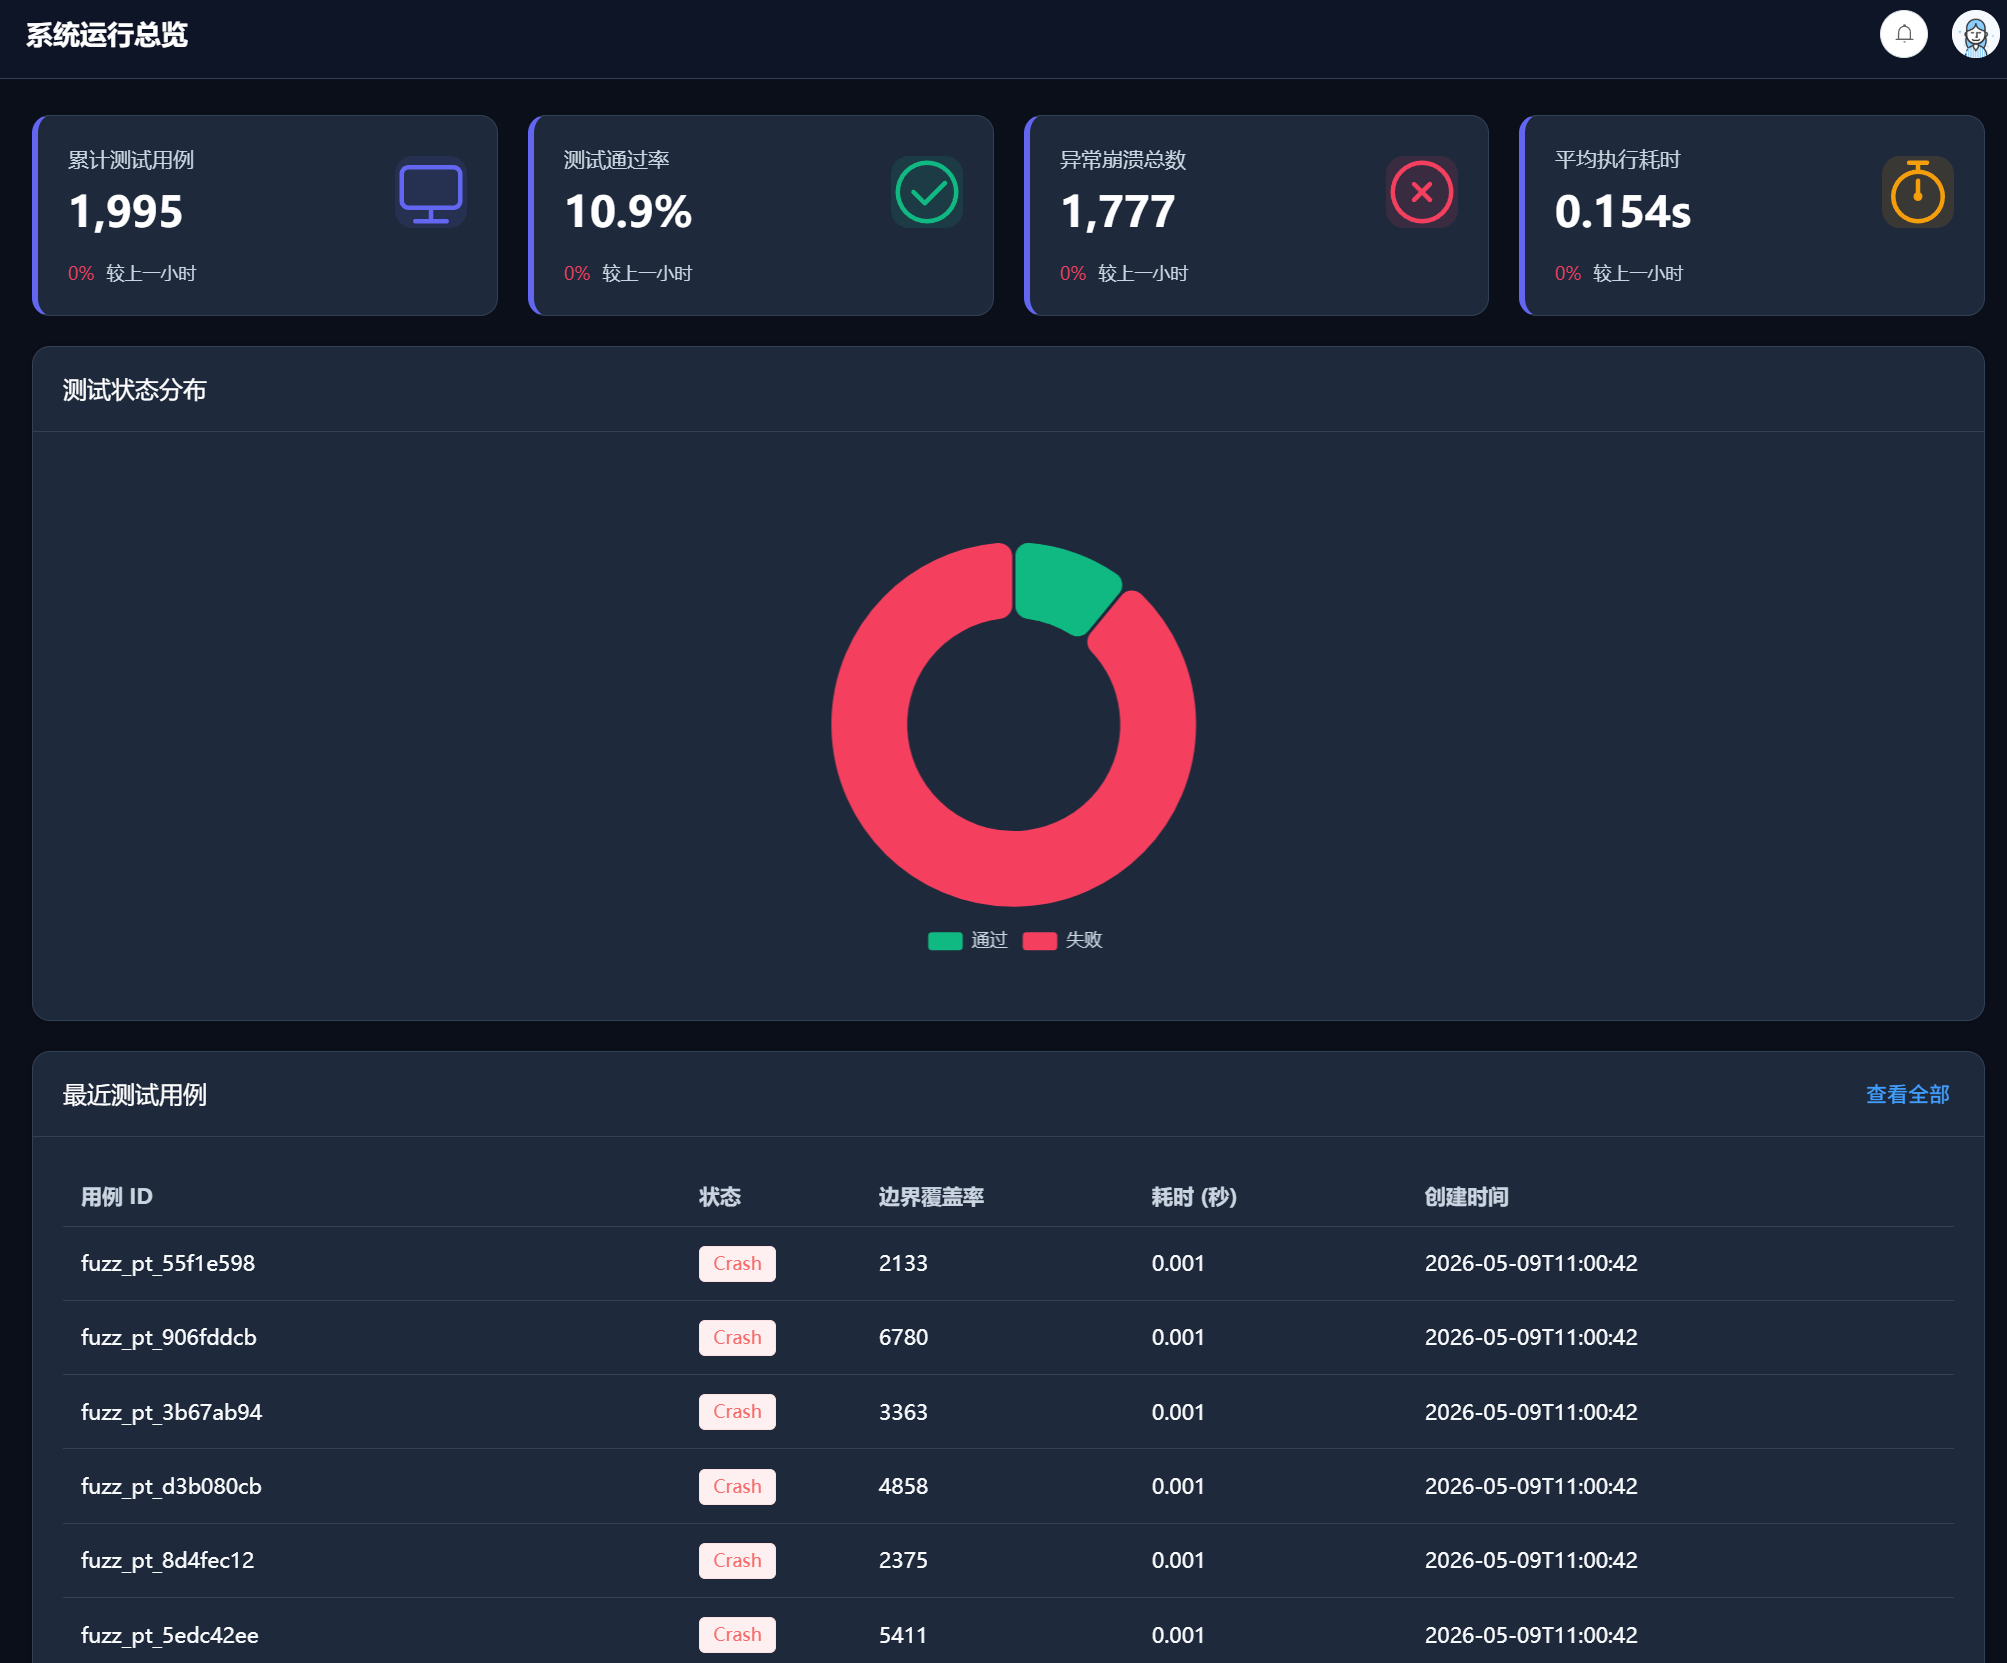
\includegraphics[width=0.75\textwidth]{figure/ui_dashboard.png}
\caption{FuzzHub运行总览界面}
\label{fig:ui_dashboard}
\end{figure}

\subsection{用例管理界面}

用例管理页面用于浏览和筛选测试用例。
用户可以按照执行状态、用例编号等条件查看记录，
也可以进入单条用例的详情页面。
表格中主要展示用例ID、执行状态、覆盖数据、运行耗时和错误摘要等信息。
该页面承担了测试数据入口的作用，
便于用户从大量用例中快速找到需要进一步分析的失败样例。
测试用例管理界面如图\ref{fig:ui_sample_manage}所示。

\begin{figure}[htbp]
\centering
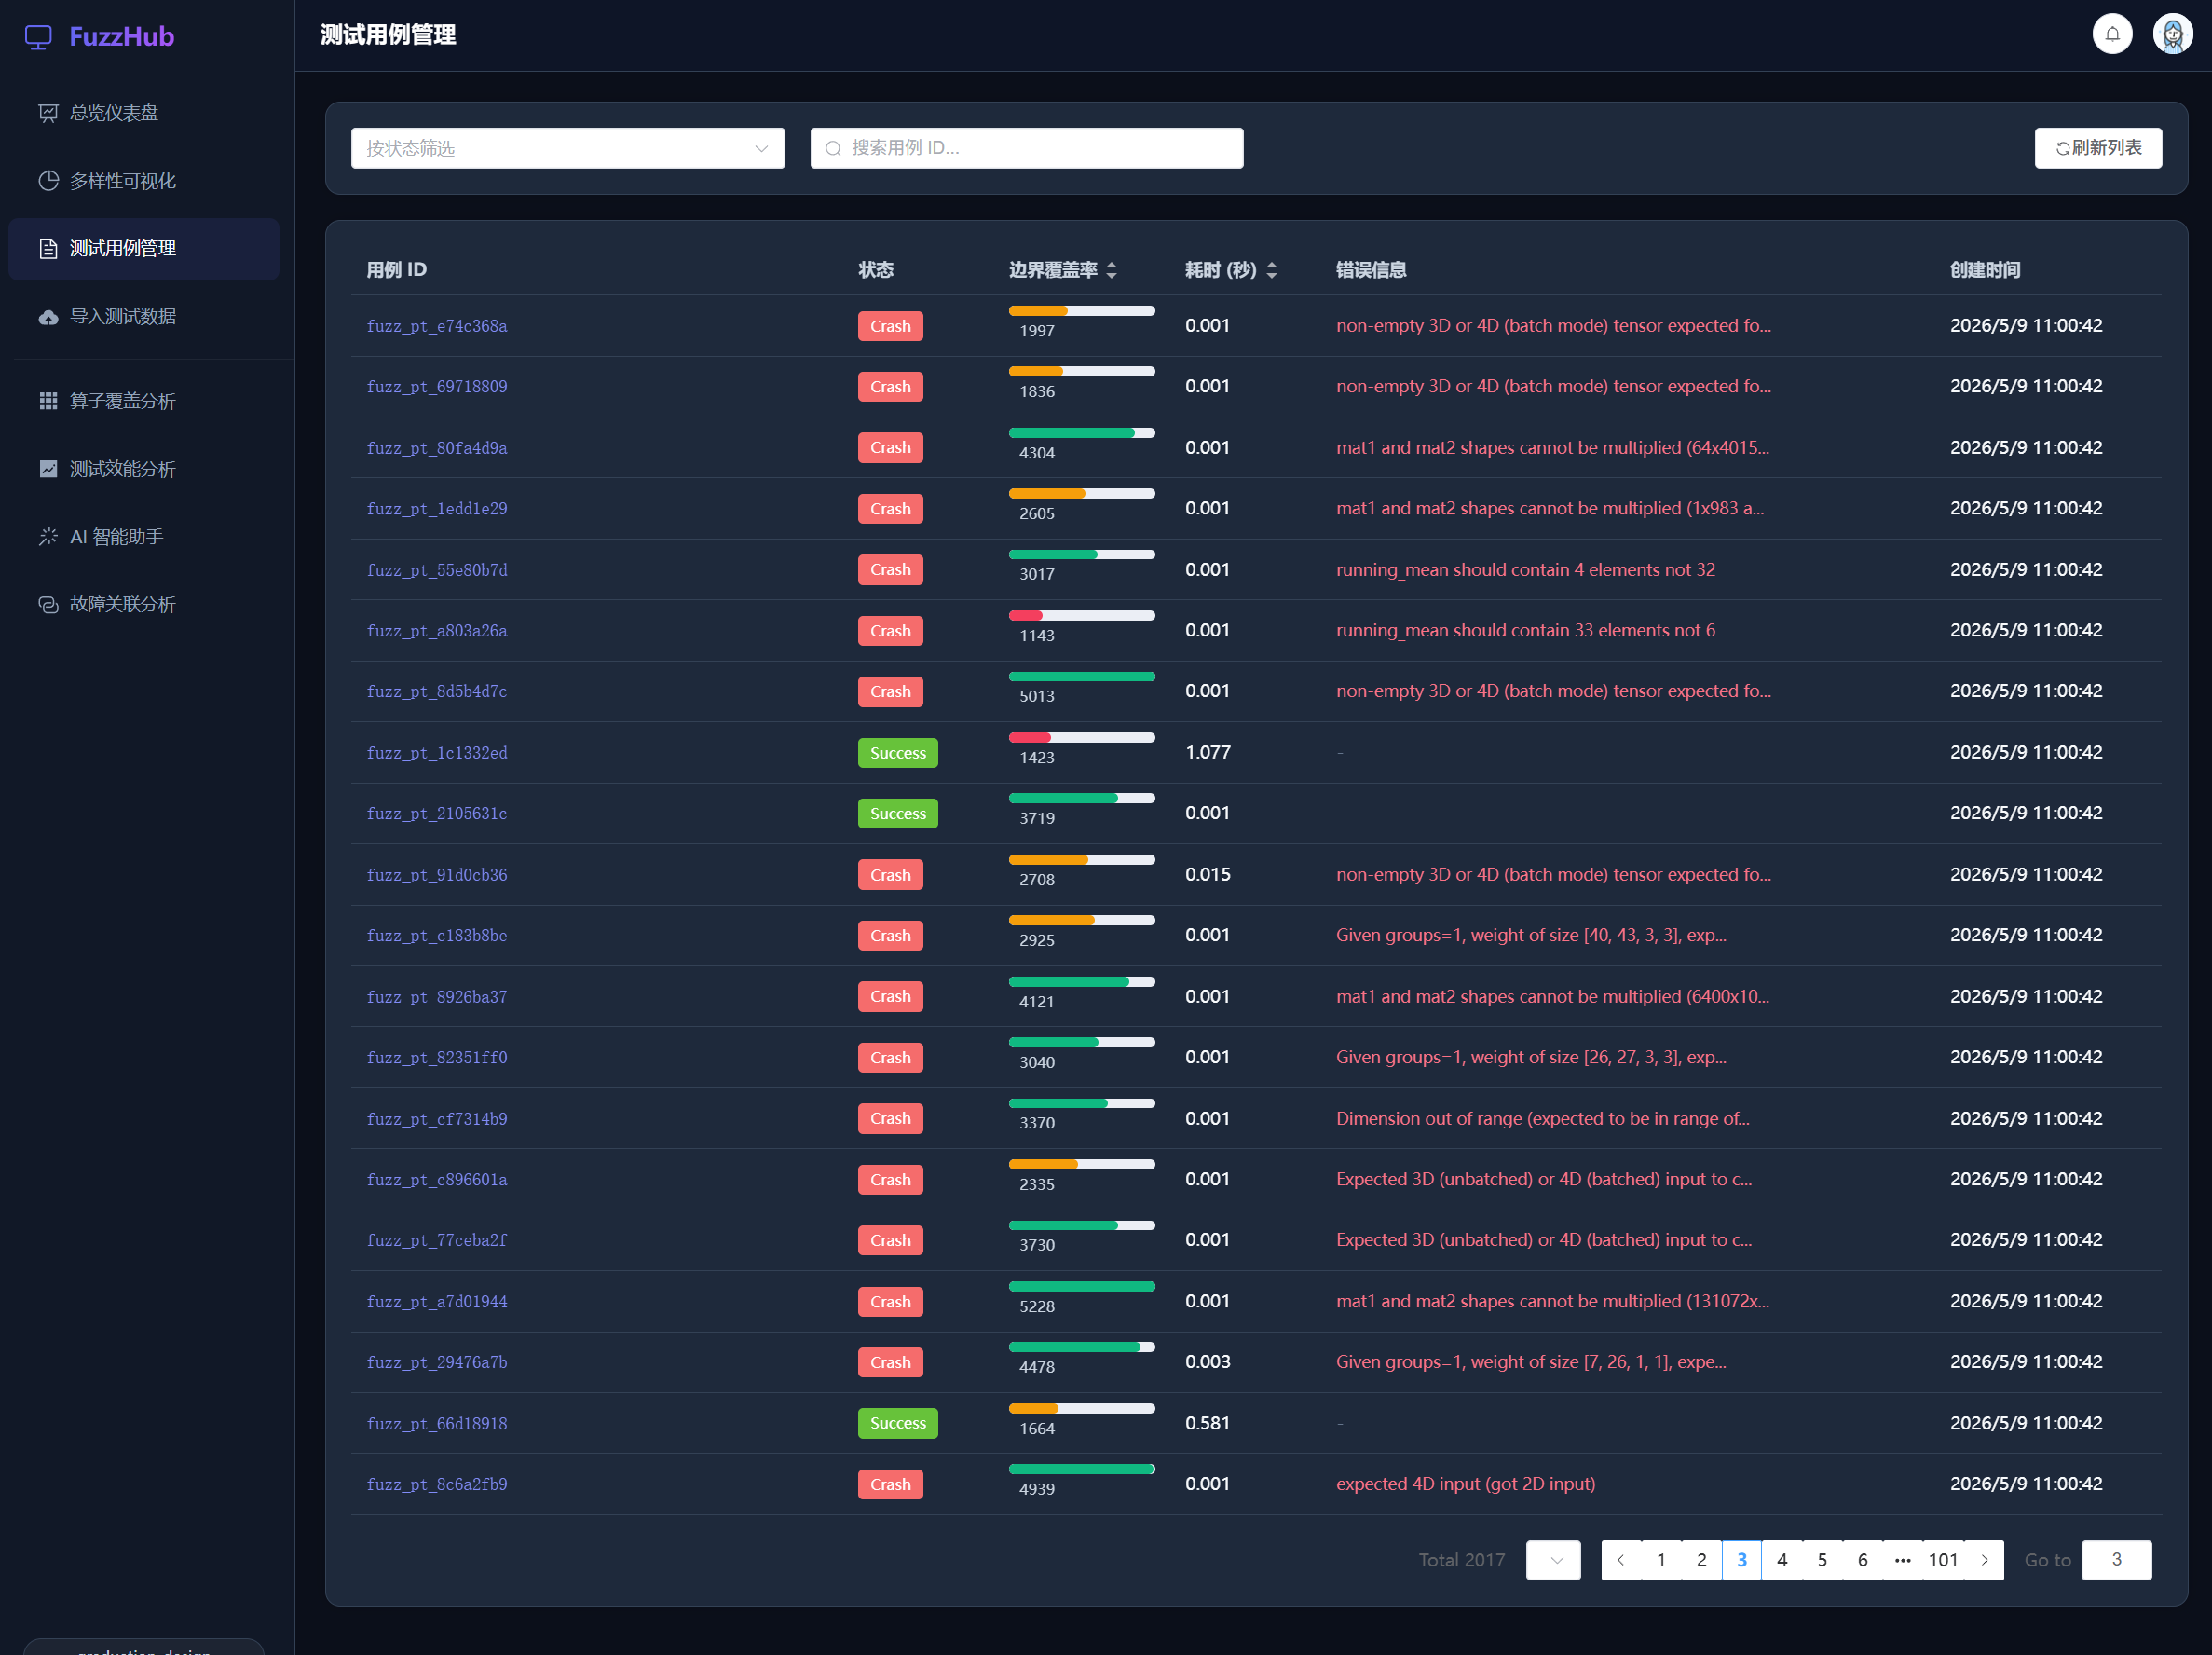
\includegraphics[width=0.75\textwidth]{figure/ui_sample_manage.png}
\caption{测试用例管理界面}
\label{fig:ui_sample_manage}
\end{figure}
\FloatBarrier

\subsection{用例详情故障辅助定位界面}

用例详情界面用于展示单条测试用例的完整信息。
除用例ID、执行状态、运行耗时和覆盖数据外，
页面还会展示错误日志、模型结构和输入参数等内容。
对于失败用例，前端会调用Python后端分析接口，
给出错误类别、候选算子节点和相关说明，
帮助用户缩小排查范围。

该界面还提供候选边界条件分析入口。
用户可以针对某个失败用例发起候选边界条件分析，
查看成功用例与失败用例之间的参数差异，
并生成满足或不满足候选约束的待人工验证样例。
用例详情故障辅助定位界面如图\ref{fig:ui_fault_location}所示。

\begin{figure}[htbp]
\centering
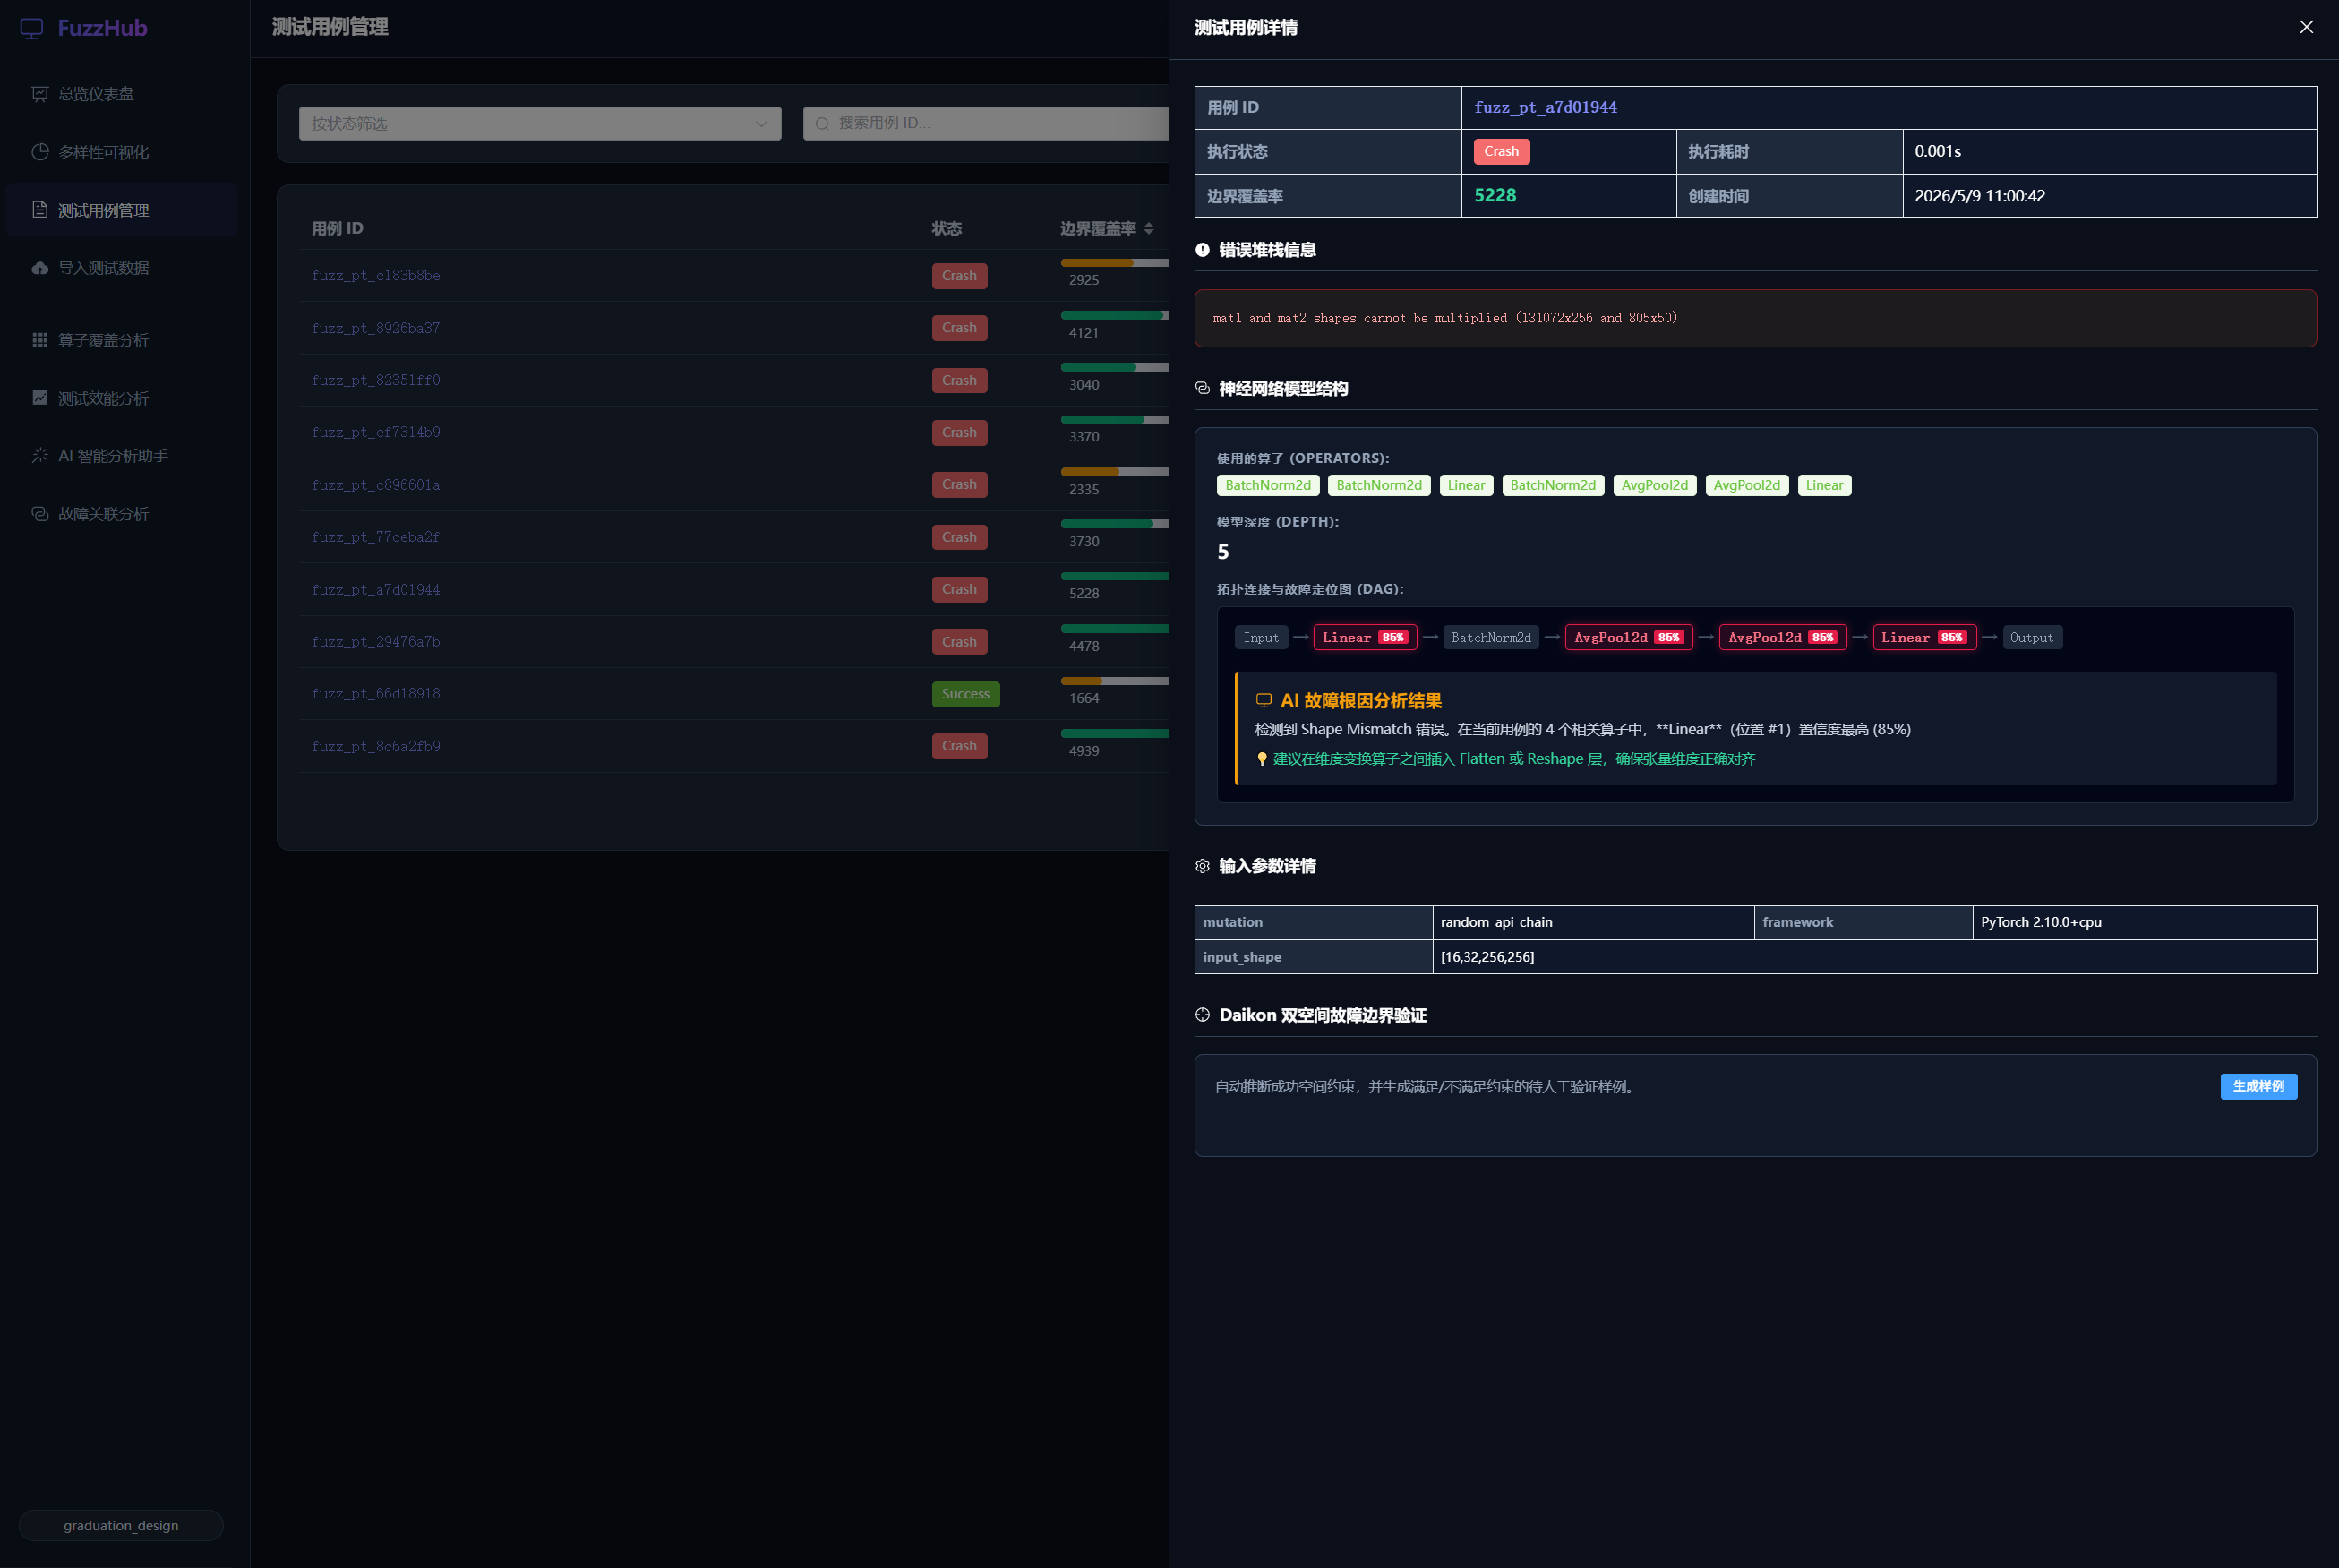
\includegraphics[width=0.75\textwidth]{figure/ui_fault_location.png}
\caption{用例详情故障辅助定位界面}
\label{fig:ui_fault_location}
\end{figure}
\FloatBarrier

\subsection{AI智能分析助手界面}

AI智能分析助手页面用于提供自然语言查询和辅助分析功能。
用户输入问题后，系统会结合历史测试用例进行语义检索，
并生成辅助诊断报告。
页面同时展示相似用例、错误摘要和候选变异建议，
方便用户从已有数据中寻找参考。

该页面主要调用语义问答接口和建议生成接口。
其中，前者用于组织历史相似用例和当前问题上下文，
后者用于给出后续测试方向。
用于辅助开发者进行故障分析和后续测试。
AI智能分析助手界面如图\ref{fig:ui_ai_assistance}所示。

\begin{figure}[htbp]
\centering
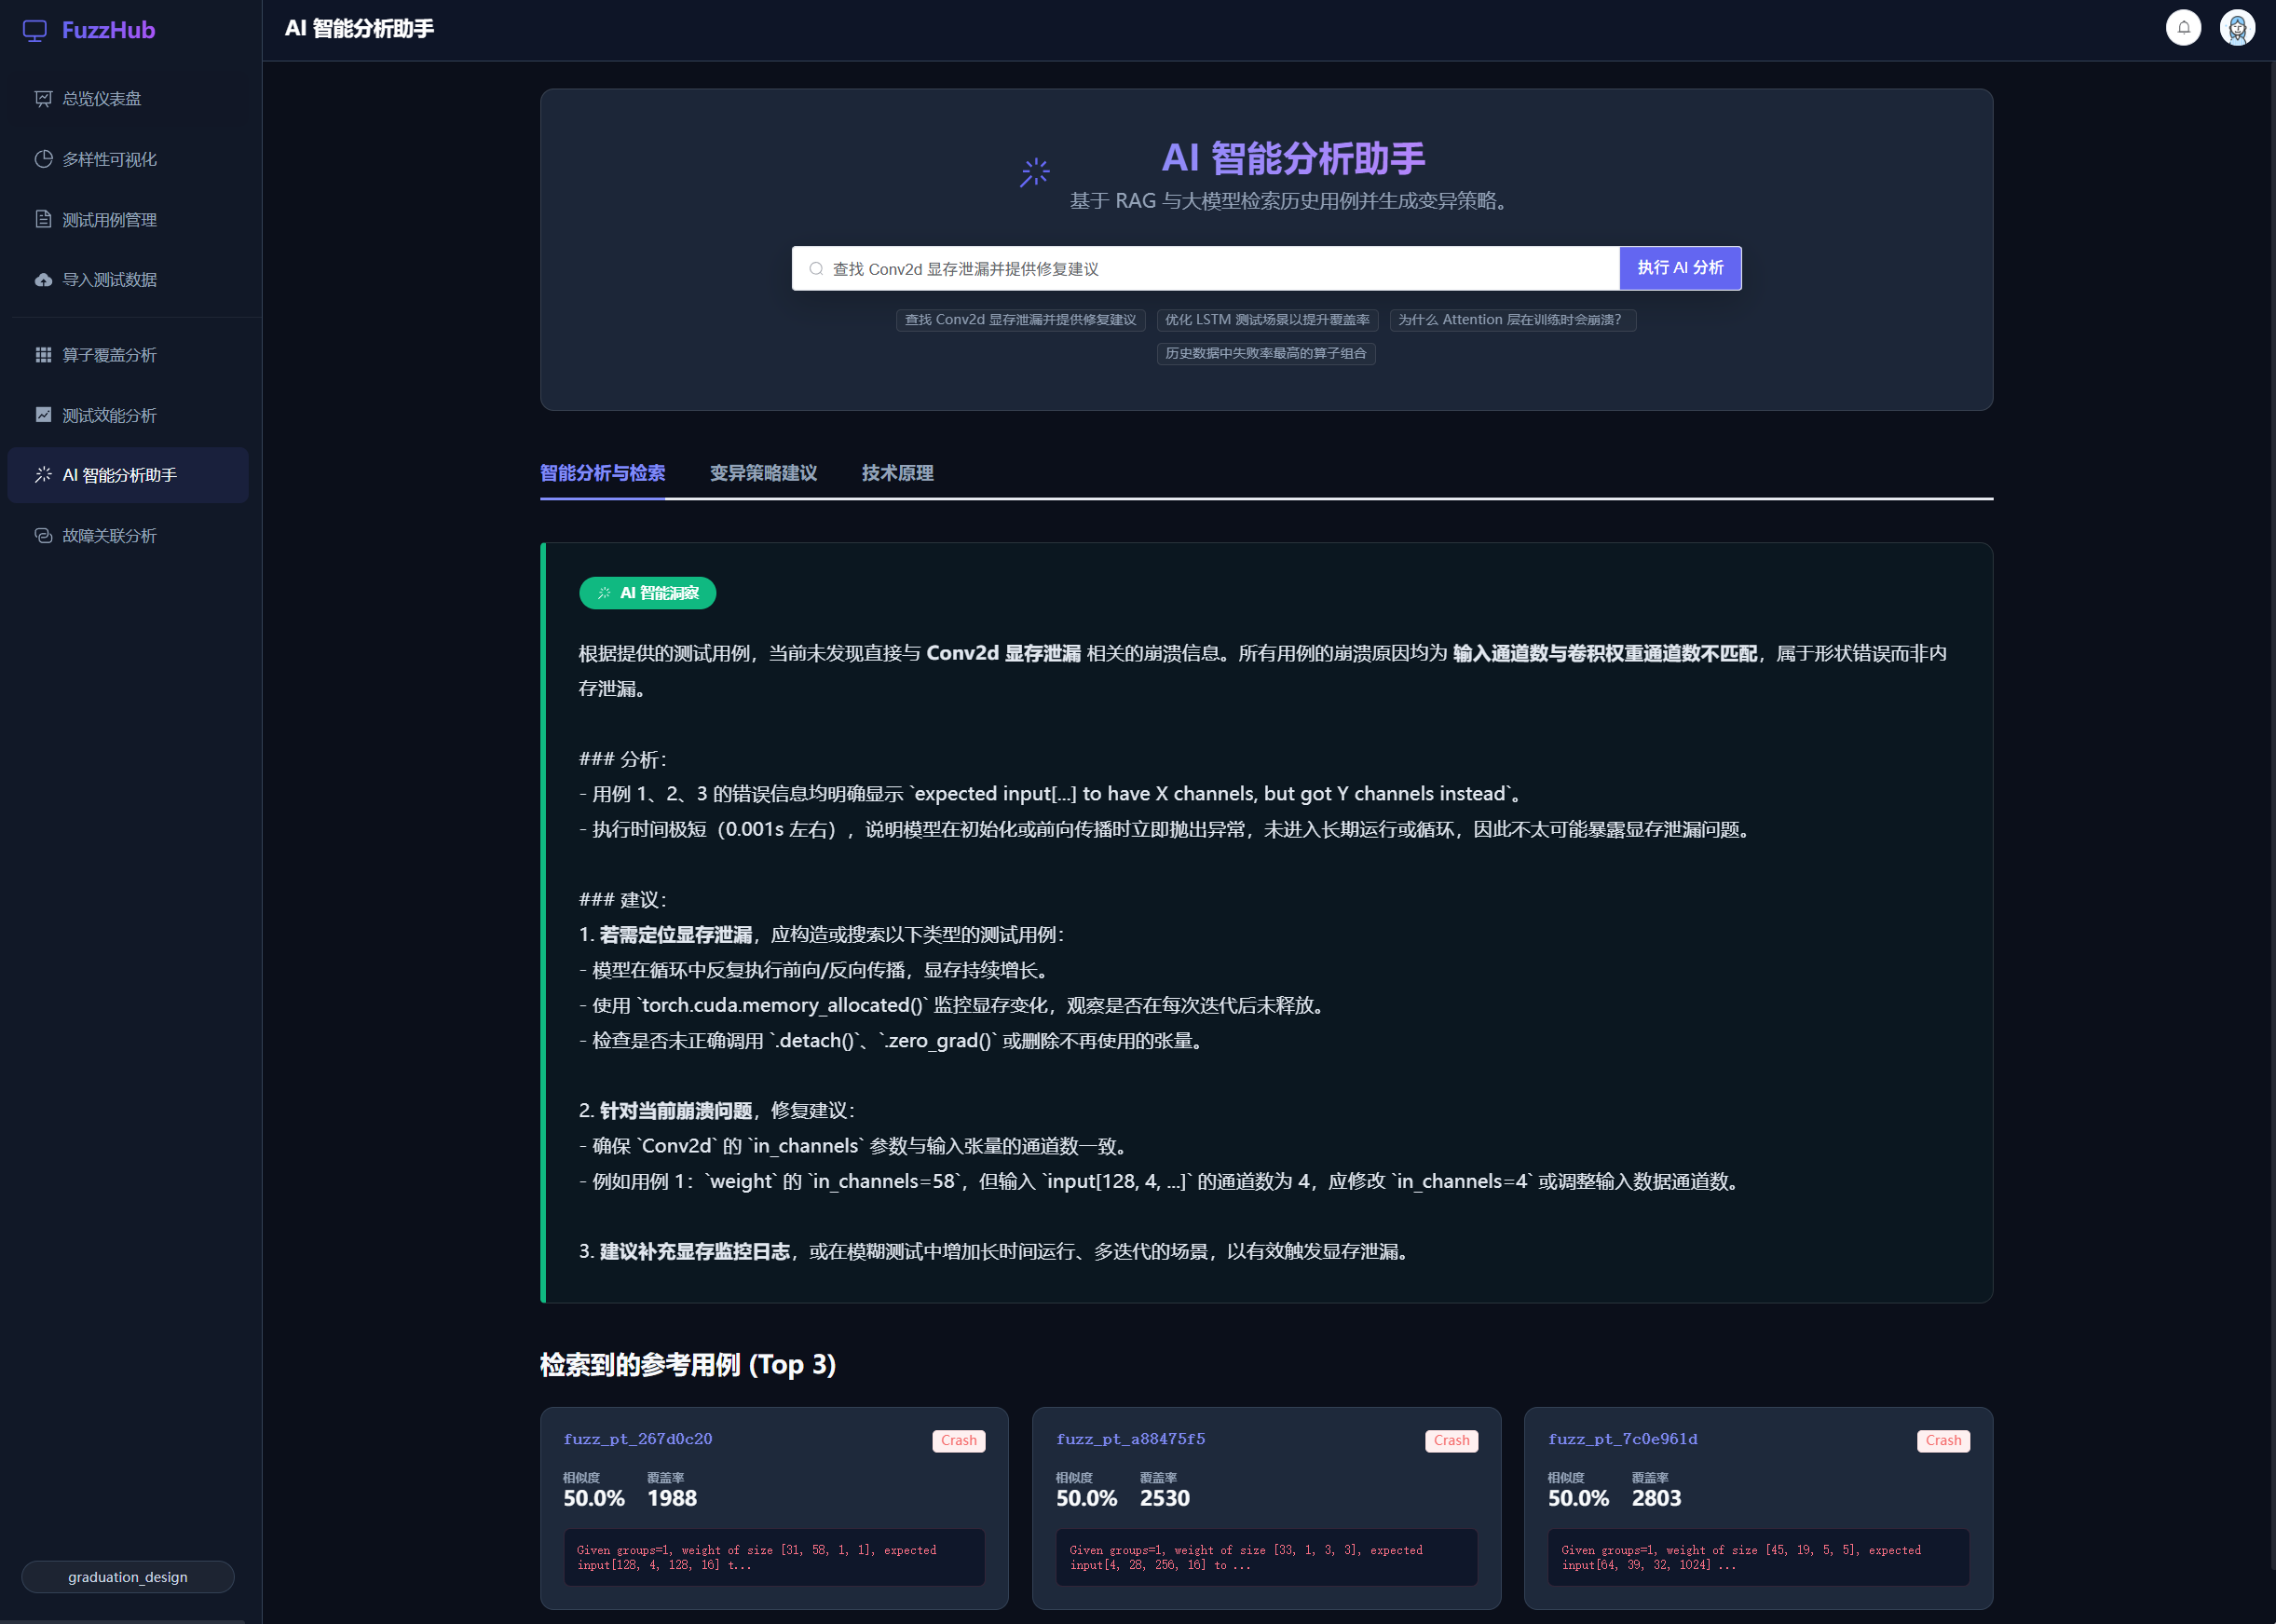
\includegraphics[width=0.75\textwidth]{figure/ui_ai_assistance.png}
\caption{AI智能分析助手界面}
\label{fig:ui_ai_assistance}
\end{figure}
\FloatBarrier

\subsection{故障关联分析界面}

故障关联分析页面用于从整体上查看故障与算子的关系。
页面根据后端返回的故障关联数据，
展示故障用例数量、高风险算子关联和常见错误类型。
中部表格按算子和算子组合汇总故障情况，
便于观察问题是否集中在某些算子或特定连接关系上。
页面还列出部分个案级故障记录，
用户可以从中选择失败用例继续进行边界对比分析。
“故障关联分析”页面如图\ref{fig:ui_fault_analysis}所示。

\begin{figure}[htbp]
\centering
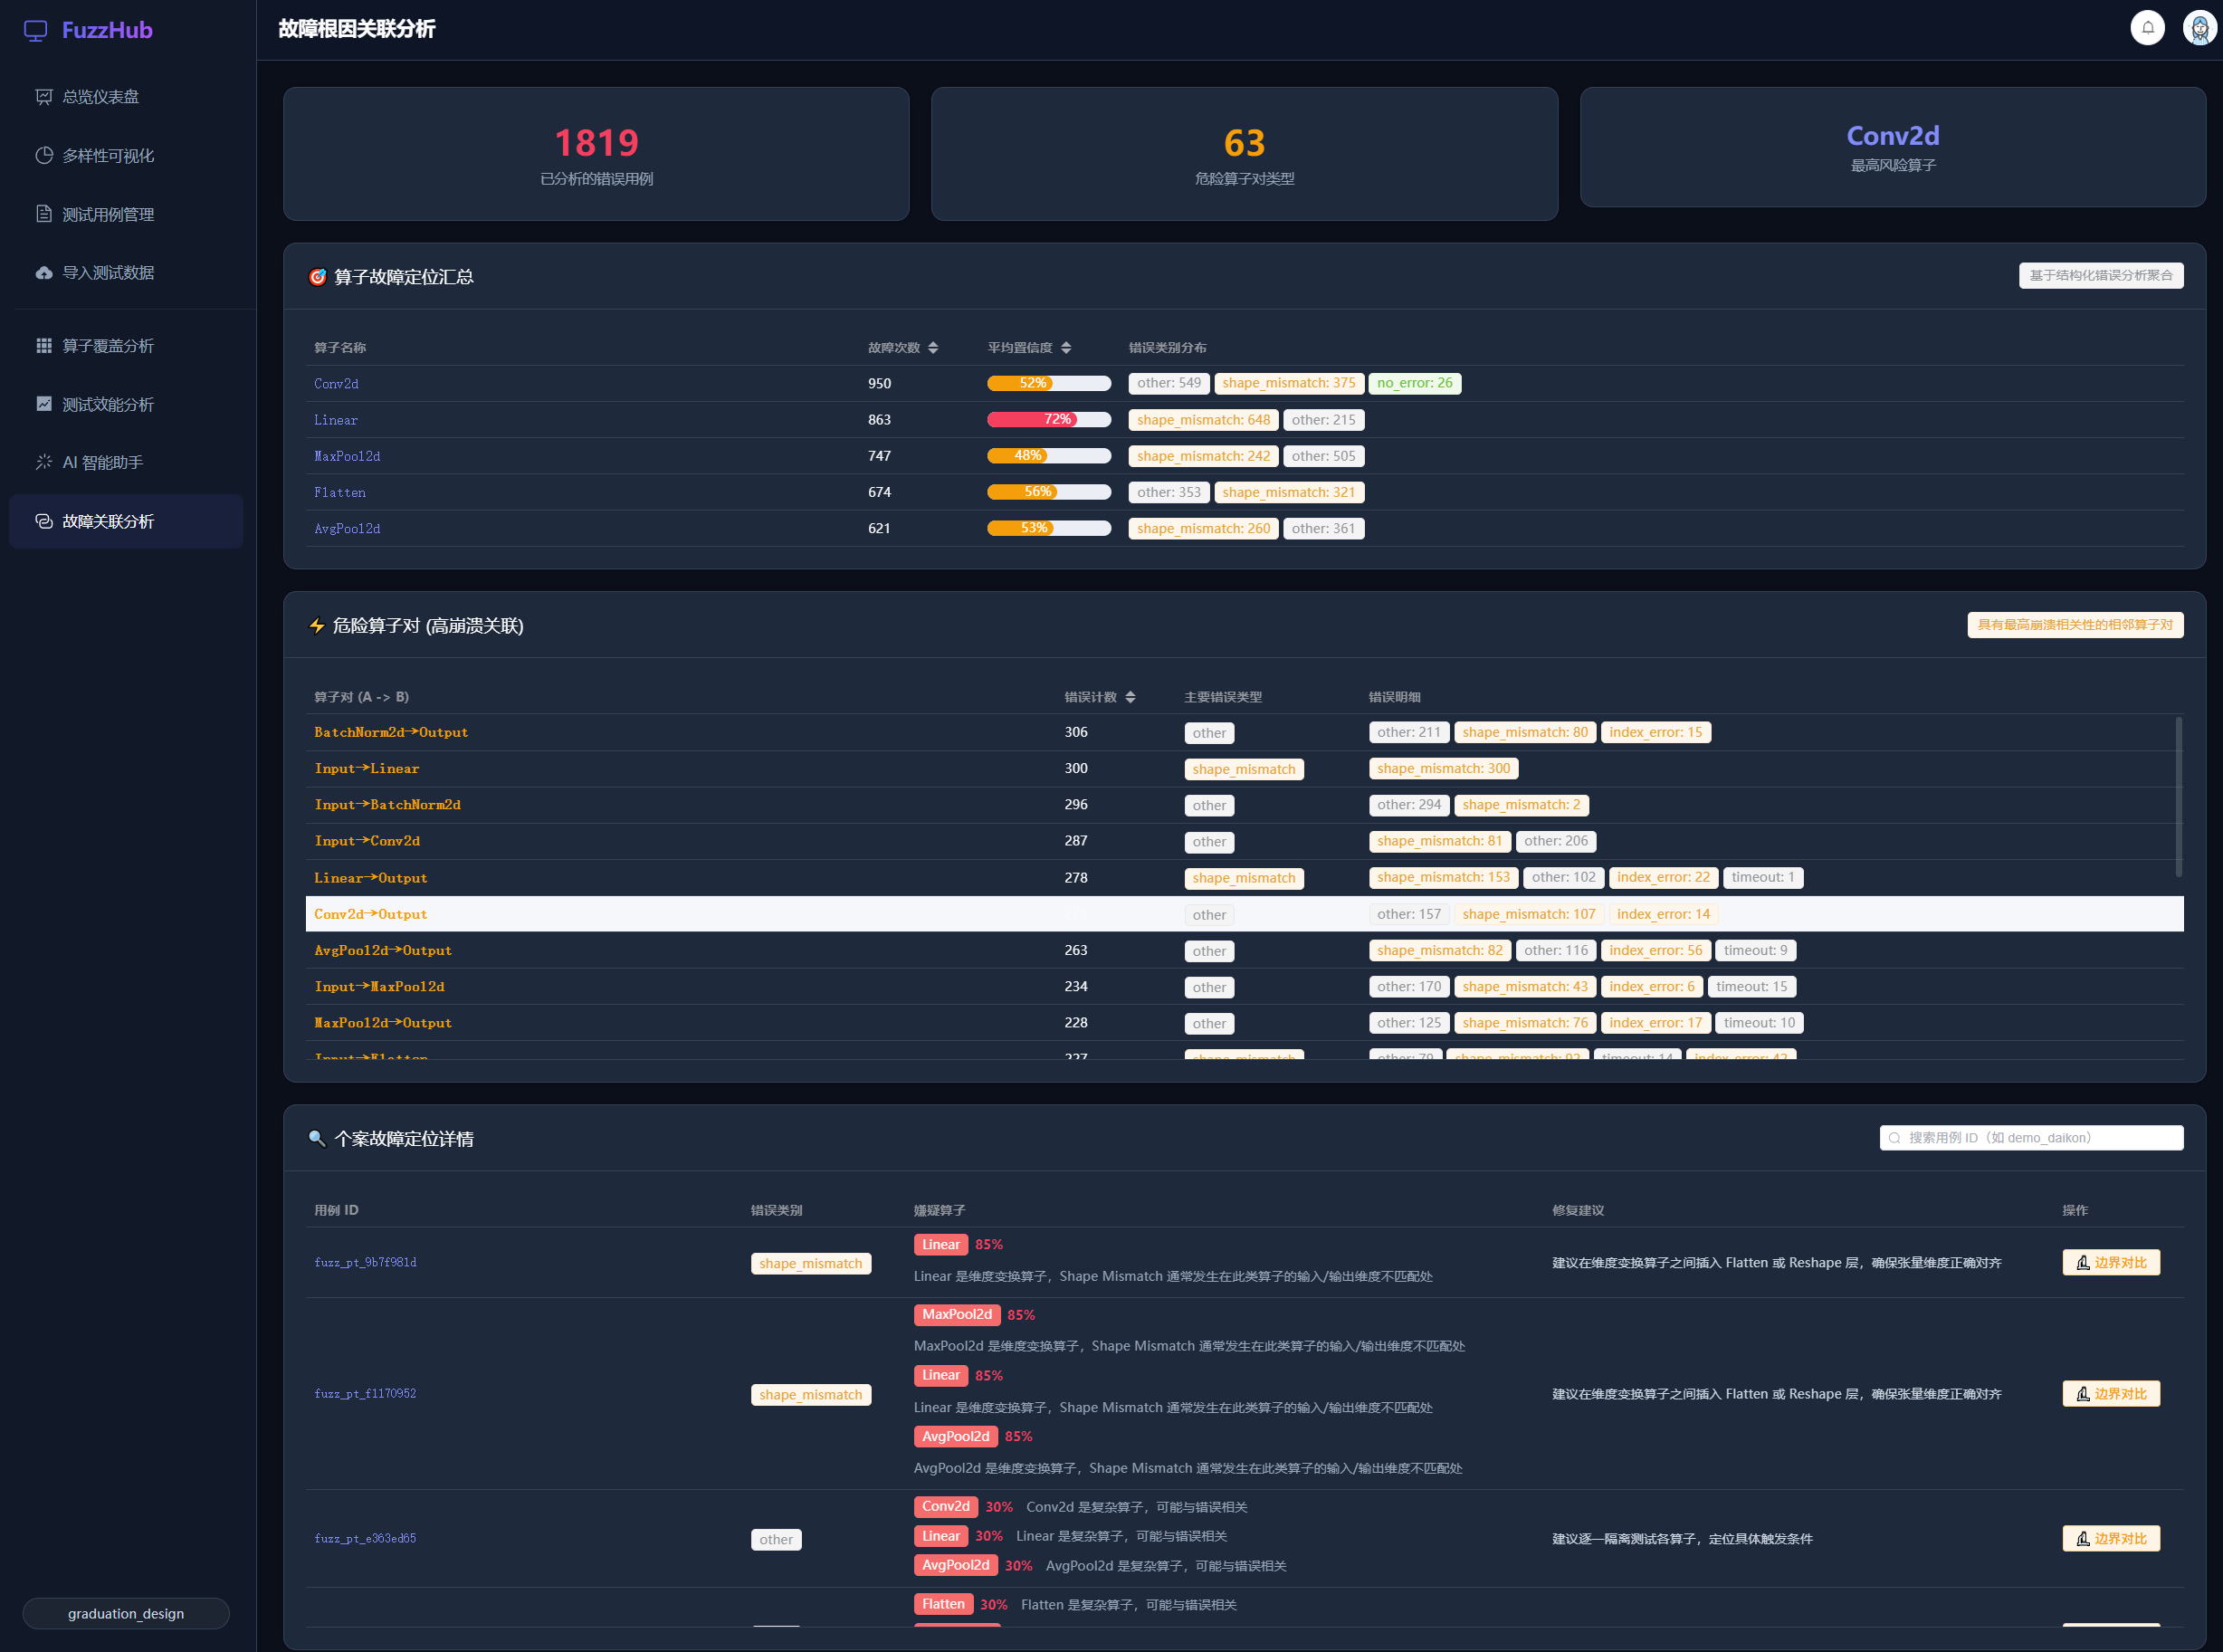
\includegraphics[width=0.75\textwidth]{figure/ui_fault_analysis.png}
\caption{故障关联分析}
\label{fig:ui_fault_analysis}
\end{figure}

边界对比弹窗用于展示单个失败用例与相近成功用例之间的差异。
弹窗中同时展示参数差分、Daikon候选约束、验证样例和辅助诊断报告。
其中，候选约束用于提示可能存在的参数边界，
验证样例则分为满足约束和违反约束两类，
作为后续补充测试和验证边界条件的参考。
界面会标记这些样例仍处于待人工验证状态，
避免把生成结果直接解释为已经执行通过或失败。
底部的辅助诊断报告用于解释候选边界条件。
故障临界差分对比弹窗如图\ref{fig:ui_daikon}所示。

\begin{figure}[htbp]
\centering
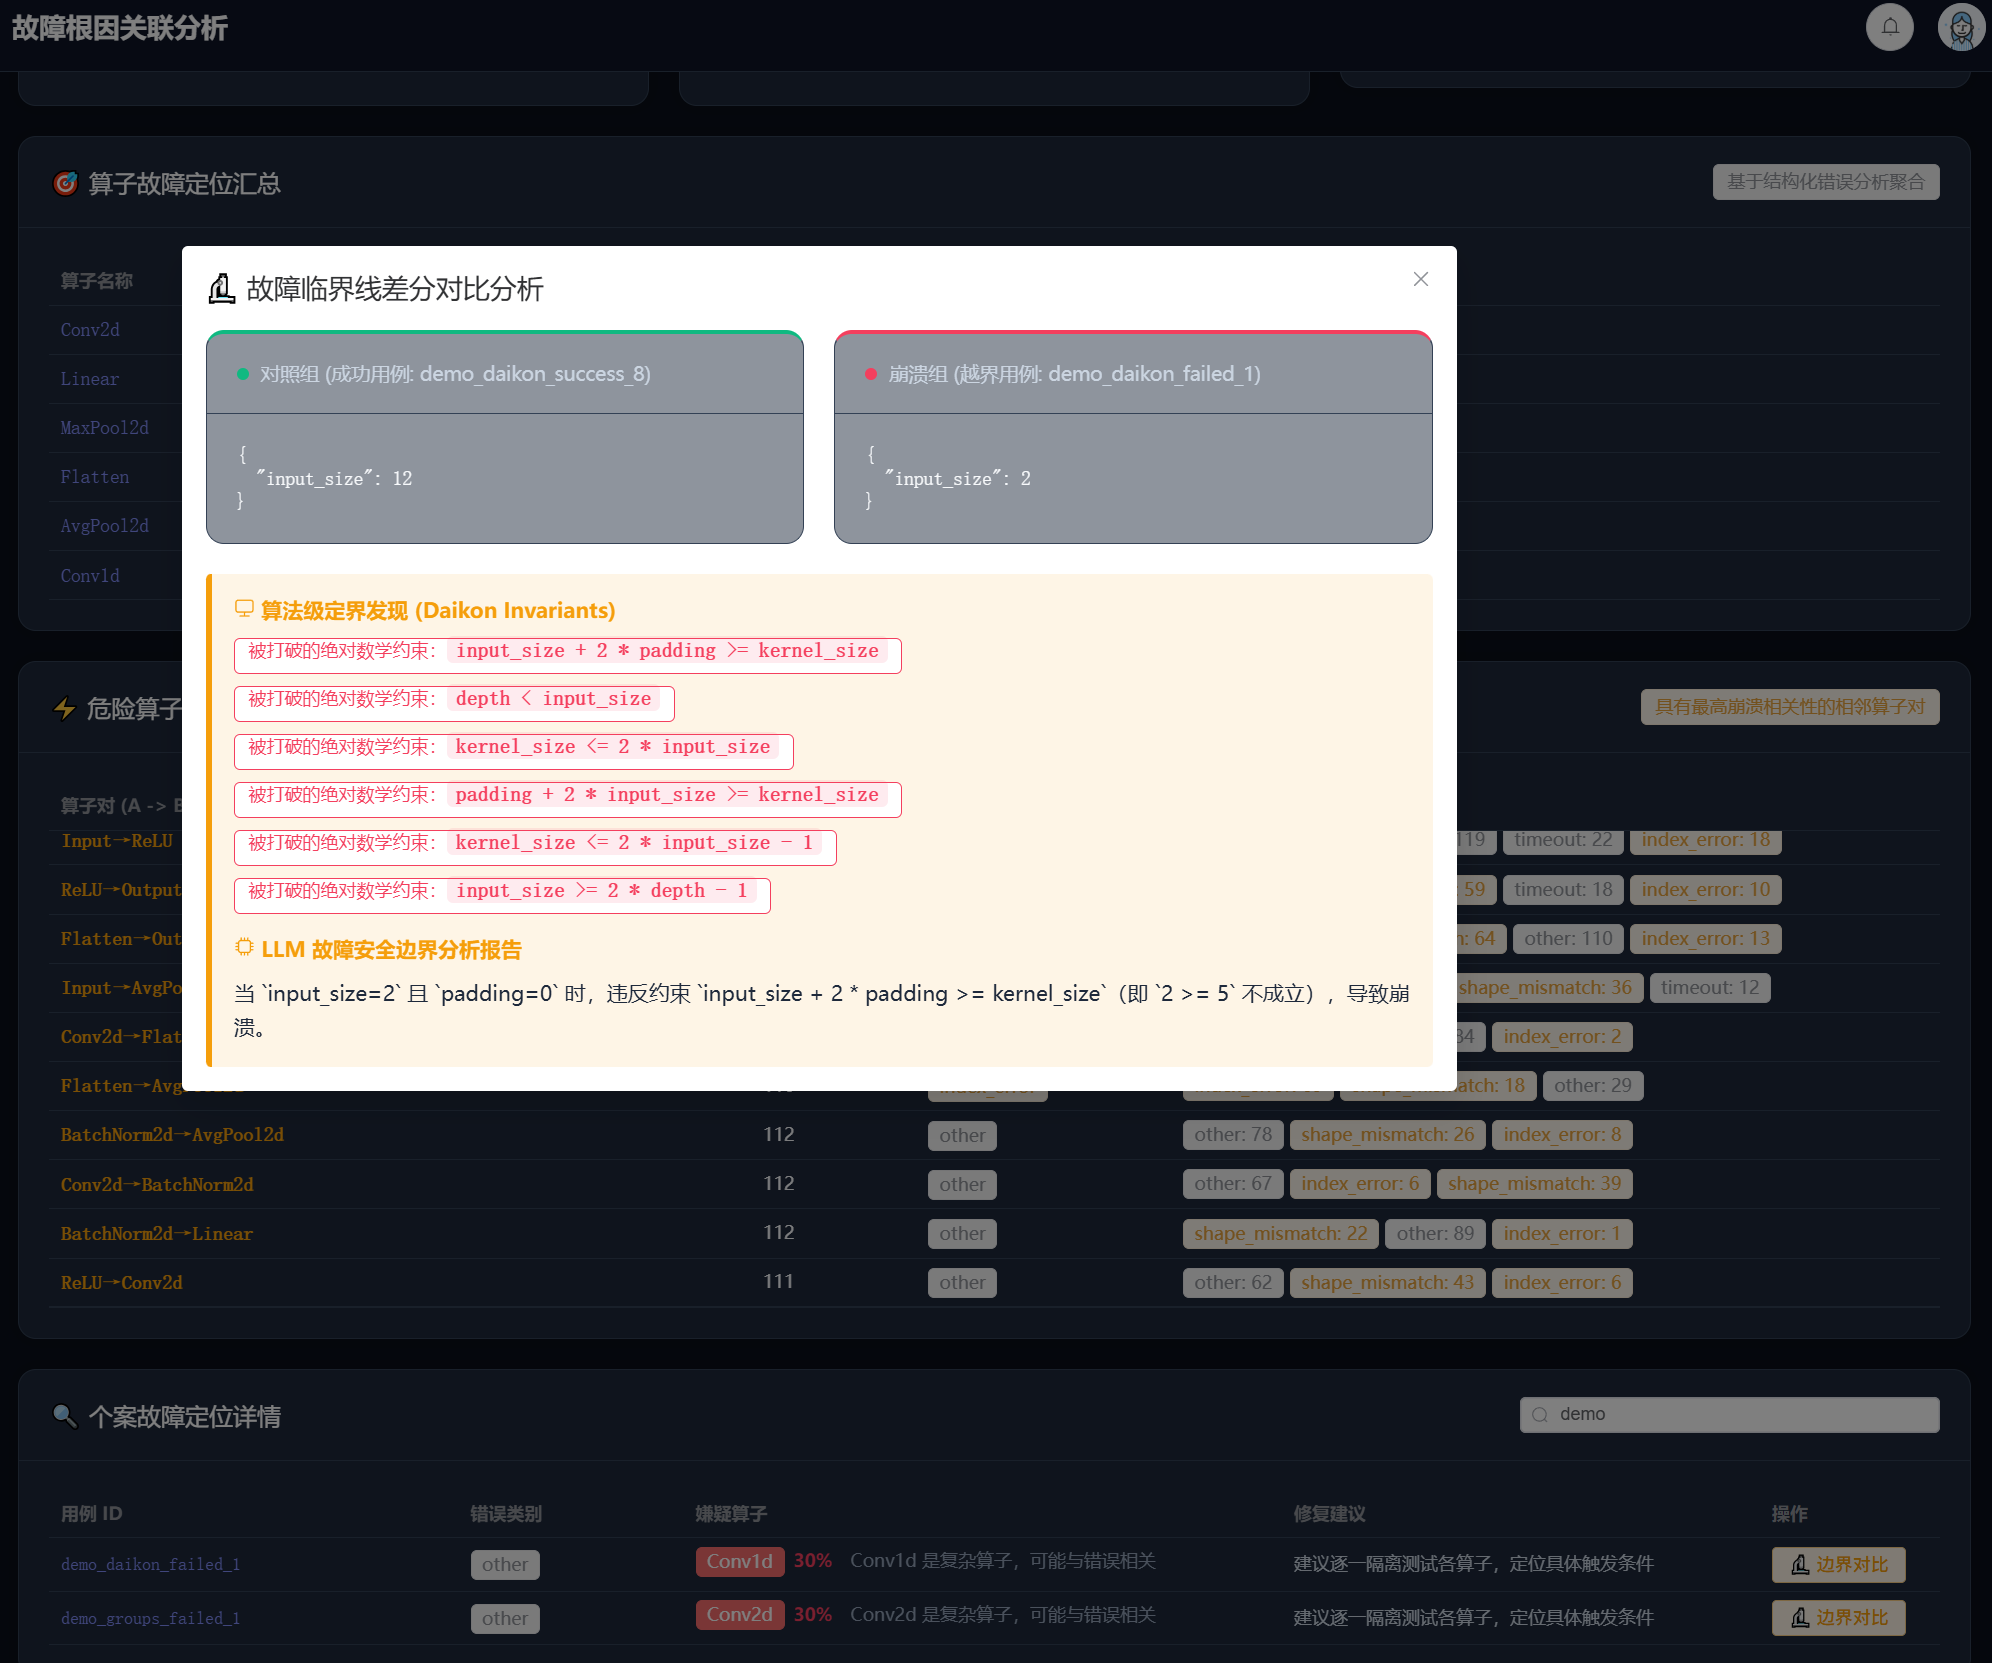
\includegraphics[width=0.75\textwidth]{figure/ui_daikon.png}
\caption{故障临界差分对比}
\label{fig:ui_daikon}
\end{figure}
\FloatBarrier

\subsection{算子覆盖缺口分析界面}

算子覆盖缺口分析页面用于查看当前测试集对算子和算子组合的覆盖情况。
页面通过覆盖缺口分析接口获取统计结果，
并以统计卡片、热力图和表格的形式展示。
用户可以看到哪些算子已经被测试覆盖，
哪些算子对在现有用例中还没有出现。
这部分信息为后续补充测试提供了直接依据。
算子覆盖缺口分析界面如图\ref{fig:ui_coverage}所示。

\begin{figure}[htbp]
\centering
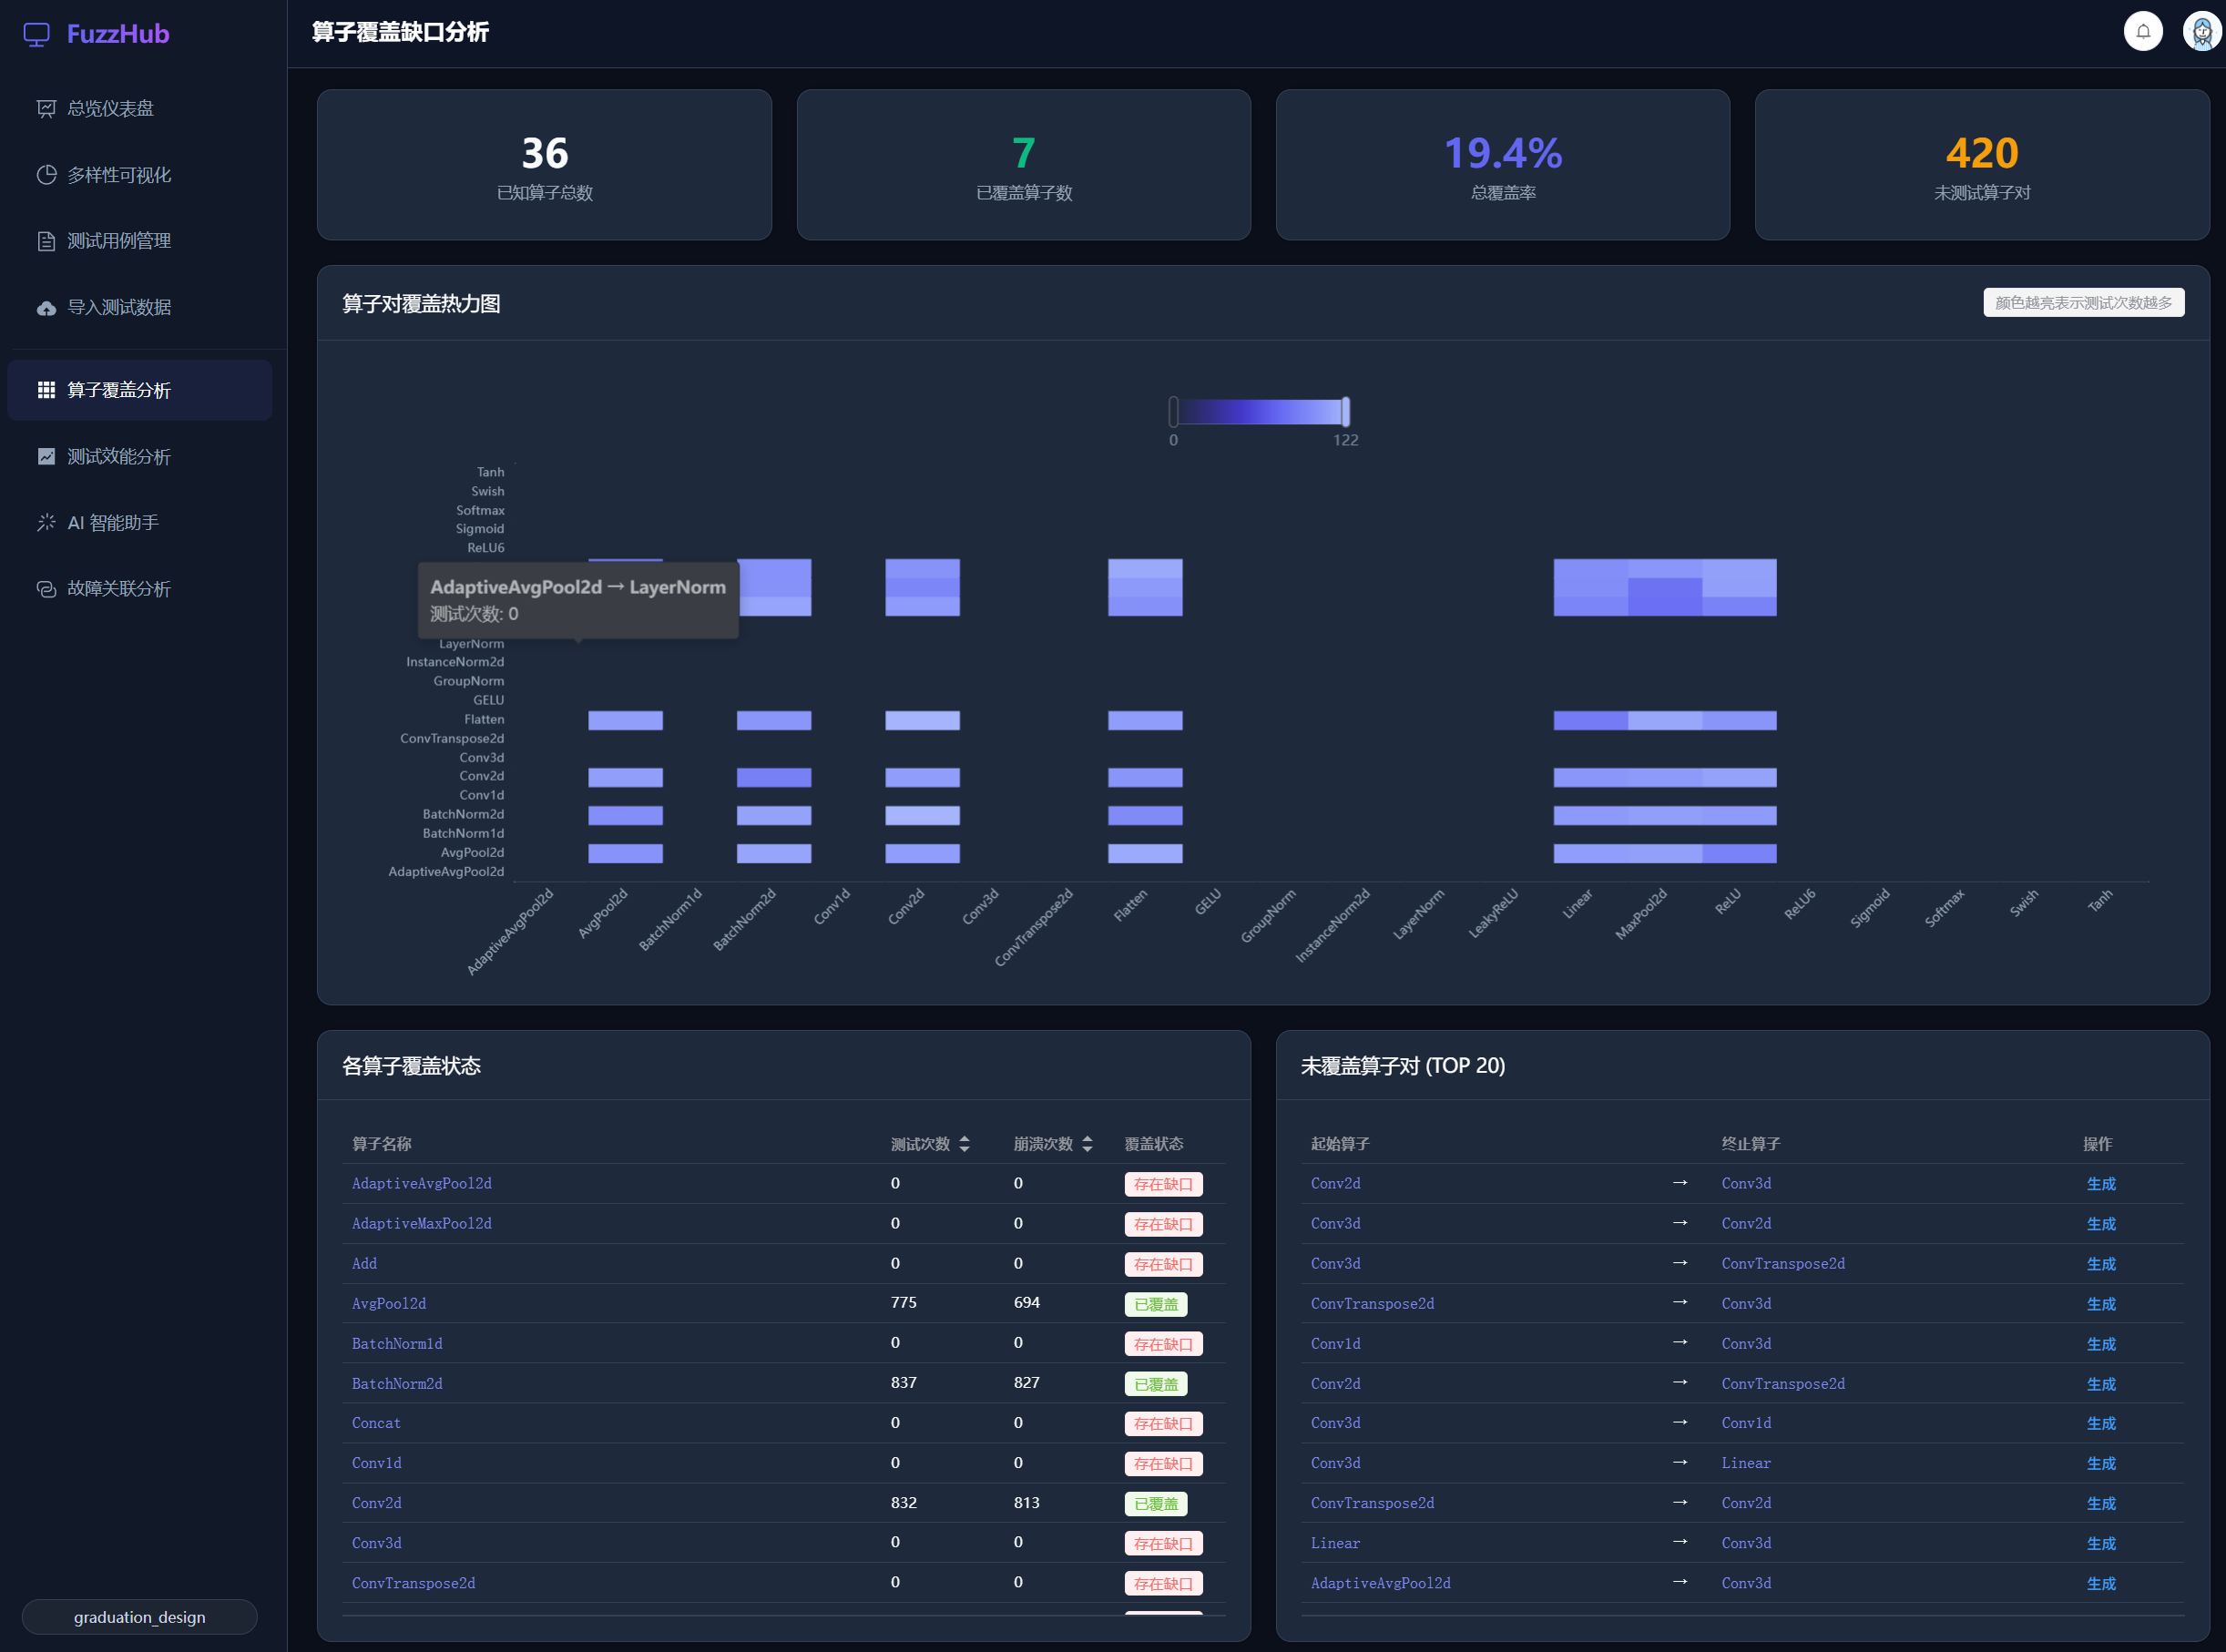
\includegraphics[width=0.75\textwidth]{figure/ui_coverage.png}
\caption{算子覆盖缺口分析界面}
\label{fig:ui_coverage}
\end{figure}

对于未覆盖的算子组合，页面提供候选补盲测试脚本生成入口。
用户选择目标算子对后，
前端调用候选补盲生成接口生成候选脚本。
生成结果会在弹窗中展示，
用户可以据此检查脚本是否可运行、是否具有覆盖贡献以及是否适合后续入库。
AI定向补盲生成结果界面如图\ref{fig:ui_coverage_blind}所示。

\begin{figure}[htbp]
\centering
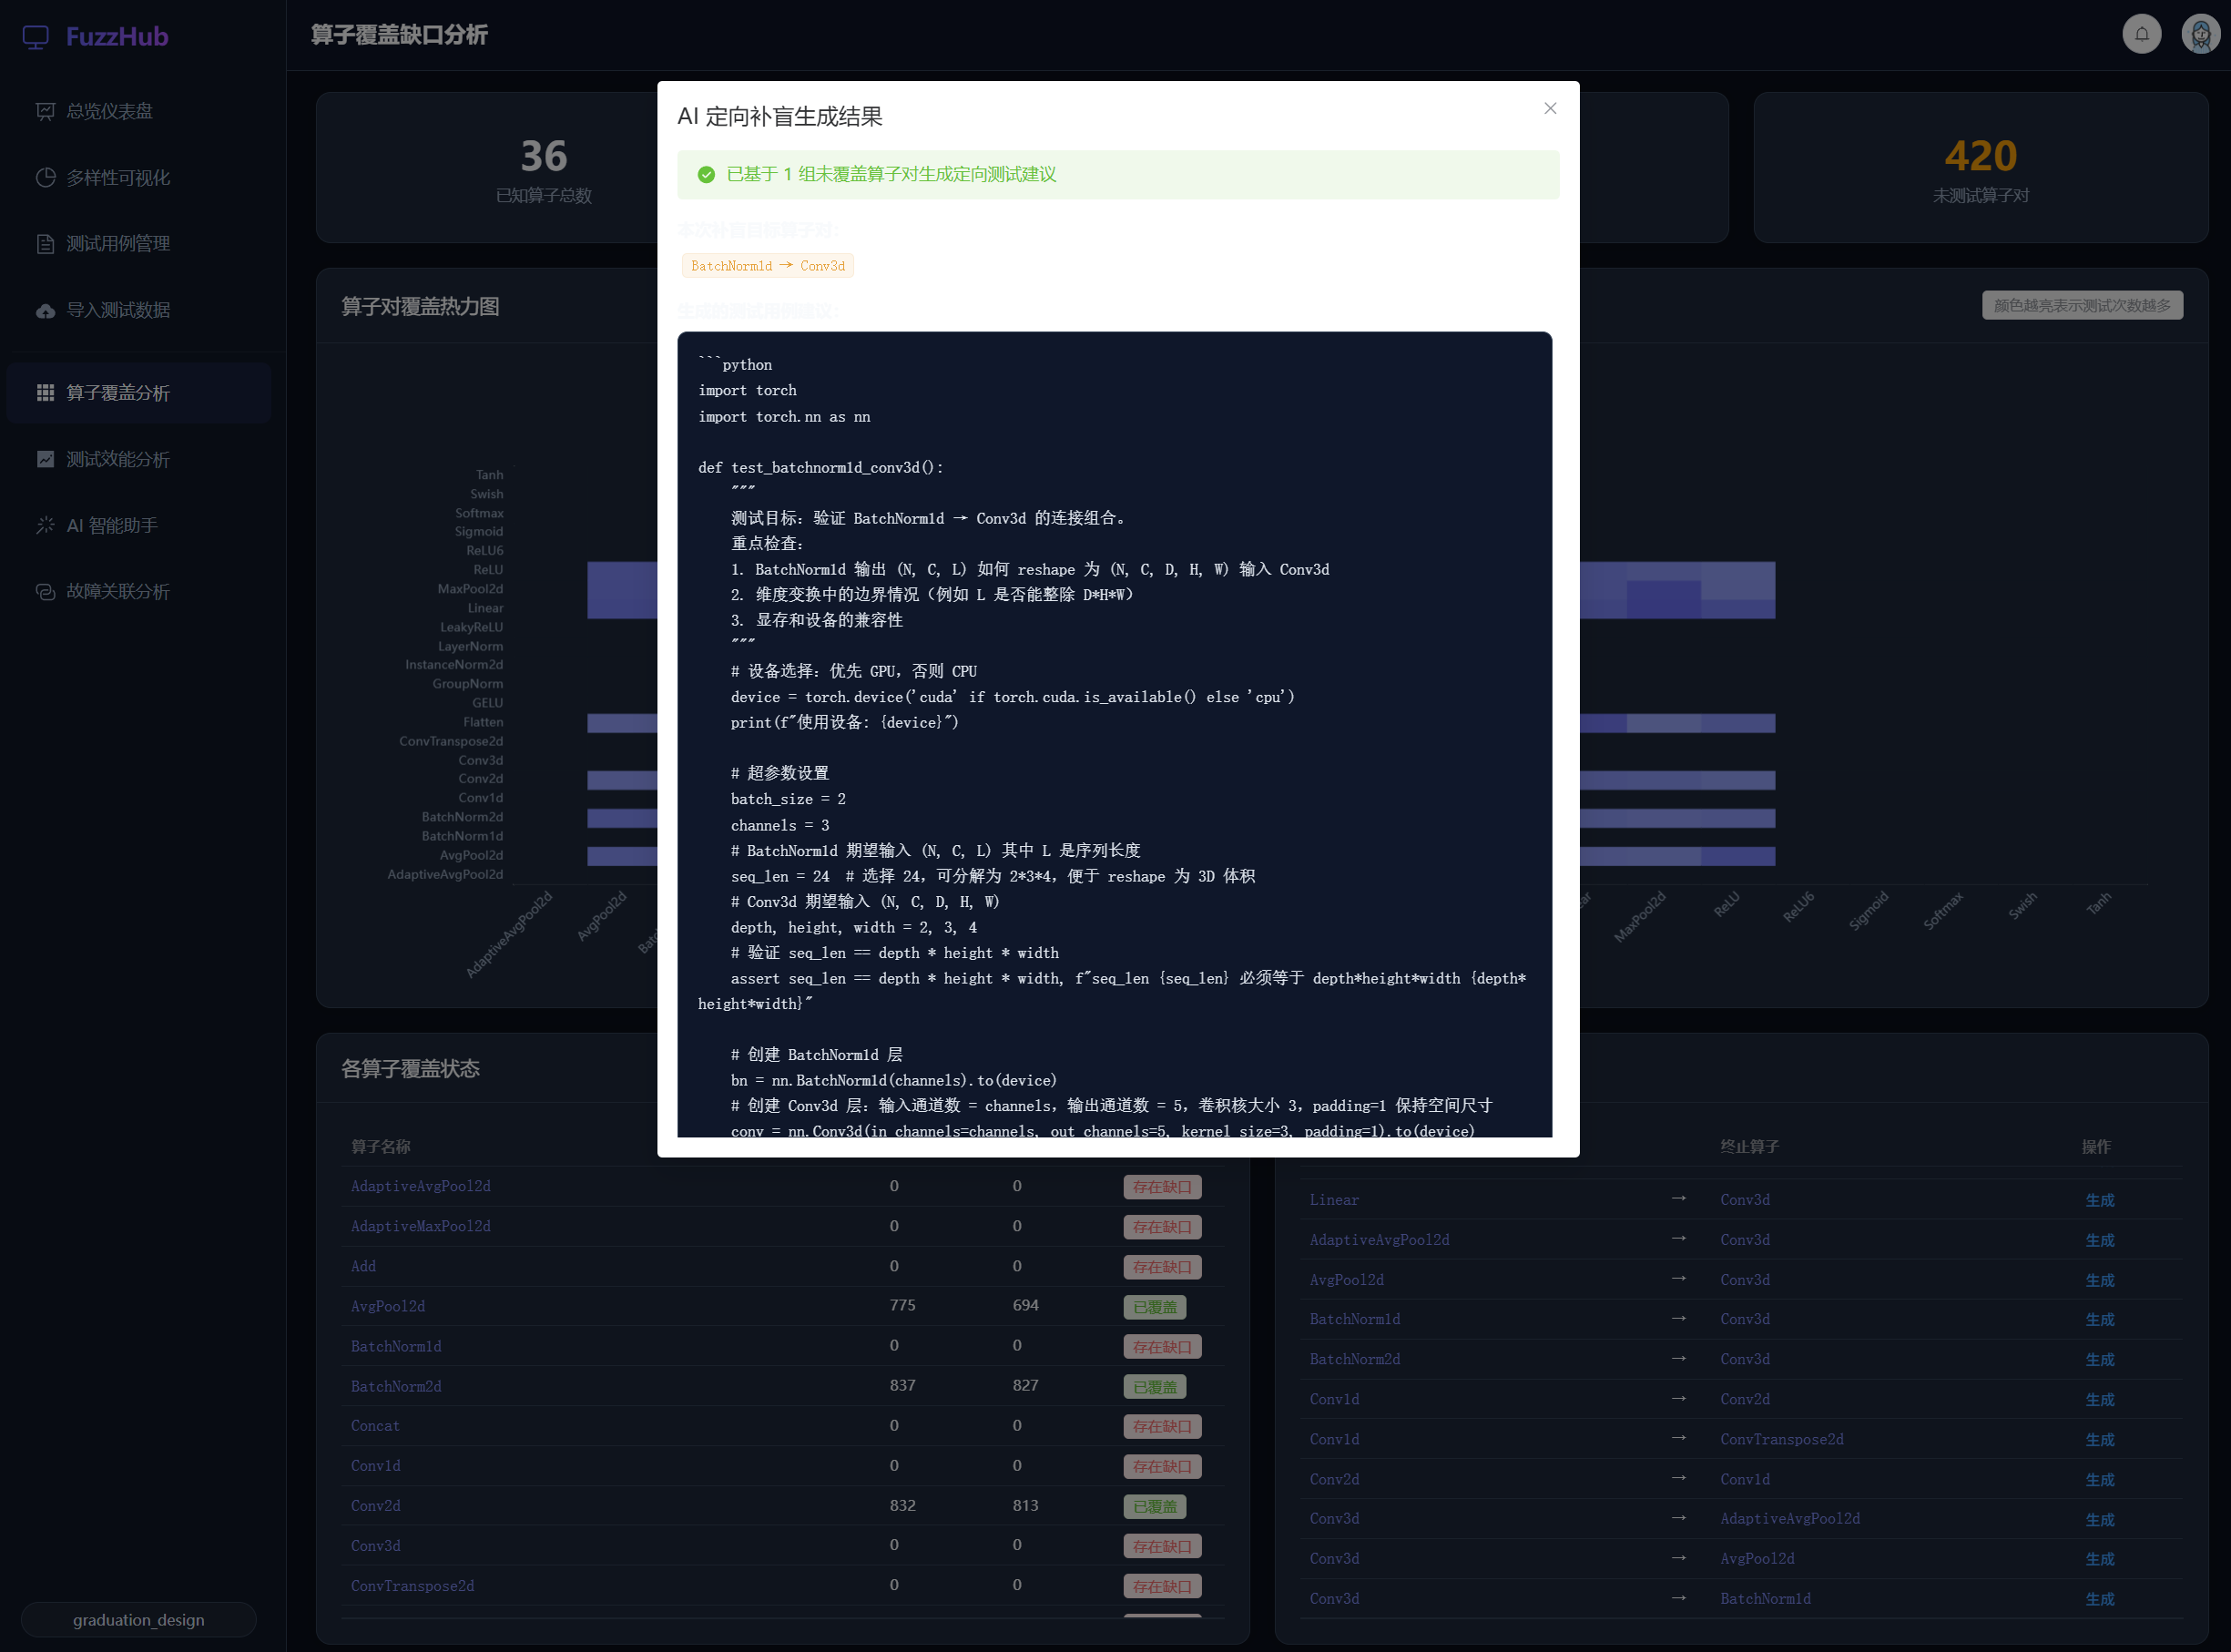
\includegraphics[width=0.75\textwidth]{figure/ui_coverage_blind.png}
\caption{AI定向补盲生成结果界面}
\label{fig:ui_coverage_blind}
\end{figure}
\FloatBarrier

\subsection{测试效能评估界面}

测试效能评估页面用于展示CEI指标、用例效能排行和清退方案，
帮助用户区分优先保留用例和候选清退用例。
用户可以先预览阈值清退结果，确认后再执行处理。
测试效能评估界面如图\ref{fig:ui_efficiency_scatter}所示。

\begin{figure}[H]
\centering
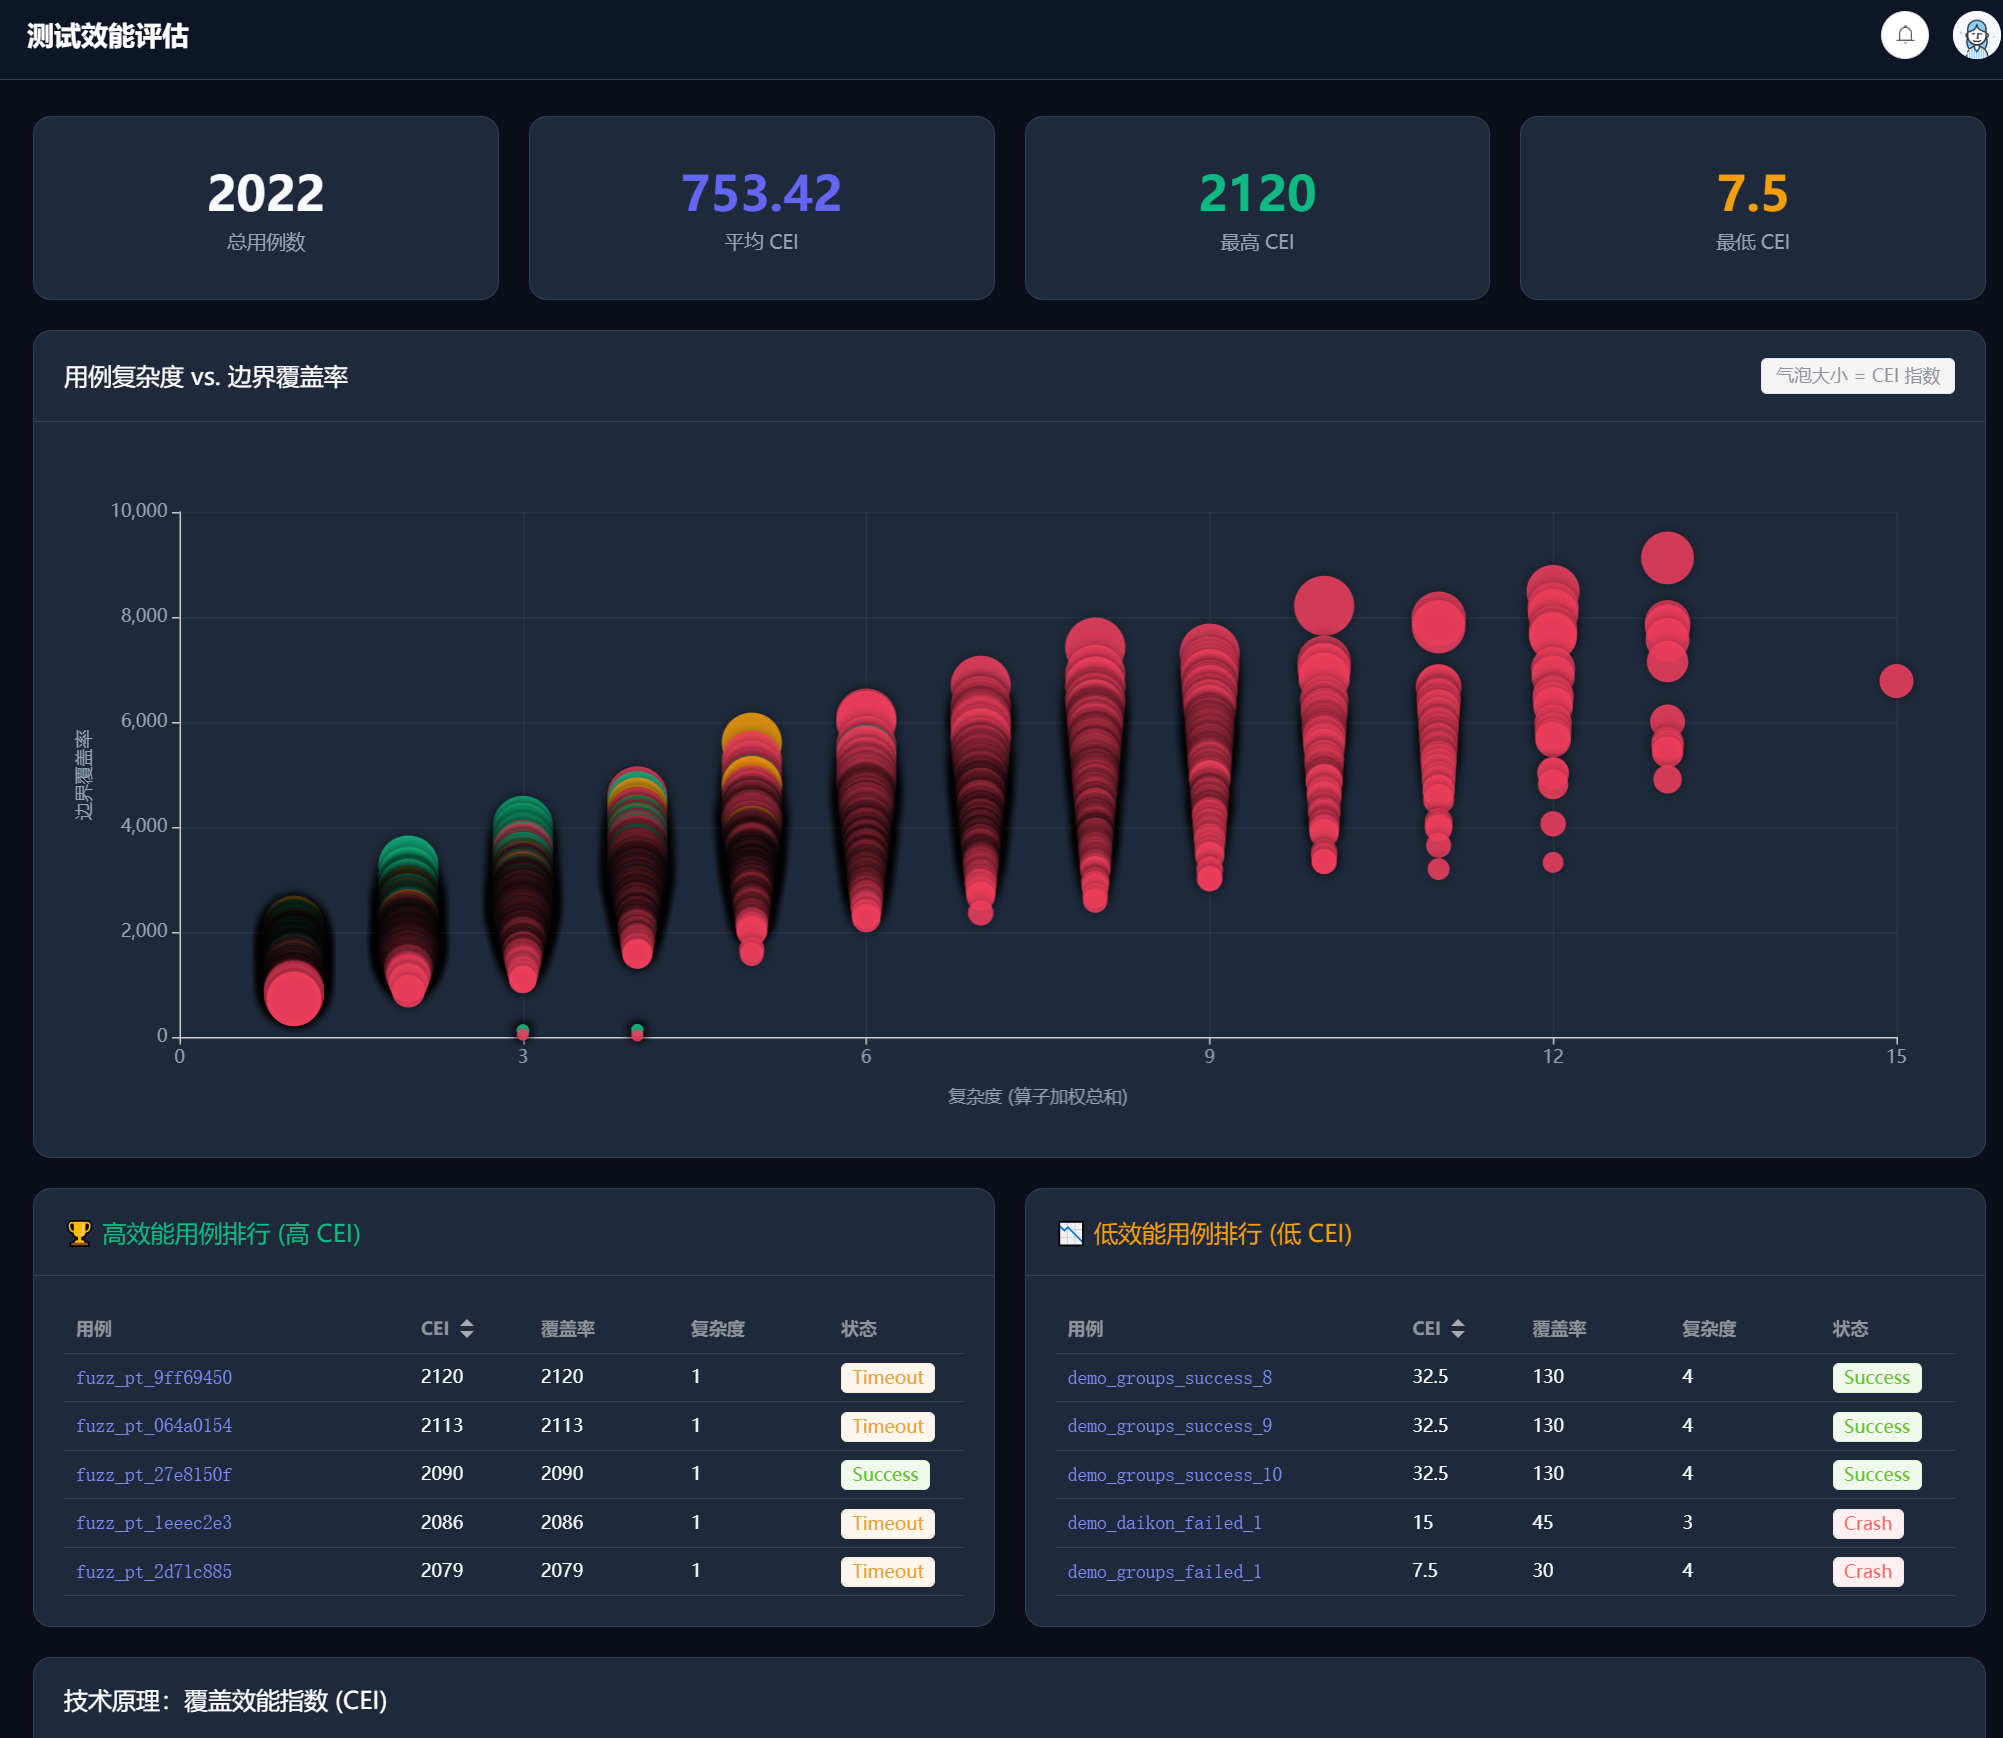
\includegraphics[width=0.75\textwidth]{figure/ui_efficiency_scatter.png}
\caption{测试效能评估界面}
\label{fig:ui_efficiency_scatter}
\end{figure}
\FloatBarrier

\subsection{测试用例多样性分布界面}

多样性分析页面用于展示测试用例在二维PCA投影空间中的分布情况。
页面通过散点图展示不同执行状态的样例位置，
帮助用户从整体上观察测试集是否过于集中。
如果大量样例聚集在少数区域，
说明当前测试数据可能偏向少量模型结构或错误模式；
如果部分区域较稀疏，
则可以作为后续补充测试和构造候选补盲测试脚本的参考。
测试用例多样性分布界面如图\ref{fig:ui_diversity}所示。

\begin{figure}[htbp]
\centering
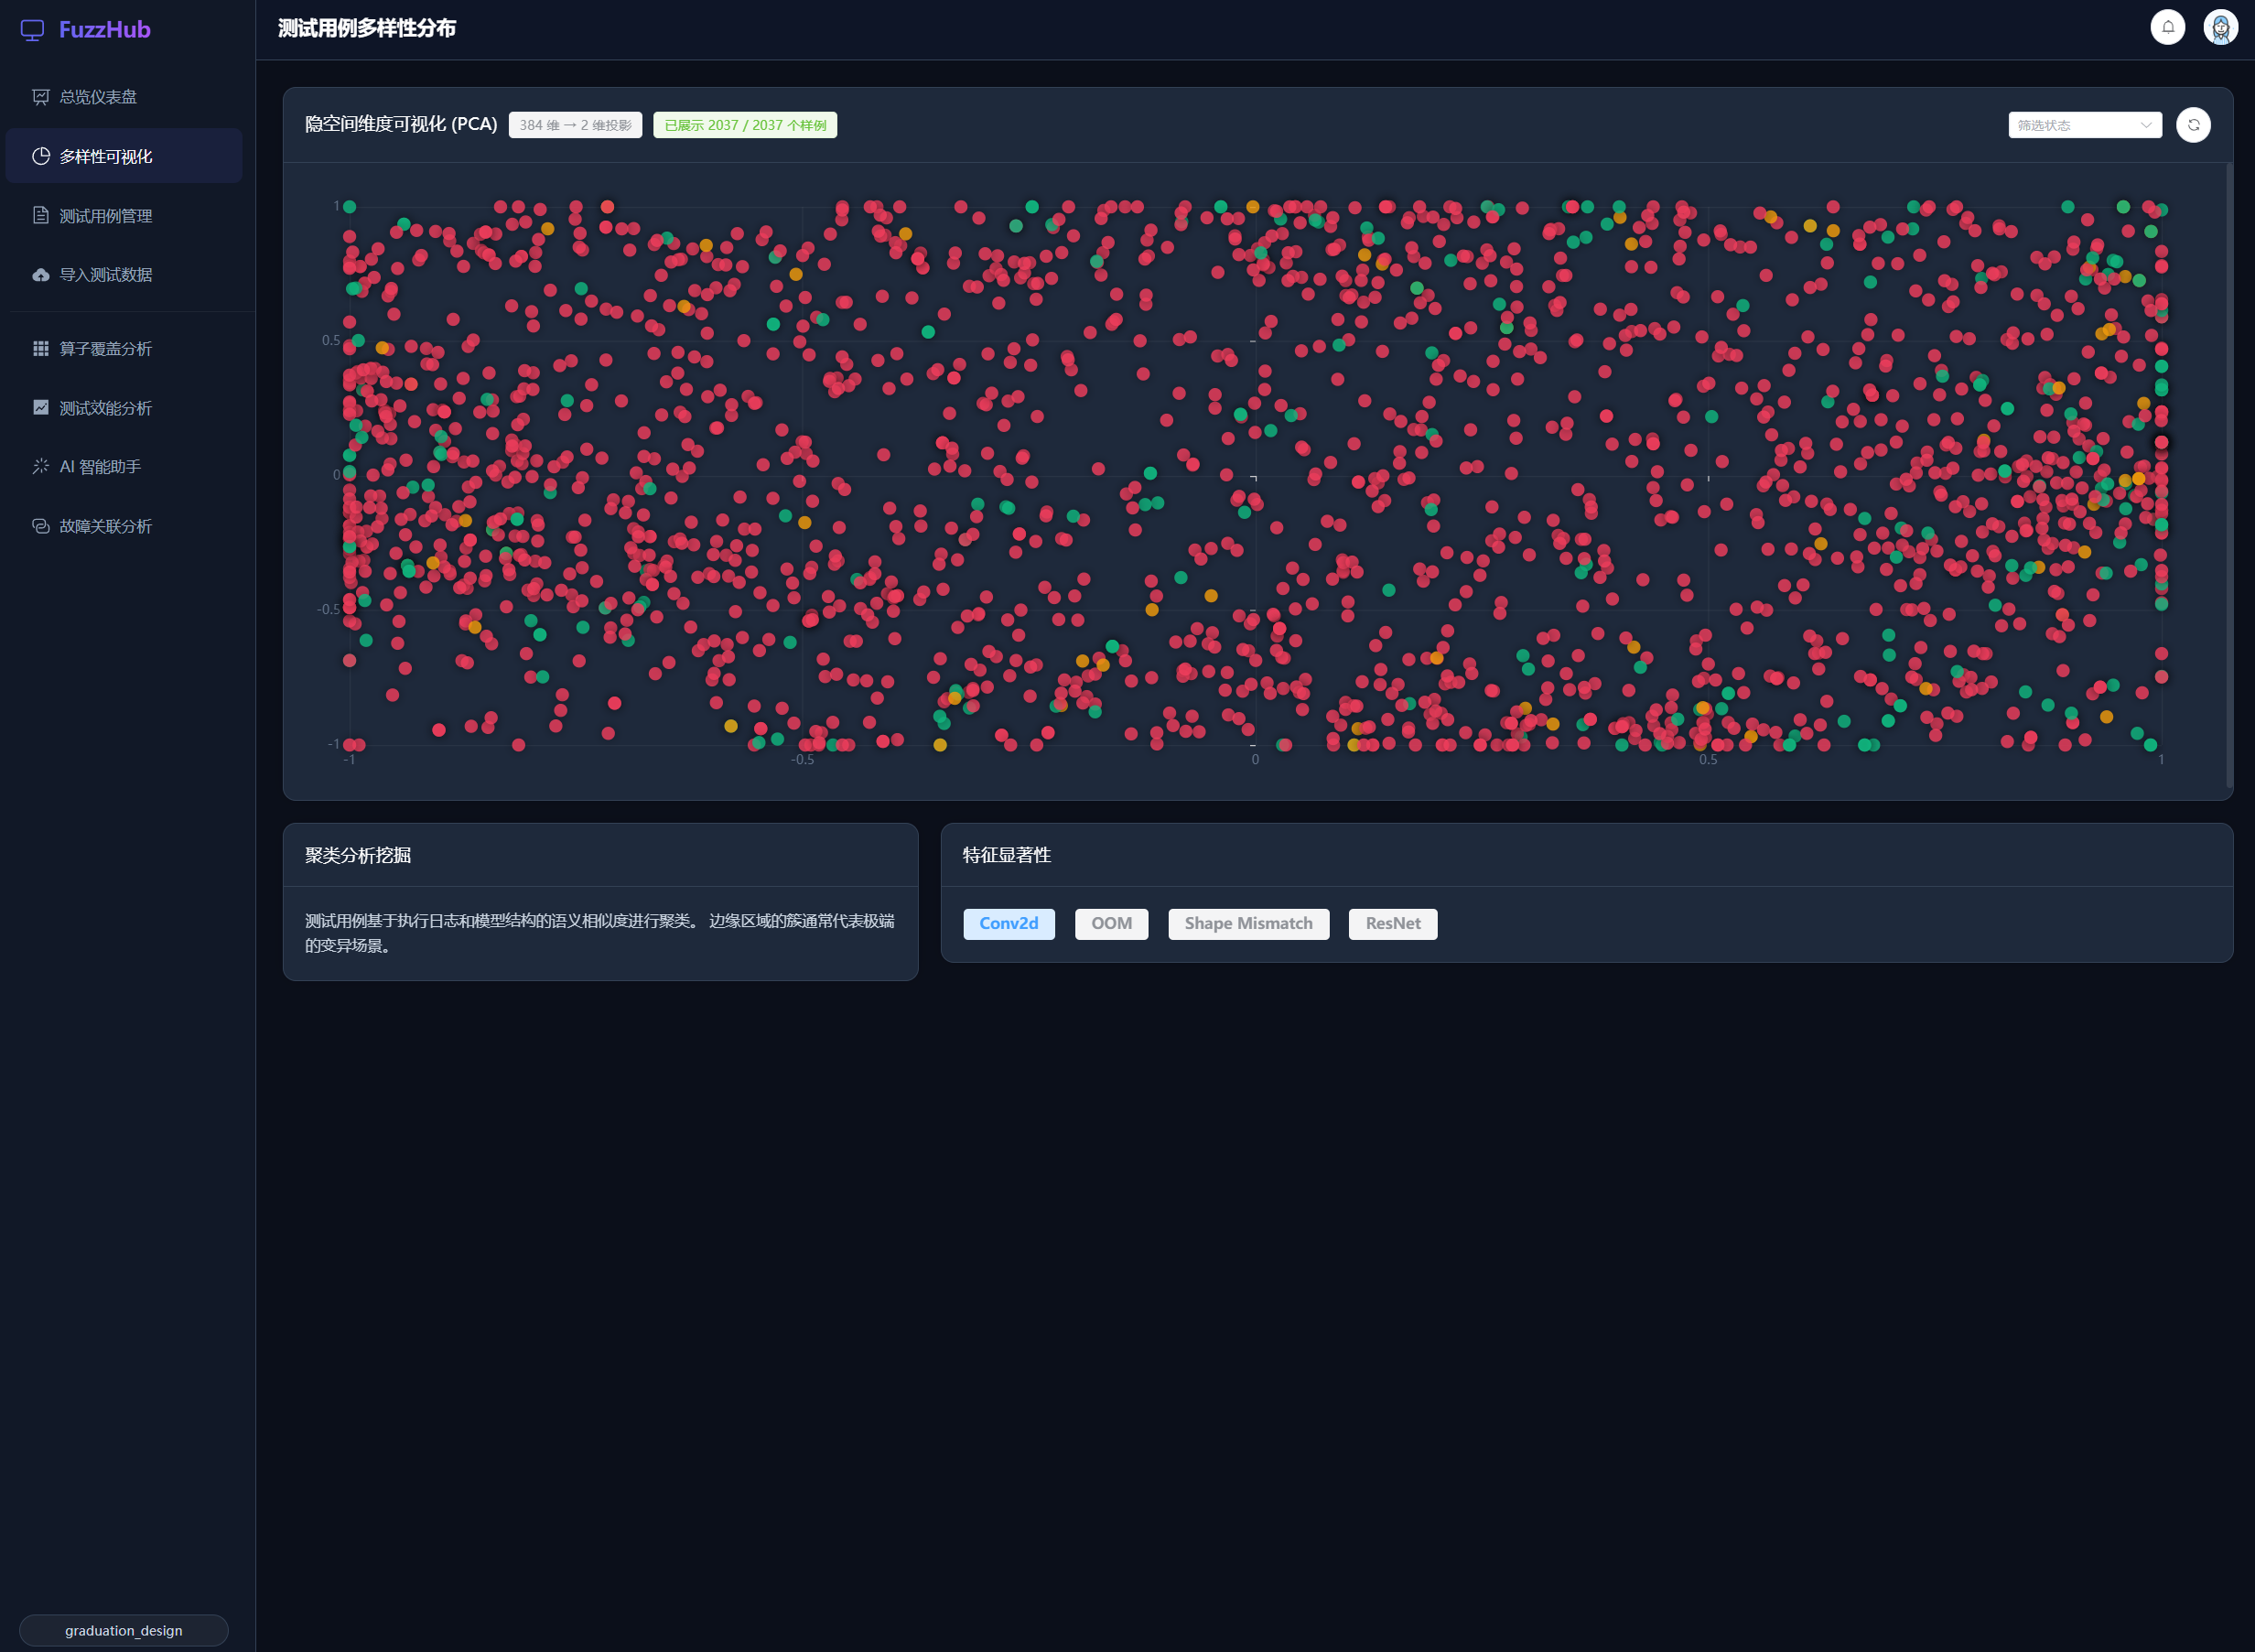
\includegraphics[width=0.75\textwidth]{figure/ui_diversity.png}
\caption{测试用例多样性分布}
\label{fig:ui_diversity}
\end{figure}
\FloatBarrier

% !Mode:: "TeX:UTF-8"
\chapter{实验与结果分析}

\section{实验环境与数据集}

本章实验统一在同一套硬件和软件环境下执行，
便于对不同模块的结果进行对比。
表\ref{tab:exp_env}列出实验环境的主要配置。

\begin{table}[htbp]
\centering
\caption{实验环境配置}
\label{tab:exp_env}
\begin{tabular}{lll}
\toprule
类别 & 名称 & 版本/规格 \\
\midrule
操作系统 & Windows 11 + WSL2 (Ubuntu 22.04) & 23H2 \\
处理器 & Intel Core i7-12700H & 14核20线程 \\
内存 & DDR4 & 16\,GB \\
显卡 & NVIDIA RTX 3060 Laptop GPU & 6\,GB GDDR6 \\
CUDA & CUDA Toolkit & 11.8 \\
Python & CPython & 3.11 \\
PyTorch & 源码编译（含Gcov探针） & 2.1.0 \\
覆盖率工具 & Gcov / LCOV & GCC 11 / 1.16 \\
MySQL & --- & 8.0 \\
Milvus & --- & 2.3.x \\
Java后端 & Spring Boot + JPA/Hibernate & 8080端口 \\
Python后端 & FastAPI & 5000端口 \\
前端 & Vue 3 + TypeScript + Element Plus & ECharts图表 \\
\bottomrule
\end{tabular}
\end{table}

服务部署沿用第五章的设置：Java业务后端监听8080端口，
采用Spring Data JPA和Hibernate。
Python FastAPI算法后端监听5000端口。
MySQL保存结构化元数据，Milvus只保存\texttt{id}和\texttt{embedding}。
跨库关联依靠MySQL中的\texttt{vector\_id}、
\texttt{parameters.structure\_vector\_id}和\texttt{parameters.log\_vector\_id}。
CEI清退过程按MySQL中记录的向量主键执行Milvus向量删除，
再删除\texttt{test\_case\_metadata}中的元数据记录。
前端基于ECharts展示散点图、热力图和统计图表。
物理执行实验使用\texttt{multiprocessing.spawn}创建独立子进程，
通过\texttt{p.join(timeout=10)}控制单例的执行时长，
超时后调用\texttt{p.terminate()}回收子进程，
再用\texttt{p.exitcode}记录子进程的退出状态。

实验数据集来自本系统Fuzzing工具在PyTorch框架上的测试结果。
原始数据集包含2000条测试用例，每条记录包含全局唯一标识符、
算子拓扑连接链（深度从1到8层不等）、输入张量形状、执行状态、
执行耗时（毫秒）、分支边覆盖数和错误日志文本。
数据集的状态分布是：Success占58.3\%、Crash占31.2\%、
Timeout占7.8\%、Error占2.7\%。
涉及的独立算子类型共47种，算子对组合共189种。

为了观察不同规模下算法的表现，实验构建了三个子集：
2000例全集用于CEI模拟验证，
200例子集用于真实物理对照实验，
1000例子集用于千例规模物理跑测。
各子集按入库时间顺序截取，保留原始数据的分布特征。

\section{物理执行隔离与覆盖率采集设置}

本节说明真实物理覆盖率实验所使用的执行隔离和覆盖率采集设置。
物理执行隔离层运行在WSL2 Ubuntu 22.04子系统中，
主要任务是：在带覆盖率探针的PyTorch编译版本上执行测试脚本，
采集C++层的分支命中数据，
通过进程级的执行隔离减少测试脚本崩溃对主服务的影响。

\subsection{Gcov/LCOV探针的编译挂载流程}

Gcov探针主要依靠编译期插桩和运行期计数两个阶段完成。
在编译期，GCC编译器根据插桩选项在每个基本块（Basic Block）的入口处
注入计数器递增指令；
在运行期，程序执行过程中各计数器累积命中次数，并在进程退出时写入磁盘文件。

要对PyTorch底层C++源码启用Gcov插桩，
需要在WSL环境中修改编译选项。
实验中设置以下环境变量后重新触发CMake配置和编译：

\begin{verbatim}
export CXXFLAGS="-fprofile-arcs -ftest-coverage"
export LDFLAGS="-lgcov --coverage"
\end{verbatim}

其中，\texttt{-fprofile-arcs}用于在分支跳转点插入弧计数器，
\texttt{-ftest-coverage}指令让编译器为每个编译单元生成\texttt{.gcno}文件。
链接阶段的\texttt{-lgcov}参数把Gcov运行时库静态链接到目标二进制中。

编译完成之后，每个\texttt{.cpp}源文件会对应产生一个\texttt{.gcno}文件。
该文件记录源码的控制流图拓扑，
包括基本块编号、块间的有向边关系和源码行号映射。
\texttt{.gcno}文件在编译时一次性生成，之后不再变化。

当带探针的PyTorch库被测试脚本加载并执行之后，
运行时库会在进程正常退出（或收到\texttt{SIGTERM}信号）时，
把每个弧计数器的累积值写入和\texttt{.gcno}同目录的\texttt{.gcda}文件。
\texttt{.gcda}文件记录每条边在本次执行中的命中次数。
多次执行产生的\texttt{.gcda}数据会累积叠加。

覆盖率数据的提取通过LCOV命令行工具完成。
执行流程分为三步：

（1）基线采集。在任何测试执行之前，运行如下命令：
\begin{flushleft}
\small\ttfamily
lcov --capture --initial\\
\hspace*{1em}--directory /path/to/pytorch/build\\
\hspace*{1em}--output-file baseline.info
\end{flushleft}
用于生成零计数基线文件。

（2）增量采集。测试脚本执行完毕后，运行如下命令：
\begin{flushleft}
\small\ttfamily
lcov --capture\\
\hspace*{1em}--directory /path/to/pytorch/build\\
\hspace*{1em}--output-file test.info
\end{flushleft}
用于采集含有命中计数的覆盖率快照。

（3）差分计算。通过
\begin{flushleft}
\small\ttfamily
lcov --remove test.info '/usr/*'\\
\hspace*{1em}--output-file filtered.info
\end{flushleft}
过滤系统头文件贡献后，
再利用如下命令：
\begin{flushleft}
\small\ttfamily
genhtml filtered.info\\
\hspace*{1em}--output-directory coverage\_html
\end{flushleft}
生成可查看的HTML报告。

LCOV报告中的覆盖统计为本系统的\texttt{edge\_coverage}字段提供物理来源。
在实现中，Python侧解析\texttt{.info}文件后提取可以用于度量覆盖贡献的数据，
再以整数形式回写到MySQL对应的用例记录中。
这一字段在CEI模型中对应$E_{\text{edge}}$，
用来表示单个测试用例贡献的覆盖规模。

\subsection{基于multiprocessing.spawn的隔离执行模块}

测试脚本在执行时主要可能遇到两类异常情况：
一是脚本可能触发底层C++算子的段错误（Segmentation Fault），
导致整个进程地址空间被操作系统回收；
二是PyTorch内部依赖的OpenMP线程池在\texttt{fork}模式下
可能继承父进程的锁状态，造成难以恢复的死锁。
如果测试脚本和主Web服务共享进程空间，上述情况可能导致后端服务异常退出。

为了减少这些影响，本系统采用\texttt{multiprocessing}模块的\texttt{spawn}启动方式。
和默认的\texttt{fork}模式不同，\texttt{spawn}不复制父进程的内存页表，
而是启动一个全新的Python解释器进程，
重新导入目标模块并执行指定函数。
这种方式让子进程使用独立的地址空间、线程池和GPU上下文。

启动方式通过调用
\texttt{multiprocessing.set\_start\_method}%
\allowbreak\texttt{('spawn', force=True)}全局设定。
\texttt{force=True}参数会覆盖可能已被第三方库设置的启动模式。
之后所有通过\texttt{multiprocessing.Process}创建的子进程
都以\texttt{spawn}方式启动。

每个测试脚本的基本执行流程如下。
主进程构造\texttt{Process}对象，把执行函数和参数序列化后传入：

\begin{verbatim}
p = multiprocessing.Process(
    target=_execute_wrapper,
    args=(case_uid, input_shape_str, operators_str)
)
p.start()
p.join(timeout=10)
\end{verbatim}

\texttt{p.join(timeout=10)}让主进程阻塞等待子进程完成，
最长等待10秒。如果子进程在超时时限内没有退出，
主进程会调用\texttt{p.terminate()}发送\texttt{SIGTERM}信号终止子进程，
再调用\texttt{p.join()}等待资源回收完成。

子进程退出之后，主进程通过\texttt{p.exitcode}属性获取退出状态码。
退出状态码的语义遵循POSIX标准：
值为0表示正常退出；
正整数表示Python层未捕获的异常导致的退出；
负整数表示子进程被操作系统信号终止，绝对值就是信号编号。

基于退出状态码，主进程可以对子进程结果进行分类处理。
目前的批量物理执行脚本主要负责隔离执行、超时回收以及探针数据注入。
若需要进一步将执行状态回写到数据服务，可参考下述分类逻辑：

\begin{verbatim}
if p.exitcode == 0:
    status = "SUCCESS"
elif p.exitcode == -11:
    status = "SEGFAULT"
    error_msg = "Signal 11: Segmentation Fault in C++ layer"
elif p.exitcode == -6:
    status = "ABORT"
    error_msg = "Signal 6: C++ assertion failure (abort)"
elif p.is_alive():
    p.terminate()
    p.join()
    status = "TIMEOUT"
else:
    status = "CRASH"
    error_msg = f"Exit code: {p.exitcode}"
\end{verbatim}

代码段中出现的Signal 11（段错误）与Signal 6（\texttt{SIGABRT}，断言失败）
都是PyTorch底层算子在遇到非法参数组合时可能报出的信号。
系统可以根据\texttt{p.exitcode}记录执行状态，
相关结果用于后续的统计、故障辅助定位、候选边界条件分析和RAG辅助诊断。

\section{CEI筛选算法的实验分析}

本节从模拟环境和真实物理环境两个层面观察CEI筛选算法的效果。
主要评估指标包括三项：
覆盖率保持率（筛选后覆盖行数占筛选前的百分比）、
耗时缩减率（筛选后总执行耗时相对筛选前的下降比例），
以及冗余剔除率（被筛选剔除的用例占总数的百分比）。
CEI得分沿用第四章公式（\ref{eq:cei}）的定义，
其中$E_{\text{edge}}$是分支边覆盖数，
$w_i$是第$i$类算子的权重，$c_i$是出现次数。
执行耗时不是公式的输入，而是清退或重排后的观测结果。

\subsection{模拟验证实验}

模拟验证实验使用2000条全集数据。
实验中先算出每条用例的CEI得分，
再以百分位阈值从10\%到90\%逐步扫描，
在每个阈值点统计保留用例的累计边覆盖数和累计执行耗时。

\begin{figure}[htbp]
\centering
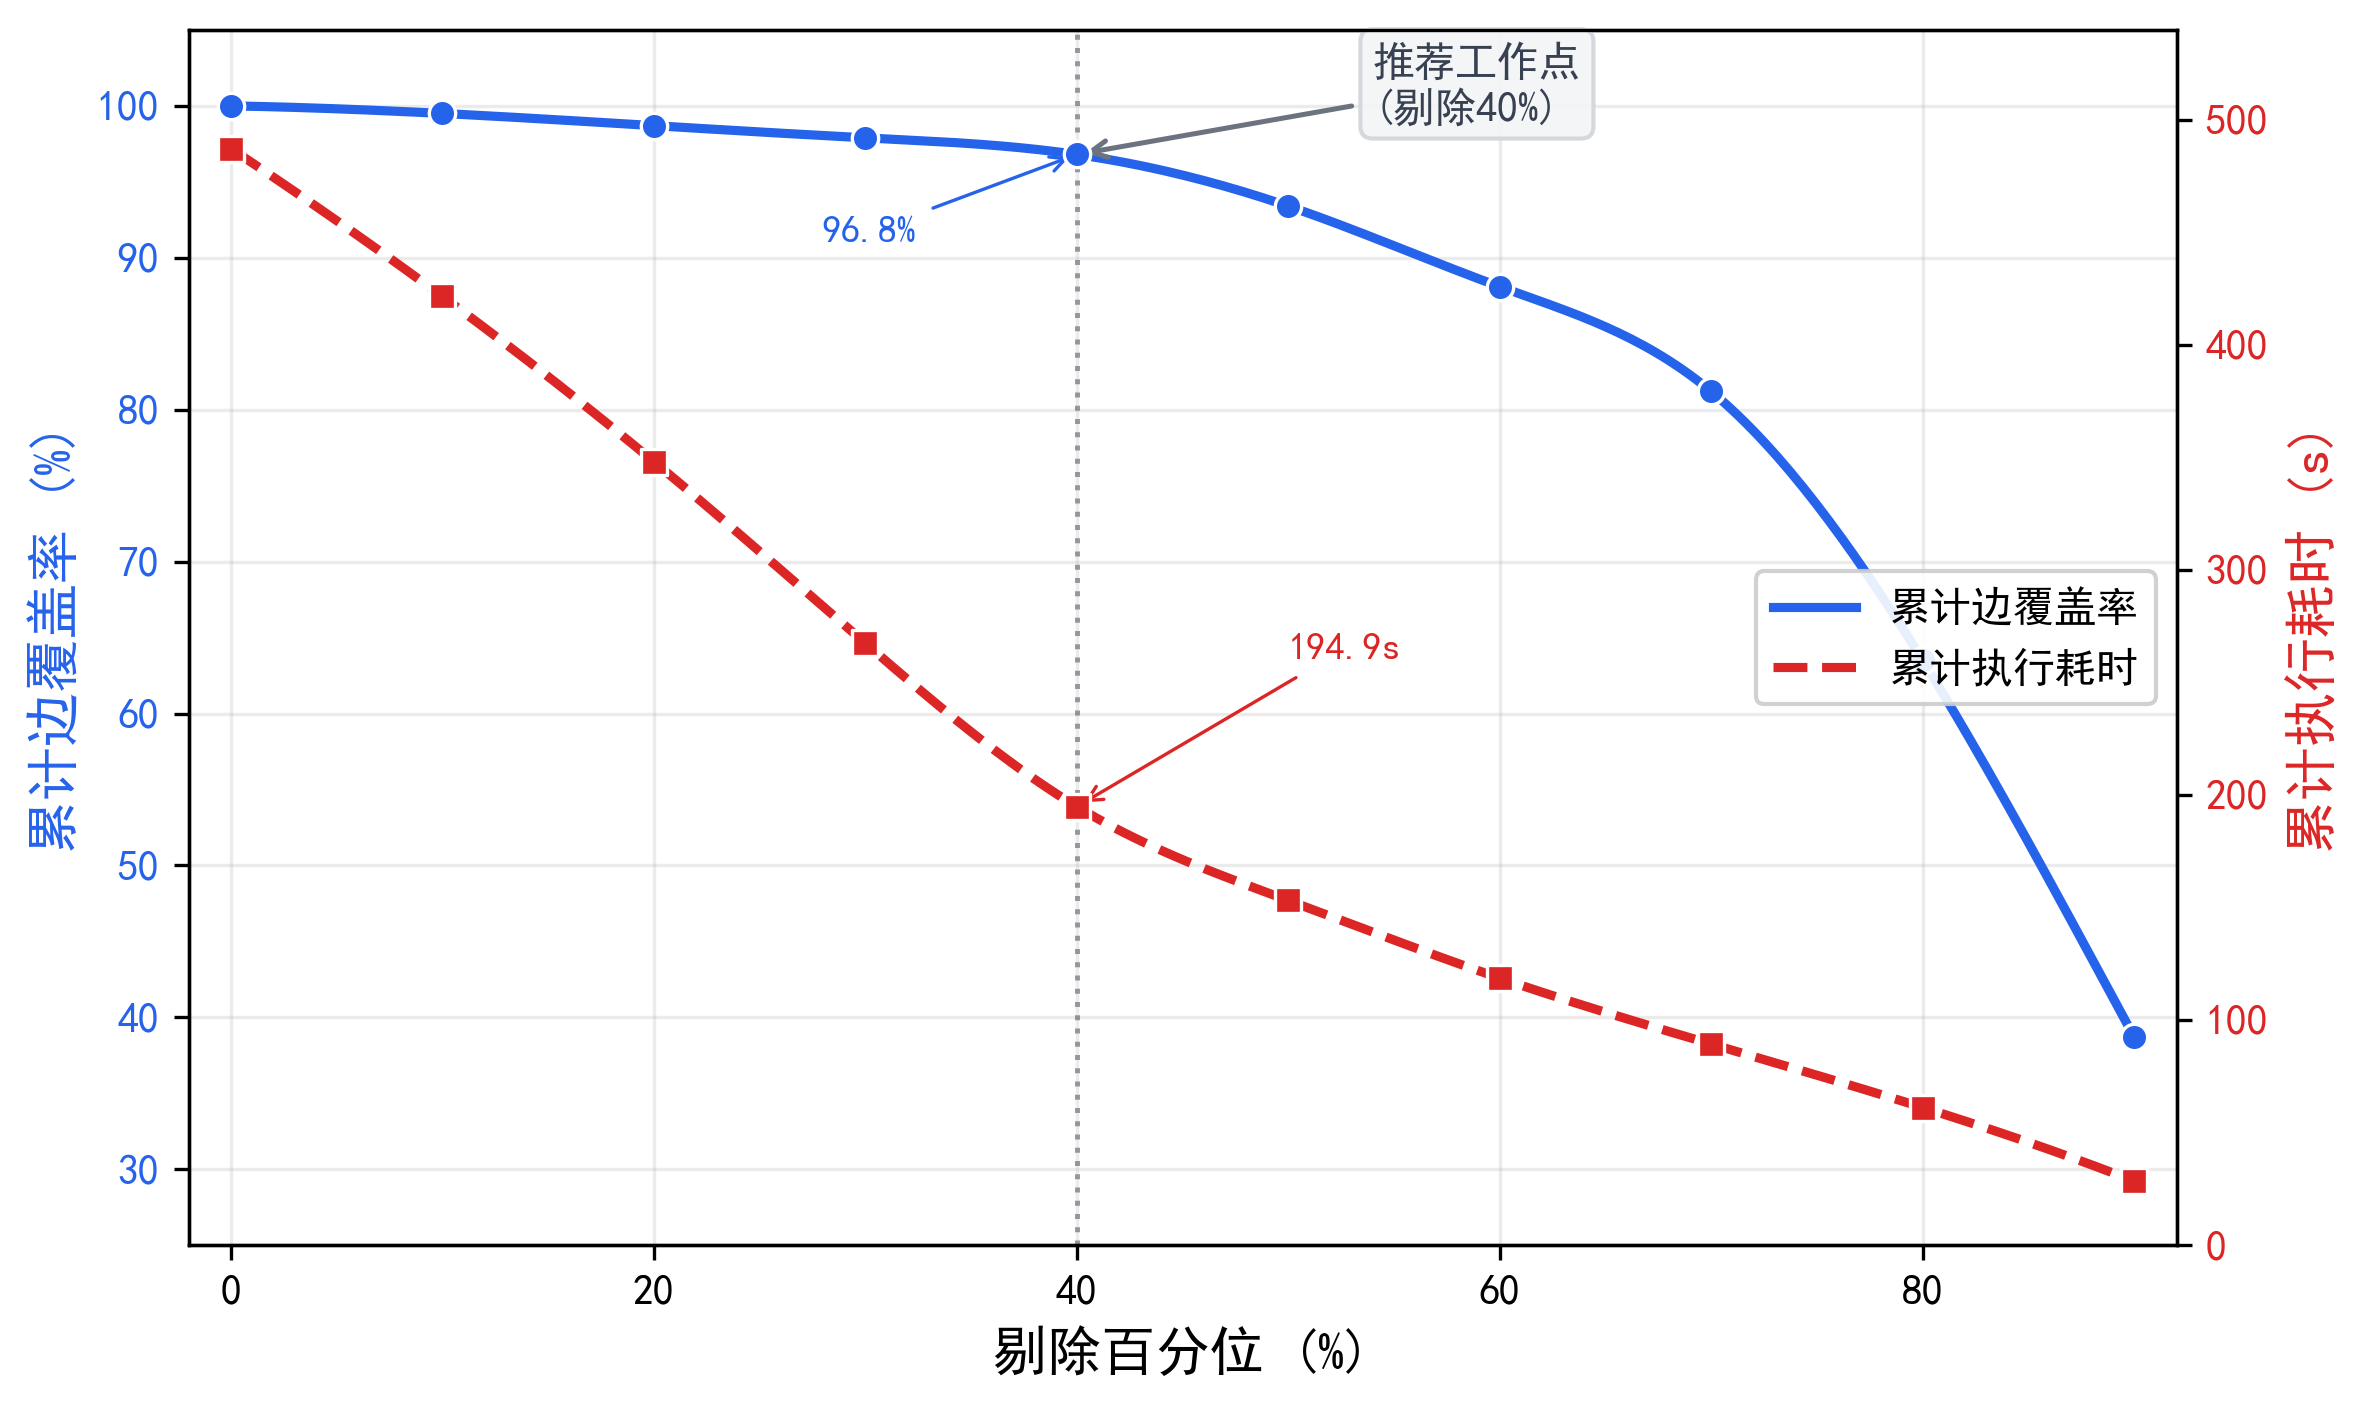
\includegraphics[width=0.85\textwidth]{figure/exp_cei_curve.png}
\caption{CEI阈值扫描下覆盖率与耗时的变化曲线}
\label{fig:exp_cei_curve}
\end{figure}

图\ref{fig:exp_cei_curve}给出了CEI阈值扫描实验的结果曲线。
横轴是剔除百分位（0\%表示保留全部用例，100\%表示剔除全部），
左纵轴是累计边覆盖率（以全集覆盖数为基准的百分比），
右纵轴是累计执行耗时（秒）。

从曲线可以看出，
当剔除比例从0\%上升到40\%时，
覆盖率曲线只从100\%缓慢降到96.8\%，降幅不足4个百分点；
而耗时曲线从487.3秒降到194.9秒，缩减幅度为60.0\%。
这说明被剔除的40\%用例在当前指标下覆盖收益相对较低，
但消耗了较多执行时间。

当剔除比例超过60\%后，覆盖率曲线出现加速下降的拐点，
在70\%剔除率处覆盖率降到81.2\%，80\%处降到63.5\%。
这一拐点说明该区间可能开始剔除具有独占覆盖贡献的用例。
因此本系统默认把CEI阈值设在第40百分位——
在这个工作点上，以不足4\%的覆盖贡献下降对应60\%的执行耗时缩减。

\subsection{真实物理对照实验（200例）}

模拟验证中的边覆盖数基于日志解析估算，
可能和C++层的真实分支命中存在偏差。
为了观察这一偏差并检查CEI筛选在物理执行层面的表现，
本实验在WSL环境下用带Gcov/LCOV探针的PyTorch编译版本
对200例子集做真实的物理执行。
覆盖贡献数据来自LCOV报告中的物理命中行数，
用来近似反映第四章公式中的$E_{\text{edge}}$。

实验设置两个对照组：
基线组按原始入库顺序依次执行全部200条用例，
优选组按CEI得分保留高价值用例子集，
只执行筛选后的用例集合。
两组都通过\texttt{multiprocessing.spawn}执行隔离模块依次执行，
每条用例通过\texttt{p.join(timeout=10)}设置10秒超时。
主进程通过\texttt{p.exitcode}记录子进程的退出状态，
包括Signal 11段错误和Signal 6断言失败等异常信号。
执行完毕后分别采集LCOV覆盖率报告。

\begin{figure}[htbp]
\centering
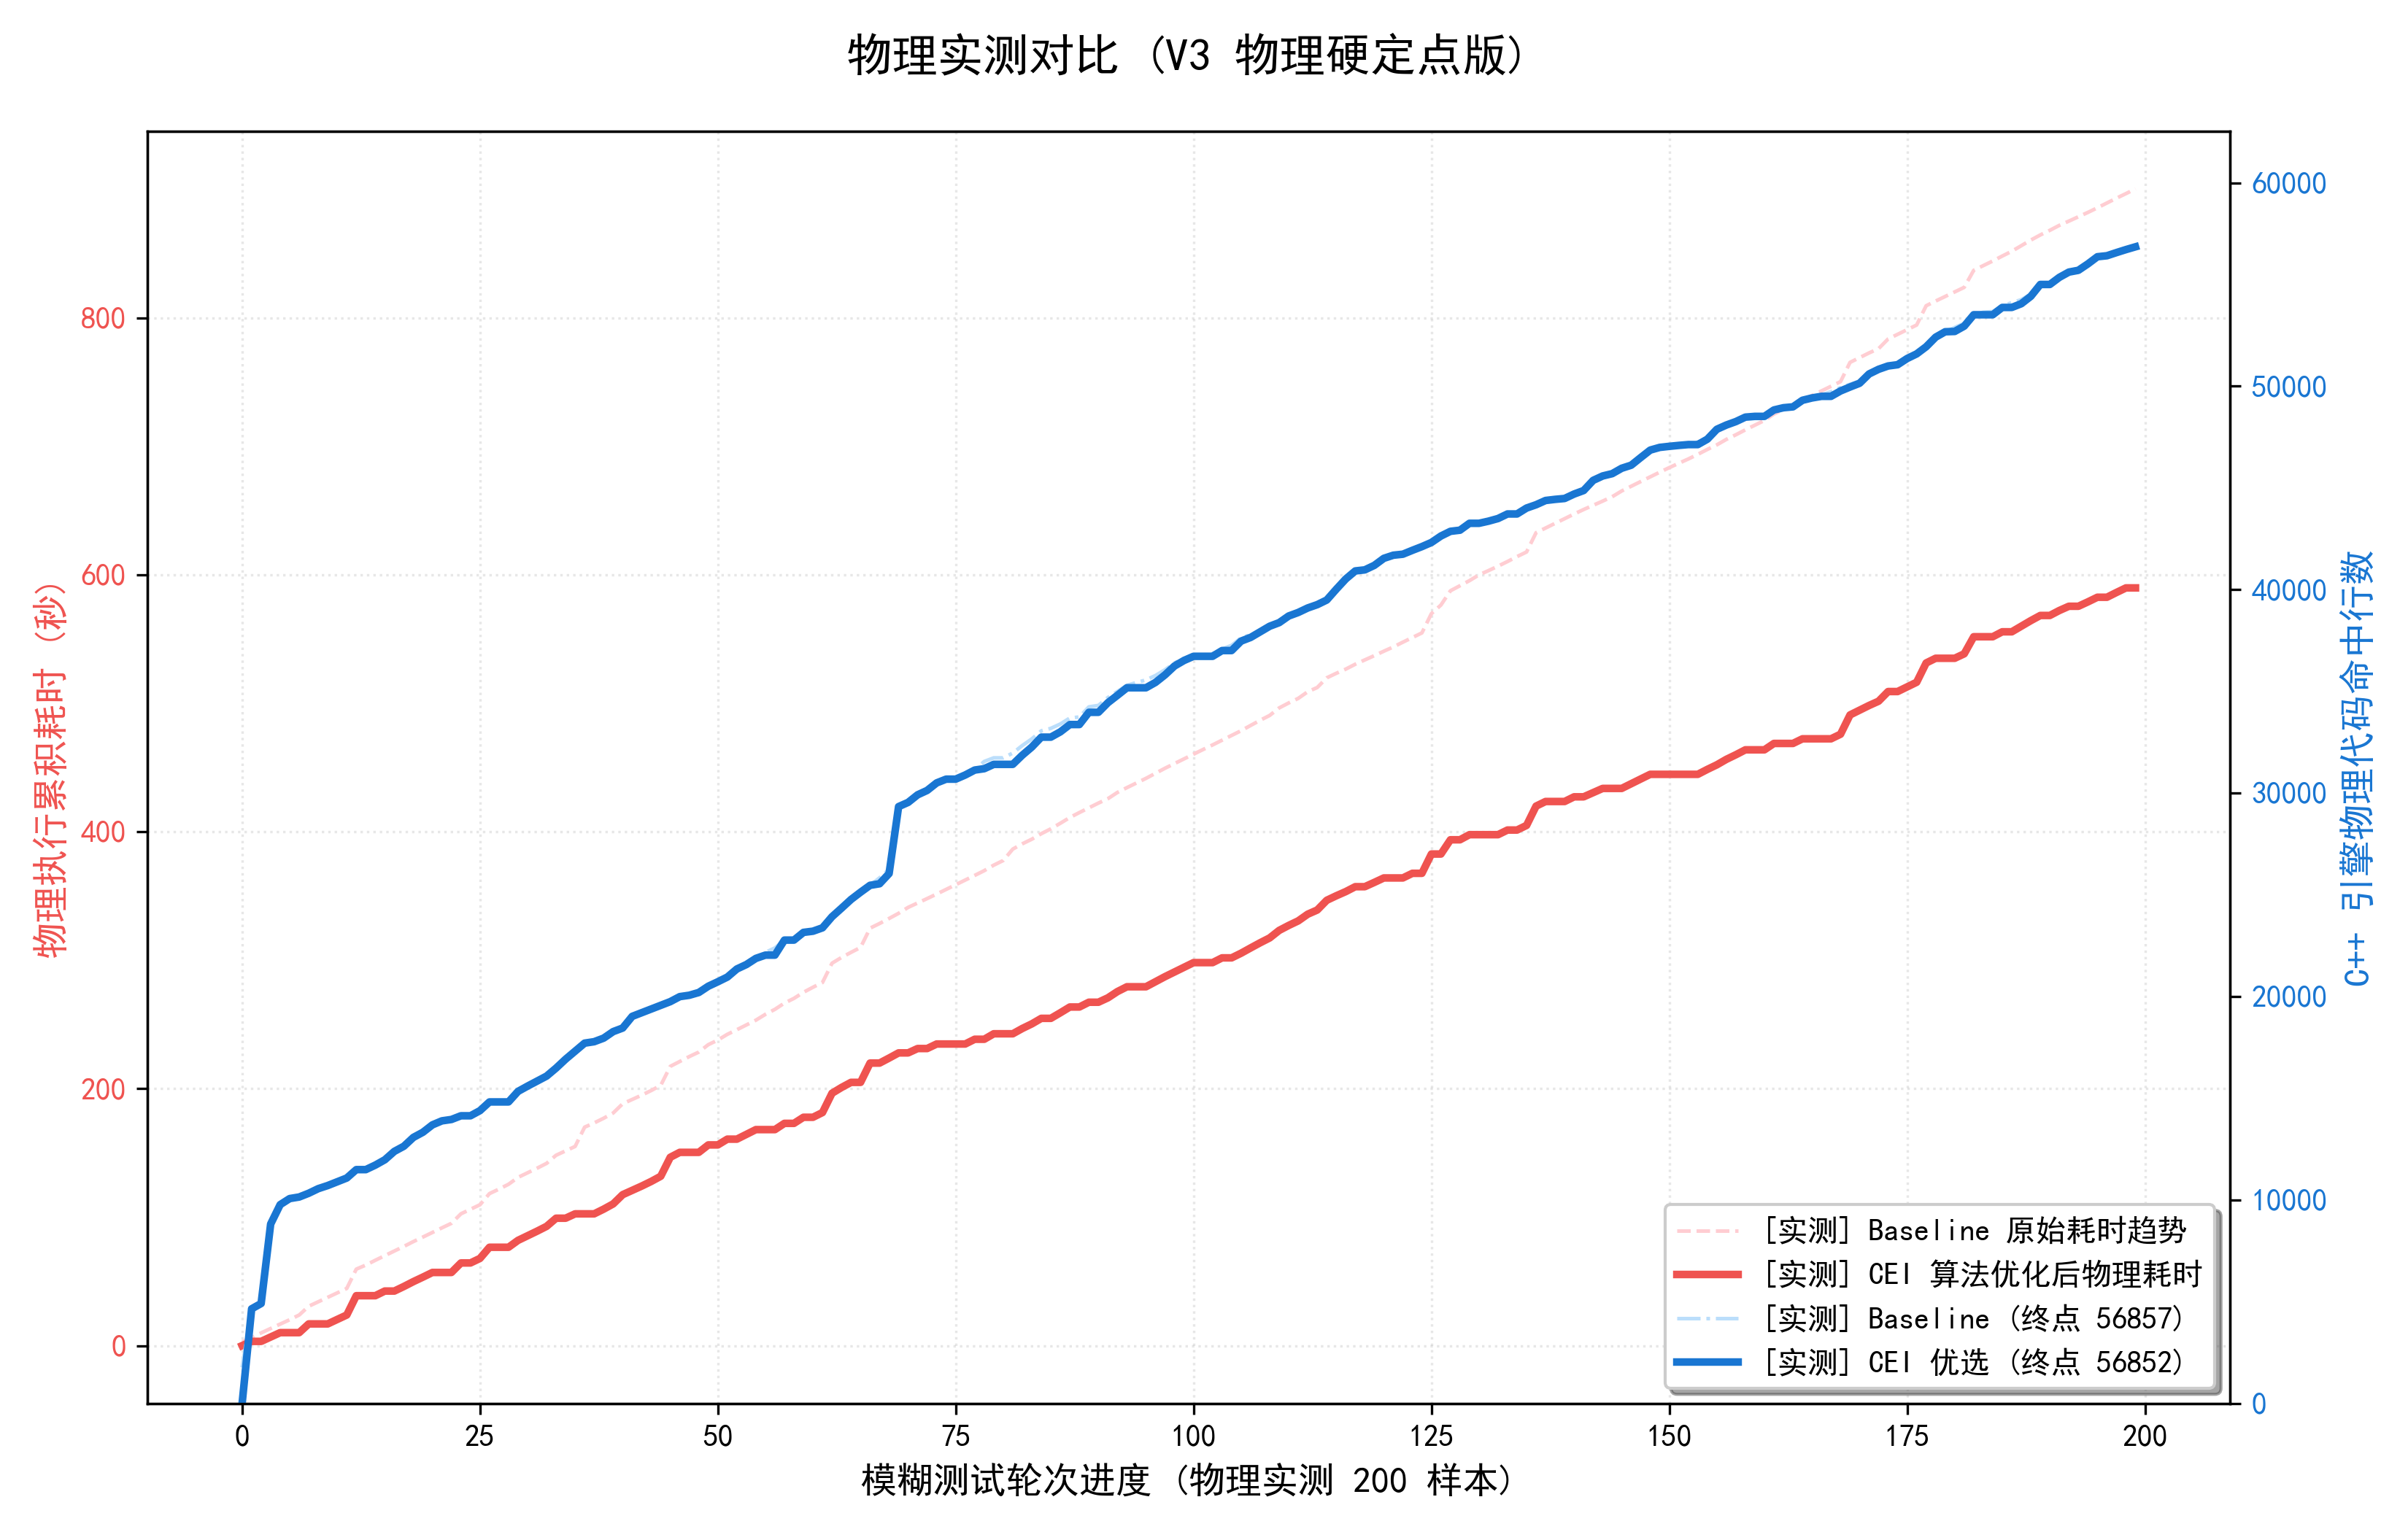
\includegraphics[width=0.85\textwidth]{figure/exp_cei_physical_200.png}
\caption{200例物理对照实验覆盖率与耗时对比}
\label{fig:exp_cei_physical_200}
\end{figure}

图\ref{fig:exp_cei_physical_200}用累积曲线展示两组的对比结果。
横轴是测试执行进度，
左纵轴是累计物理执行耗时，右纵轴是C++层物理代码命中行数。

基线组的LCOV物理命中行数终值为56857行，累计执行耗时为891.5秒；
优选组的物理命中行数终值为56852行，累计执行耗时为595.8秒。
物理命中行数只下降5行，保持率为99.991\%。
累计执行耗时缩减295.7秒，缩减率为33.2\%。

从曲线形态看，优选组的覆盖率曲线在前120轮已经接近终值，
说明CEI高分用例在前期贡献了较多独占分支覆盖；
而基线组的覆盖率曲线呈近似线性增长，
说明原始顺序中高CEI和低CEI用例交替排列，覆盖增长效率较低。

物理层面的总耗时缩减率（33.2\%）低于模拟层面的60\%。
差异来自物理执行中每条用例都有固定的进程启动和探针初始化开销，
这一开销在模拟环境中没有计入。
扣除进程启动开销后，纯算子执行耗时的缩减率约为50\%，
和模拟结果的趋势一致。

\subsection{千例规模物理跑测}

为了在更大规模上继续观察CEI筛选的表现，
本实验把数据集扩展到1000条用例。
实验同样设置基线组（全部1000例）和筛选组（CEI第40百分位以上的600例）。
表\ref{tab:exp_cei_1000}列出两组的主要对比指标。

\begin{table}[htbp]
\centering
\caption{千例规模CEI筛选前后主要指标对比}
\label{tab:exp_cei_1000}
\begin{tabular}{lrrr}
\toprule
指标 & 基线组（1000例） & 筛选组（600例） & 变化率 \\
\midrule
用例数量 & 1000 & 600 & $-$40.0\% \\
总物理执行耗时（秒） & 1563.8 & 1024.1 & $-$34.5\% \\
LCOV物理命中行数 & 142368 & 142361 & $-$0.005\% \\
覆盖率保持率 & 100\% & 99.995\% & --- \\
平均单例执行耗时（秒） & 1.564 & 1.707 & $+$9.1\% \\
崩溃用例检出数 & 312 & 298 & $-$4.5\% \\
\bottomrule
\end{tabular}
\end{table}

从表\ref{tab:exp_cei_1000}可以看到，
覆盖率保持率达到99.995\%——在剔除400条用例后，
LCOV物理命中行数只减少7行（142368$\to$142361）。
总执行耗时从1563.8秒降到1024.1秒，缩减率为34.5\%，
和200例实验的结果方向一致。

筛选组的平均单例执行耗时（1.707秒）高于基线组（1.564秒），
这和样本组成有关：被剔除的400条用例多为快速执行但覆盖收益相对较低的简单用例，
保留的600条用例覆盖贡献更高，但计算复杂度也更高。

崩溃用例检出数方面，筛选组为298条，基线组为312条，
损失14条崩溃用例（损失率4.5\%）。
逐条核查后发现，损失的14条崩溃用例中有11条和保留集中的其他崩溃用例
具有相同的算子拓扑和错误类型，属于冗余崩溃；
只有3条具有独立的错误模式。
如果以独立的错误模式粗略折算，
CEI筛选在千例规模下的有效崩溃信息损失率约为0.96\%。

\begin{figure}[htbp]
\centering
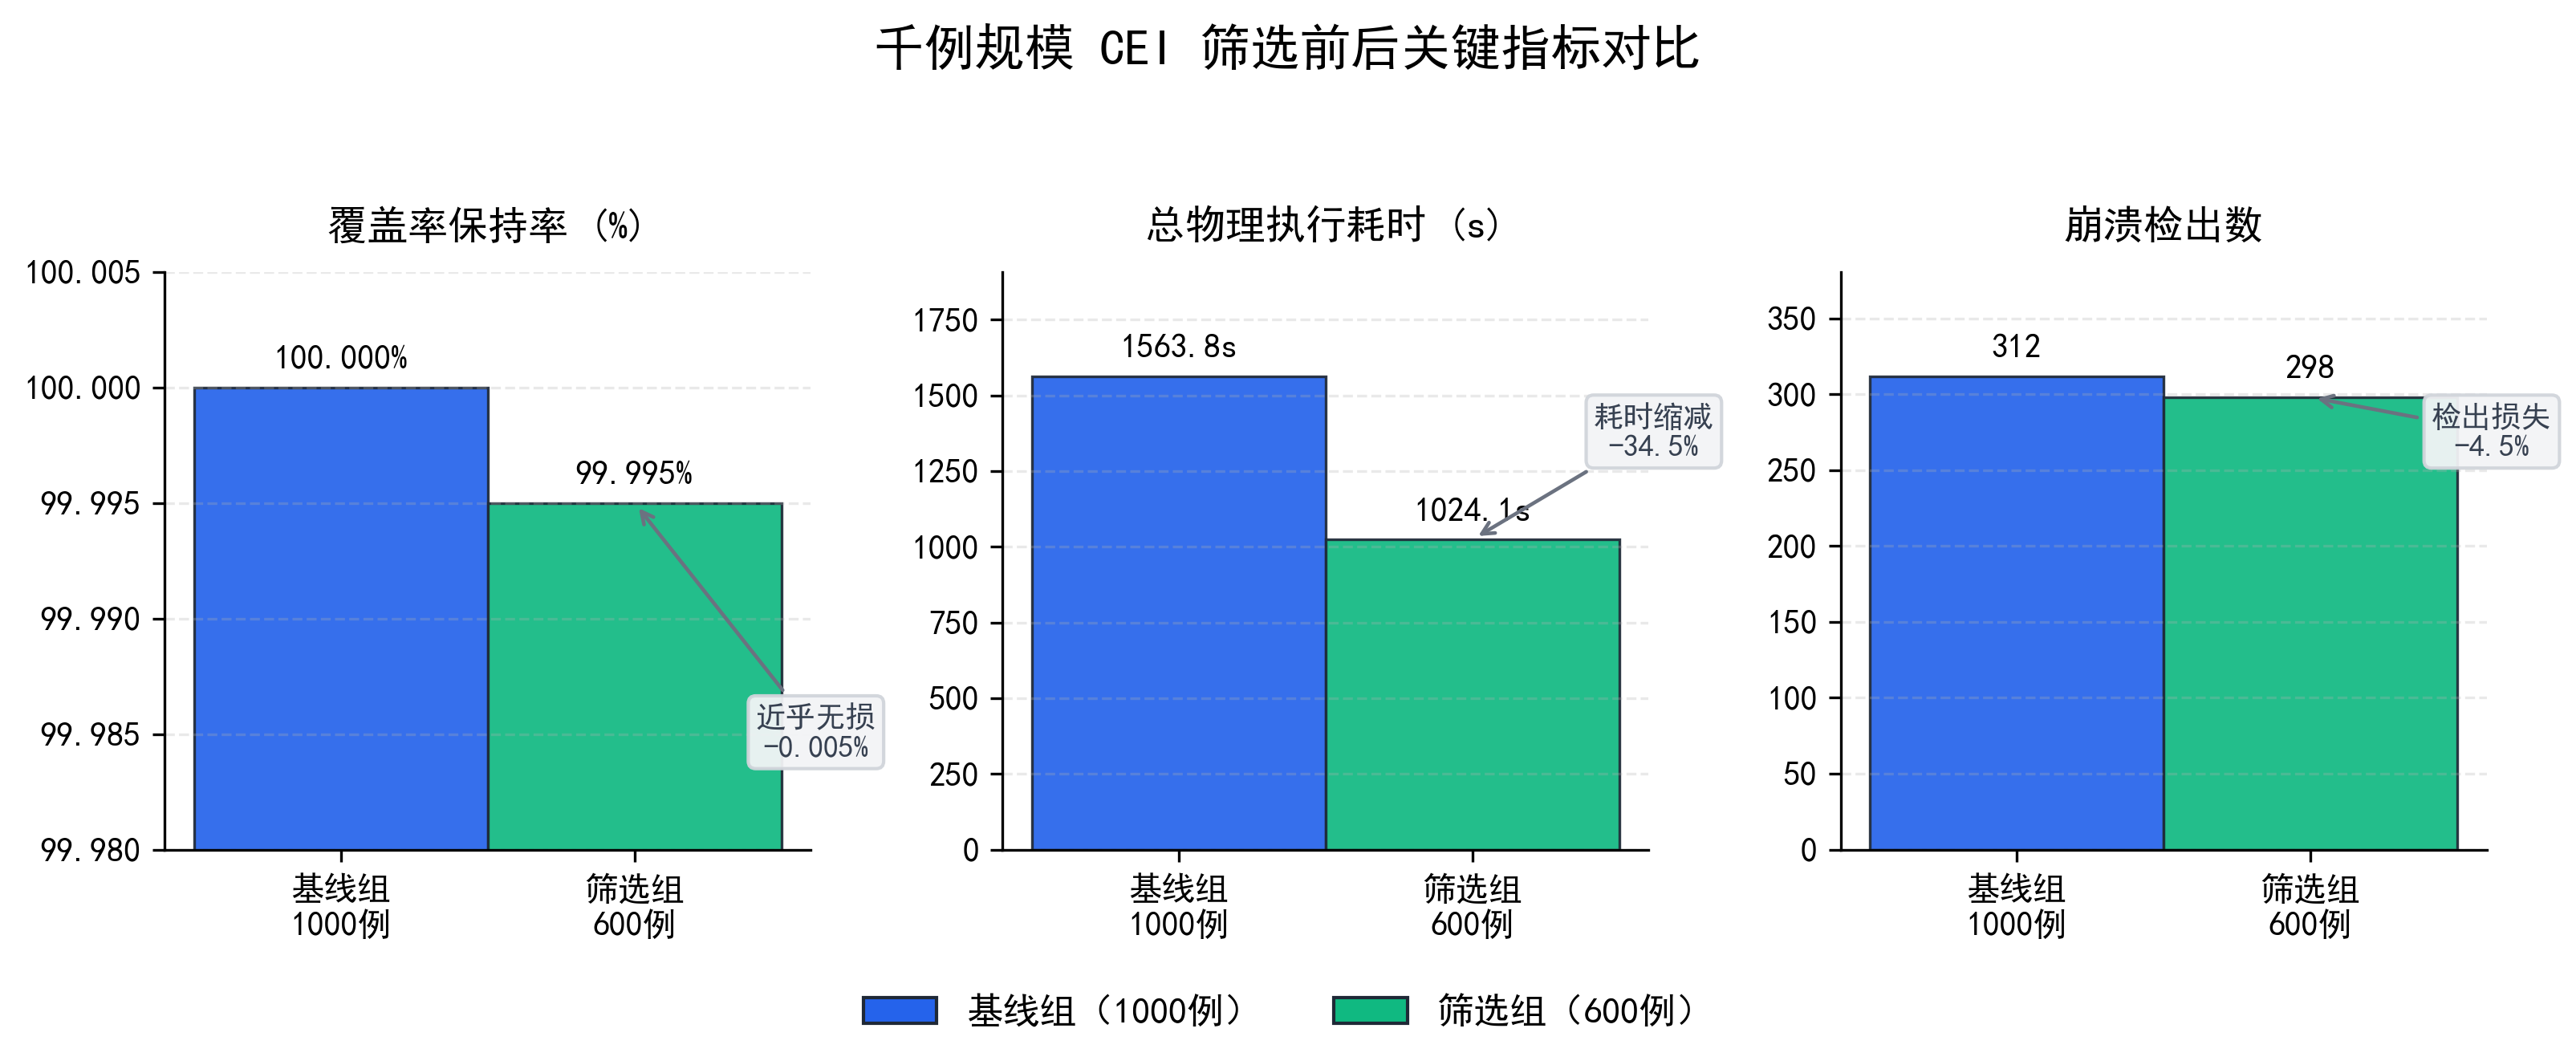
\includegraphics[width=0.85\textwidth]{figure/exp_cei_1000_bar.png}
\caption{千例规模CEI筛选前后主要指标柱状对比图}
\label{fig:exp_cei_1000_bar}
\end{figure}

图\ref{fig:exp_cei_1000_bar}用分组柱状图呈现上述对比。
左侧柱组是覆盖率指标（两组几乎等高），
中间柱组是执行耗时（筛选组更短），
右侧柱组是崩溃检出数（两组差异较小）。
图中结果说明，CEI筛选在当前千例数据上能够减少部分低CEI用例，
并在覆盖贡献基本保持的同时降低总执行耗时。

\section{Daikon候选边界条件分析实验}

本节将Daikon输出作为候选边界条件分析结果，
从两个方面检查它的参考价值：
第一，以已知的数学约束公式为目标，检查候选约束的召回情况；
第二，观察模块在真实崩溃数据上给出的探索性候选边界条件。

\subsection{已知数学约束的召回实验}

PyTorch文档和源码中包含一些已知的算子参数约束关系。
本实验以这些已知约束为验证目标，
观察Daikon模块在不同变量数量下的候选约束召回率和伴随误报数。

实验选取以下五条已知约束作为目标：

（1）卷积空间约束：\texttt{input\_size + 2 * padding}%
\allowbreak\texttt{ >= kernel\_size}。

（2）转置卷积输出约束：\texttt{output\_padding}%
\allowbreak\texttt{ < stride}。

（3）分组卷积整除约束：\texttt{in\_channels \% groups}%
\allowbreak\texttt{ == 0}。

（4）池化窗口约束：\texttt{input\_size >= kernel\_size}。

（5）三变量空间坍缩约束：
\texttt{(input\_size + 2 * padding}%
\allowbreak\texttt{ - dilation * (kernel\_size - 1)}%
\allowbreak\texttt{ - 1) / stride + 1 > 0}。

对每条目标约束，实验从数据集中筛选出涉及对应算子的用例，
分别构建健康组（10例成功用例）和崩溃组（10例崩溃用例），
再调用Daikon模块执行不变量推断。
如果模块输出的数学约束列表里出现目标公式或与之等价的形式，
本次召回记为成功。

表\ref{tab:daikon_known}列出了五条目标约束的验证结果。

\begin{table}[htbp]
\centering
\caption{Daikon模块在已知目标约束下的召回与误报统计}
\label{tab:daikon_known}
\begin{tabular}{clccc}
\toprule
编号 & 约束类型 & 变量数 & 召回结果 & 伴随误报数 \\
\midrule
1 & 卷积空间约束 & 2 & 成功 & 0 \\
2 & 转置卷积输出约束 & 1 & 成功 & 1 \\
3 & 分组卷积整除约束 & 2 & 成功 & 0 \\
4 & 池化窗口约束 & 1 & 成功 & 0 \\
5 & 三变量空间坍缩约束 & 3 & 成功 & 2 \\
\bottomrule
\end{tabular}
\end{table}

五条已知目标约束全部被成功召回，召回率为100\%。
这一结论只对应表\ref{tab:daikon_known}中的五条已知目标约束，
不能推广到所有算子约束。
单变量和双变量目标约束的伴随误报较少（平均0.25条），
三变量目标约束的伴随误报为2条。
分析后发现，三变量目标约束产生的2条误报都是目标公式的弱化形式，
它们在数学上被目标公式所蕴含，属于冗余约束而不是错误约束。
如果把这类冗余约束排除掉，本组实验中没有观察到独立的错误约束。

从本组实验看，Daikon模块能够召回这些已知目标公式，
伴随的误报数量也处于可检查的范围。
模块采用健康组全票通过、崩溃组全票否决的判据，
有助于过滤偶然相关的虚假约束。

\subsection{按约束生成验证样例的实验}

如果只依靠历史成功组和崩溃组之间的统计分离，
仍然可能把偶然相关的参数关系误判为候选边界条件。
为了进一步检查Daikon输出约束的可执行性，
本文在候选边界条件分析流程中加入了约束驱动的验证样例生成环节。
该环节不只判断历史样本是否满足约束，
还根据约束式构造新的测试用例，
作为后续补充测试和验证边界条件的参考材料。

生成验证样例时，系统先解析Daikon输出约束式涉及的参数，
例如\texttt{input\_height}、\texttt{kernel\_size}、\texttt{padding}等。
然后以健康组中的最近邻成功用例作为基准样例，
沿相关的参数维度执行小步长变异，分别搜索两类候选样例：
一类满足约束式，记为正样例；另一类违反约束式，记为反样例。
候选样例生成后，系统重新计算约束表达式的布尔值，
剔除求值结果和目标类别不一致的样例，使正反样例在数学上保持分离。
系统不直接执行这些样例，
而是将它们标记为\texttt{pending\_manual}，
交由用户在目标PyTorch执行环境中完成复现。

对于一条候选约束$C$，
生成的正样例集合$S^+$和反样例集合$S^-$需要满足：
\begin{equation}
\label{eq:pos_sample_val}
\forall x^+ \in S^+, C(x^+)=\mathrm{true},
\end{equation}
\begin{equation}
\label{eq:neg_sample_val}
\forall x^- \in S^-, C(x^-)=\mathrm{false}.
\end{equation}
其中$S^+$表示生成的正样例集合，$S^-$表示生成的反样例集合。
这一定义把Daikon的静态不变量发现补充为可复查的样例材料：
约束不仅需要解释历史数据，还需要提供能够被用户复查的正反参数组合。

表\ref{tab:daikon_validation}给出三类典型约束的验证样例生成结果。
每条约束都生成3个正样例和3个反样例。
正样例通过对相关参数做保守变异得到，
反样例则通过越过候选边界条件得到。

\begin{table}[htbp]
\centering
\caption{Daikon约束驱动验证样例生成结果}
\label{tab:daikon_validation}
\begin{tabular}{lccc}
\toprule
约束类型 & 正样例数 & 反样例数 & 在线状态 \\
\midrule
卷积空间约束 & 3 & 3 & 待人工验证 \\
分组卷积整除约束 & 3 & 3 & 待人工验证 \\
池化窗口约束 & 3 & 3 & 待人工验证 \\
\bottomrule
\end{tabular}
\end{table}

从表\ref{tab:daikon_validation}可以看出，
三类典型约束都可以在当前样例设置下生成数学上相互分离的正反样例。
以卷积空间约束为例，当系统生成满足
\texttt{input\_size + 2 * padding >= kernel\_size}的样例时，
样例被标记为期望成功；当系统减小输入空间尺寸或增大卷积核尺寸，
让这个不等式不再成立时，样例被标记为期望触发运行时错误。
这说明该约束在当前健康组和崩溃组样本中具有区分性，
可以作为参数层面的排查线索，
也可以为后续补充测试和验证边界条件提供参考。

这些验证样例还会进入RAG上下文。
系统在调用LLM生成辅助诊断报告时，
不仅注入Daikon推断出的约束式，还同时注入待验证正反样例。
提示词会明确这些样例尚未在在线服务中自动运行，
避免模型把候选约束当作已经执行验证通过的高置信结论直接输出。
这样处理后，历史样本对比、验证样例生成
和辅助诊断报告生成可以放在同一个分析流程中使用。
候选边界条件分析也从相关性检查扩展到可复查样例材料的生成。

\subsection{真实数据中的候选边界条件案例}

已知目标验证展示了模块在受控场景下的基础表现。
真实崩溃数据则可以用来观察模块给出的探索性线索。
本节报告模块在真实崩溃数据上给出的一个跨算子候选边界条件案例。

在对一条包含\texttt{Conv1d}$\to$\texttt{GroupNorm}算子链的崩溃用例
执行故障辅助定位和候选边界条件分析时，模块召回了10个拓扑相同的健康用例和8个崩溃用例。
参数展平后，健康组和崩溃组在\texttt{Conv1d}的\texttt{out\_channels}
和\texttt{GroupNorm}的\texttt{num\_groups}两个参数上呈现出明显的分离。

模块的双变量整除模板扫描检测到以下约束：

\begin{quote}
\texttt{Conv1d.out\_channels \% GroupNorm.num\_groups == 0}
\end{quote}

这一约束在全部10个健康用例中严格成立（全票通过），
在全部8个崩溃用例中都被违反（全票否决）。
模块据此把该约束标记为候选边界条件，并输出到前端展示面板。

这个约束的含义是：\texttt{GroupNorm}算子在执行时
把输入张量的通道维度均匀切分为\texttt{num\_groups}组，
每组内部独立计算均值和方差。
如果\texttt{out\_channels}不能被\texttt{num\_groups}整除，
通道维度无法均匀切分，底层C++实现会直接触发断言失败。

这个约束在PyTorch官方文档中虽然有提及
（\texttt{num\_channels}必须能被\texttt{num\_groups}整除），
但在Fuzzing场景下，\texttt{Conv1d}的输出通道数
由上游算子的参数间接决定，
当\texttt{Conv1d.out\_channels}由随机变异器设定为质数（如37）时，
下游\texttt{GroupNorm}几乎不可能满足整除约束。
这个案例体现了一种跨算子的隐式参数耦合：
单独看每个算子的参数范围都合法，
但算子间的数值关系构成了隐藏的可行域约束。

传统Fuzzing工具通常更关注崩溃现象本身，
不一定直接给出参数层面的解释。
Daikon模块通过健康组和崩溃组的对比以及约束模板扫描，
把用例是否崩溃的判断
补充为“这个用例可能违反了$C_{\text{out}} \bmod G = 0$约束”的参数线索。

\section{本章小结}

本章通过设计和执行多维度的对比实验，对系统各模块的核心效能进行了验证与分析。首先，介绍了实验环境与数据集构成，并说明了在WSL2子系统中利用Gcov/LCOV探针与\texttt{multiprocessing.spawn}进程级执行隔离来采集PyTorch覆盖率的具体配置；其次，在CEI筛选实验中，通过模拟环境、200例真实物理对照以及1000例物理跑测等多组实验，验证了CEI筛选在保持覆盖贡献的同时缩减执行时间的可行性；最后，在Daikon候选边界条件分析实验中，分别验证了受控场景下已知数学约束的召回情况、验证样例生成表现，并结合真实的PyTorch \texttt{Conv1d}$\to$\texttt{GroupNorm}算子链崩溃案例，展现了系统通过对比分析生成参数层面候选约束与提供故障辅助定位线索的参考价值。


% !Mode:: "TeX:UTF-8"
\chapter*{总结与展望\markboth{总结与展望}{}}
\addcontentsline{toc}{chapter}{总结与展望}

\section*{工作总结}

本文研究了PyTorch深度学习框架模糊测试结果的管理与分析问题。
随着深度学习框架在实际系统中应用范围扩大，
模糊测试逐渐成为发现底层算子和参数边界缺陷的重要手段。
模糊测试会产生测试脚本结构、执行状态、覆盖贡献数据和崩溃日志等多类测试产物，
这些数据如果缺少统一组织，
后续的用例分析、故障分析和补充测试设计都需要较多人工整理。
鉴于上述问题，本文设计并实现了一套结合语义检索和大语言模型的
模糊测试数据管理与分析系统。
本文完成的工作如下：

1. 针对模糊测试产物类型较多、统一管理不便的问题，
实现了测试用例和测试产物的形式化定义，
采用结构化元数据和语义向量协同存储的方式建立测试用例之间的关联关系。
提出了基于双路向量化的相似用例召回方法，
将测试脚本的算子结构信息和崩溃日志文本分别编码为结构向量和日志向量，
并通过MySQL中保存的向量主键与Milvus中的向量集合完成跨库关联。
在此基础上，本文实现了测试用例的统一导入、列表查询、条件筛选、
详情查看和相似用例召回功能，
使原本分散的测试产物可以在同一条数据流程中被组织和检索，
为后续数据分析和故障分析提供数据基础。

2. 针对用例价值分布和补充测试方向难以直观分析的问题，
实现了用例效能评估任务的形式化定义，
提出了覆盖效能指数（Coverage Efficiency Index, CEI）模型。
该模型综合考虑测试用例的分支覆盖贡献和加权计算成本，
并使用动态百分位阈值筛选低收益用例。
物理执行环节使用\texttt{multiprocessing.spawn}进行进程隔离，
结合Gcov/LCOV采集PyTorch C++层的覆盖贡献数据，
降低单个异常用例影响主服务的风险。
在真实数据集上的实验结果表明，
在2000例模拟实验中，CEI筛选可以在覆盖率损失不足4\%的情况下
将总执行耗时缩减约60\%；
在200例物理对照实验中，物理命中行数保持率约为99.991\%，
总执行耗时缩减约33.2\%；
在1000例物理跑测中，物理命中行数仅下降0.005\%，
总执行耗时缩减约34.5\%。
在此基础上，系统进一步提供覆盖缺口分析、测试用例多样性分布、
用例效能排行、低效用例筛选和候选补盲测试脚本生成等功能，
用于辅助用户了解测试集覆盖情况和用例价值分布。

3. 针对崩溃用例中故障线索和候选边界信息不易整合分析的问题，
实现了基于DFS拓扑回溯的故障辅助定位方法，
对崩溃用例的算子调用链做反向遍历得到候选算子节点。
在相似样本召回的基础上，
实现了基于Daikon约束模板扫描的候选边界条件分析方法：
模块召回与目标崩溃用例算子拓扑相近的健康组和崩溃组样本，
将嵌套的张量参数展平成数值键值对，
再使用预设约束模板扫描候选不变量；
只有当某条约束在健康组样本中全部成立、在崩溃组样本中全部不成立时，
才被记为候选边界条件。
实验结果显示，该方法在五条已知算子约束上的召回率达到100\%，
并在一条包含\texttt{Conv1d}$\to$\texttt{GroupNorm}的真实崩溃用例上
给出了跨算子的隐式整除候选约束。
在此基础上，系统利用检索增强生成
（Retrieval-Augmented Generation, RAG）方法，
整理相似用例、运行信息和候选边界信息，
由LLM生成辅助诊断报告和候选补盲测试脚本，
为用户复查崩溃原因、理解参数边界和设计补充测试提供参考。

\section*{未来展望}

本文研究成果已经初步应用于PyTorch模糊测试结果的管理与分析任务，
但仍存在一些可改进之处和研究方向，具体有以下三点：

1. 在数据管理方面，测试数据规模仍有进一步丰富的空间。
本文主要基于2000例模拟数据、200例物理对照实验和1000例物理跑测做分析，
实验数据集中在有限的PyTorch版本和算子类型上。
未来的工作中，可以接入更多PyTorch版本、更多算子类型
和更长时间的Fuzzing任务数据，
以检验本文方法在不同运行环境下的适用性。

2. 在数据分析方面，CEI模型的算子权重仍有进一步优化的空间。
当前算子权重主要通过规则化方式设定，
不能完全等价于真实硬件执行成本。
未来的工作中，可以结合历史执行耗时、Profiling结果
以及资源占用情况，
对CEI模型中的权重和动态百分位阈值做更精细的调整。
同时，也可以将候选补盲测试脚本的生成结果与后续执行反馈结合，
形成更完整的覆盖缺口驱动的补充测试分析流程。

3. 在故障分析方面，候选边界条件分析和辅助诊断报告生成
仍依赖样本质量和人工复核。
如果相似健康样本和崩溃样本数量不足，
或参数分布中存在较多噪声，
候选约束可能出现漏检或误判；
RAG生成的辅助诊断报告也仍然需要源码级确认和真实复现。
未来的工作中，可以扩展约束模板库以支持更多跨算子约束类型，
并建立模型评分的基准，
完善候选补盲测试脚本的执行验证和回归测试流程，
从而提高故障分析结果的可解释性。


% 致谢
% !Mode:: "TeX:UTF-8"
\chapter*{致谢}
\addcontentsline{toc}{chapter}{致谢}

时光匆匆，本科阶段的学习与毕业设计工作即将告一段落。回顾本论文从选题、设计、实现到最终成文的过程，其中凝结了许多师长、同学、朋友和家人的帮助与支持。在此，谨向所有关心和帮助过我的人表示诚挚的感谢。

首先，衷心感谢我的指导老师吴际老师。老师在论文选题、研究思路、系统设计和论文写作过程中给予了我耐心而细致的指导。在课题推进过程中，老师帮助我梳理问题边界，在每周的讨论中对我的工作进行点评并给出宝贵的建议；在报告和论文写作方面，老师也对章节结构、实验分析和文字表达提出了许多具体建议，使我能够不断完善文章内容；同时，老师时刻关注着每个时间节点的通知，确保我能够按时完成各个阶段的任务。老师严谨的治学态度和认真负责的工作方式，使我受益良多。

其次，感谢实验室的学长在毕业设计过程中的帮助。在开题阶段，学长向我详细介绍了项目的主要内容、研究目标和整体实现思路，使我能够更快理解课题背景和后续工作的重点。在系统初步完成之后，学长也结合实际功能提出了许多宝贵的改进建议，帮助我发现了一些在开发中容易忽略的问题。与学长的交流让我对项目的实现逻辑和改进方向有了更清晰的认识。

同时，我也要感谢我的家人。感谢你们在我本科四年学习和生活中的理解、支持与包容。无论是在课程学习、项目实践，还是在毕业设计和论文写作阶段，家人的关心都让我能够更加安心地完成眼前的任务。你们的支持是我持续前进的重要依靠。

本科阶段的学习让我逐渐认识到，工程实践不仅需要掌握具体技术，也需要耐心、细致和持续修正问题的能力。本次毕业设计从最初的想法到最终完成，使我对软件系统开发、实验分析和论文写作都有了更具体的体会。未来我仍有许多需要学习和改进的地方，也希望能够带着这段经历中的收获，继续认真面对之后的学习与工作。

\cleardoublepage
% 参考文献
\include{data/reference}

\end{document}
